% Kota Miura (miura at embl.de)
% Macro Course Textbook 

\documentclass[11pt,a4paper,oneside]{report}
% Palatino for rm and math | Helvetica for ss | Courier for tt
\usepackage{mathpazo} % math & rm
\linespread{1.05}        % Palatino needs more leading (space between lines)
\usepackage[scaled]{helvet} % ss
\usepackage{courier} % tt
%\usepackage{inconsolata} %tt
%\usepackage[scaled]{ulgothic} %tt no style fi
%\renewcommand*\ttdefault{cmvtt} %tt
%\renewcommand*\ttdefault{lmvtt} %tt OK

\normalfont
\usepackage[T1]{fontenc}
\usepackage[footnotesize]{caption}
\usepackage{subfig}

\linespread{1.05}         % Palatino needs more leading (space between lines)
\usepackage{hyperref}
\hypersetup{colorlinks=true, linkcolor=blue, urlcolor=blue}

%\usepackage{url} % this will just show url in different font
\usepackage[pdftex]{graphicx}
\usepackage{color}
\definecolor{gray09}{rgb}{0.9,0.9,0.9}  %background for codes
\definecolor{red}{rgb}{1,0,0}
\definecolor{blue}{rgb}{0,0,1}
\definecolor{lightblue}{rgb}{0,0.8,1}

%for header
\usepackage{fancyhdr}
\setlength{\headheight}{15.2pt}
%\pagestyle{fancy}
\pagestyle{fancyplain}
\renewcommand{\chaptermark}[1]{\markboth{#1}{}}
\renewcommand{\sectionmark}[1]{\markright{\thesection\ #1}{}}
 
\lhead{\fancyplain{}{\textit{CMCI ImageJ Macro Course}}}
\chead{}
\rhead{\fancyplain{}{\textit{\rightmark}}}
\lfoot{}
\cfoot{\fancyplain{}{\thepage}}
\rfoot{}

% space between paragraphs
\parskip 7.2pt

% indent
\setlength{\parindent}{0in} % avoids indent at the beginning of paragraph
 
%%\usepackage{lipsum}
%\newenvironment{indentexercise}[1]%
%{\begin{list}{}%
%         {\setlength{\leftmargin}{#1}}%
%         \item[]%
%}
%{\end{list}}
\newenvironment{indentexercise}[1]%
{{\setlength{\leftmargin}{2em}}%
\textbf{Exercise \thesubsection-#1}%
\begin{list}{}% 
	\item%
}
{\end{list}}

%indenting for case with Fiji
\newenvironment{indentFiji}%
{\begin{list}{}%
         {\setlength{\leftmargin}{1em}}%
         \item[]%
}
{\end{list}}

%indenting for case with Command Definition
\newenvironment{indentCom}%
{\begin{list}{}%
         {\setlength{\leftmargin}{1em}}%
         \item[]%
}
{\end{list}}

%\colorbox{red}

%command for menu tree
\newcommand{\ijmenu}[1]{\texttt{\small#1}}

%command for inline code
\newcommand{\ilcom}[1]{\texttt{\small#1}}

%quick command for making space
 \newcommand{\tab}{\hspace*{3em}}

% packge for codes
% --- source code matters ---
\usepackage{listings}
%\usepackage{listingsutf8}
\lstset{ %
%language=Octave,                % choose the language of the code
%basicstyle=\footnotesize,       % the size of the fonts that are used for the code
basicstyle=\small\ttfamily, % same as above, but use typewriter
numbers=left,                   % where to put the line-numbers
numberstyle=\footnotesize,      % the size of the fonts that are used for the line-numbers
stepnumber=1,                   % the step between two line-numbers. If it's 1 each line 
                                % will be numbered
numbersep=5pt,                  % how far the line-numbers are from the code
backgroundcolor=\color{gray09},  % choose the background color. You must add \usepackage{color}
keywordstyle=\color{blue}, 	%added
showspaces=false,               % show spaces adding particular underscores
showstringspaces=false,         % underline spaces within strings
showtabs=false,                 % show tabs within strings adding particular underscores
%frame=single,                   % adds a frame around the code
%frame=trBL,
tabsize=2,                      % sets default tabsize to 2 spaces
captionpos=b,                   % sets the caption-position to bottom
breaklines=true,                % sets automatic line breaking
%breakatwhitespace=false,        % sets if automatic breaks should only happen at whitespace
title=\lstname,                 % show the filename of files included with \lstinputlisting;
                                % also try caption instead of title
escapeinside={\%*}{*)},         % if you want to add a comment within your code
morekeywords={*,...},            % if you want to add more keywords to the set
morecomment=[l]{//},
morecomment=[s]{/*}{*/},
morestring=[b]",
%aboveskip={7.2pt}	%supposed to be the space above llisting but dows not work. 
%belowskip={7.2pt}
}

\newcommand{\HRule}{\rule{\linewidth}{0.5mm}}

%using eps
\usepackage{epstopdf}

% title page matters
% http://sunsite.bilkent.edu.tr/pub/tex/ctan/info/latex-samples/titlepages.pdf
\newcommand*{\titleTH}{\begingroup% T&H Typography
\raggedleft
\HRule\\
\vspace*{\baselineskip}
{\Large Kota Miura}\\[0.167\textheight]

{\bfseries EMBL-CMCI course II}\\[\baselineskip]
{\textcolor{Medium}{\Huge Macro Programming in ImageJ}}\\[\baselineskip]
{\small ver 2.1.0}\par
\vfill

%{\Large Centre for Molecular \& Cellular Imaging\\EMBL Heidelberg\\\plogo}\par
{\Large Centre for Molecular \& Cellular Imaging\\EMBL Heidelberg}\par

\includegraphics[width=0.15\textwidth]{fig/rgb_logo_2006_win.eps} 

\includegraphics[width=0.07\textwidth]{fig/Icon30pedge.jpg}\\[1cm] 
\vspace*{3\baselineskip}
\HRule\\
\endgroup}

\definecolor{Dark}{gray}{.2}
\definecolor{Medium}{gray}{.6}
\definecolor{Light}{gray}{.8}
\definecolor{shadecolor}{rgb}{0.9, 0.9, 1}
%making 1.5 spaced lines
\usepackage{setspace}
\onehalfspacing

% background shading
\usepackage{framed}

\usepackage{pdfsync}
%%%%%%%%%%%%%%%%%%%%%%%%%

\begin{document}
\title{Image Processing and Analysis Course II\\
Macro Programming in ImageJ}
\author{Kota Miura\\
\\
  Centre for Molecular and Cellular Imaging,\\
  EMBL Heidelberg,\\
  Germany\\
\\
\texttt{miura@embl.de}
}

\date{\today}

%\maketitle
\pagestyle{empty}
\titleTH
\clearpage
\pagestyle{fancyplain}
\begin{abstract}
\HRule
\\
\\
\textbf{Aim: Students acquire ImageJ macro programming technique 
to ease their work loads with image processing / analysis.}
\\
\\
%need to fix greek beta
Note: This textbook was written using Fiji (ImageJ 1.44e). 
When you want to distribute, please ask Kota as this textbook is progressively edited.
\\
Compiled on \today \\
$\copyright$ 2006 - 2015, Kota Miura (http://cmci.embl.de)
\\
\HRule
\end{abstract}

\begingroup
\hypersetup{linkcolor=black}
\tableofcontents
\endgroup

\clearpage
\setcounter{chapter}{2}

%\section{Aim: Why do we write ImageJ macro?}

Learn the basics of how to automate image processing and analysis using ImageJ macro language. We write macros to decrease our workloads in image processing: less clicking and less repetitive procedures. 

\section{Introduction}

\subsection{ImageJ macro makes your life easier}
To customize functions in ImageJ, a typical way is to write a Java plugin that directly accesses the application interface of ImageJ. 
This is a powerful method for customizing your own tool but in many cases is a bit too much for small tasks we often encounter in biological research projects. Compared to the Java programming, ImageJ macro is much easier for quickly solving problems.

A typical usage is to automate repetitive tasks with hundreds of times of mouse clicking. Clicking ranges from menu selections to inspection of single pixel value. By writing a macro, we could save such exhausting job to a single execution of a macro file, which is a text file with a sequence of image processing commands. As ImageJ macro functions are directly mirroring the GUI menu items, one could intuitively learn how to write one's own macro even without much experiences in programming.

Another important aspect of writing a macro is its role as a documentation: as the processing becomes complex, we easily forget the steps and details of the procedures and the values of parameters that were used for that task. Even if your job is not a repetitive one, a macro written for a task becomes a valuable record of what was done to the image, and ensures the \textbf{reproducibility} of your image analysis.  

\subsection{Other ways to Customize ImageJ}

This and the next section explain the general capability of extending ImageJ by programming. If you are not interested in general aspects, you could skip these sections.  

ImageJ could be extended by writing a Java plugin. Though you need to know or learn the Java programming,  this capability affords almost infinite possibilities;  you could write any kind of processing / analysis functions you could imagine. Compared to the plugin development by Java, ImageJ Macro language is much easier and lighter but has some limitations. It might be worth mentioning here what would be the limitations. 

\begin{enumerate}
\item If you need to process large images or stacks with many steps, 
you might recognize that it is slow. Some benchmarks indicate that a plugin would be about 40 times faster than a macro. 

\item Macro cannot be used as a library
  \footnote{It is possible to write a macro in a library fashion using the function \ilcom{eval} and use it from another macro, 
but this is not as robust and as clear as it is in Java, which is a language designed to be so.}. 
In Java, once a class is written, this could be used later again for another class. 

\item Macro is not efficient in implementing real-time interactive input 
during when the macro function is executed; 
\textit{e.g.} If you want to design a program that requires real-time user input 
to select a ROI interactively.  
Macro could only do such interactive tasks by closely related macro set with each macro doing each step of interaction. 

\item Macro is tightly coupled to GUI (Image Window), so that when you want to process images without showing them on desktop, macros are not really an optimal solution.
\end{enumerate}

If you become unsatisfied with these limitations, 
learning more complicated but more flexible Java plugin development is recommended. 


\subsection{Comparison with Other scripting languages}

Besides ImageJ macro, there are several scripting languages that
could be used for programming with ImageJ. The bare ImageJ supports Javascript (Rhino). Recent versions of ImageJ (> 1.47m,  since 6 March 2013), Jython became included in the menu as well. 
In the Fiji distribution, you could use the following languages off the shelf
\footnote{As of June, 2015}
:

\begin{itemize}
 \item Javascript
 \item BeanShell
 \item Jython (Java implemented Python)
 \item JRuby (Java implemented Ruby)
 \item Clojure
 \item Groovy
 \end{itemize}

If you set up an environment by yourself, other languages such as Scala can be used. 
Compared to the ImageJ macro language, all these languages are more general scripting languages. 

There are pros and cons. Pros of using the ImageJ Macro compared to these scripting languages are: 
\begin{itemize}
\item Easy to learn. 
ImageJ macro build-in functions are mirrors of ImageJ menu, so scripting is intuitive if you know ImageJ already. 
Macro recorder is a handy tool for finding out the macro function you need. 

\item A significant hurdle for coding with general scripting languages is that one must know the 
\textbf{ImageJ Java API} well, meaning that you basically have to know 
fundamentals of Java programming language for using these scripting languages. 

\item You could have multiple macros in one file (called 'Macro-set"). 
This is useful for packaging complex processing tasks.

\end{itemize}

Thus, ImageJ macro language is the easiest way to access the scripting
capability of ImageJ.

There are several disadvantages of ImageJ macro compared to other
scripting languages. First is its generality. Since others are based on major scripting languages, you do not need to learn a lot if you know one of them already. For example, if you know Python already, 
it should be easy for you to start writing codes in Jython (note: but you also need to know about Java). 

The second disadvantage of ImageJ macro is its extendability.
Codes you wrote could only be recycled by copying and pasting
\footnote{One could also use getArgument() and File related functions to pass
arguments from a macro file to the other, but ImageJ macro is not designed to
construct a library of functions.}.
With other scripting languages, once you write a code, it could be used from other programs
\footnote{ Calling other Javascript file from another Javascript file had been difficult but became easily possible in the Fiji distribution from March 2012.}.

Lastly, although ImageJ Macro processes with a speed comparable to
Javascript and Jython, it is slow compared to Clojure and Scala. 

\subsection{How to learn Macro programming}

In this course, you will encounter many example codes. 
You will write example codes using your own computer and run those macros. 
Modifying these examples by yourself is an important learning process as in most
cases, that is the way to acquire programming literacy. There are many excellent macro codes you could find in Internet, which could be used as starting points for writing your code\footnote{200+ macros are available in ImageJ web site. 
\href{http://rsb.info.nih.gov/ij/macros/}{http://rsb.info.nih.gov/ij/macros/}}.

\subsection{Summary}
ImageJ Macro radically decreases your work load and is a practical way to keep your image analysis workflow in text file. Less workload provides more time for us to analyze details of image data. 
The potential of macro is similar to other scripting languages and Java Plugins, all adding capability to customize your image analysis. For coding interactive procedures PlugIn works better than macro. Macro cannot be used as a library.  
Image processing by macro is slower than that by Java written plugins. 
 
\newpage

\section{Basics}
\label{sec:ImageJMacroBasics}
\subsection{``Hello World!''}
We first try writing a simple macro that prints ''Hello World!'' in the log window of ImageJ. 

To open the nacro editor, select \ijmenu{[PlugIns -> New -> Macro]} from the menu.  
This will create a new window where you can write macro (we call this ''macro
editor'', fig\ref{fig_MacroEditor}).

\begin{indentFiji}
In Fiji you could use more advanced interface called ''script editor'' 
by \ijmenu{[File -> New -> Script]}. It should look like \ref{fig_ScriptEditor}.
In the script editor, you already see a blank text field where you could write a macro. 
From script editor's own menu, select \ijmenu{[Language -> IJ1 Macro]}. 
By sepcifying the language, syntax highlighter turns on to do automatic coloring of ImageJ functions.\footnote{The macro editor (also the Fiji script editor) has simple debugger function. Debugger assists you to correct mistakes in the code. 
This is convenient when the code becomes long. 
Macro can be written in any text editor such as "Notepad" in Windows but of course 
there is no debugger function available in this case.}.  
\end{indentFiji}

Later when you want to start writing another new macro, just generate a new tab by \ijmenu{[File > New]} and then select \ijmenu{[Language -> ImageJ Macro]} again.

Then write your first macro as shown below. In the second line DON'T forget to
indent the line using tab or spaces\footnote{In ImageJ macro, indenting is not a required
syntax for writing macros but doing this will be very very helpful afterward. You
will understand it as the macro you write becomes longer}. Omit the line
numbers! These numbers were added just for explanation.

%Code 1
%\begin{lstlisting}
%macro "print_out" {
%	print("Hello World!");
%}
%\end{lstlisting}
\lstinputlisting{code/code01.ijm}
%\lstinputlisting[language=Java]{code/code01.ijm}


\begin{figure}[htbp]
\begin{center}
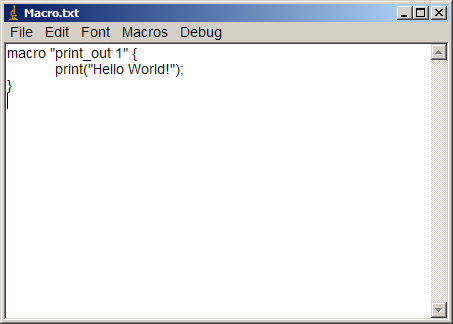
\includegraphics[scale=0.6]{fig/editor_helloworld_IJ.png}
\caption{Macro Editor of ImageJ} \label{fig_MacroEditor}
\end{center}
\end{figure}

\begin{figure}[hbtp]
\begin{center}
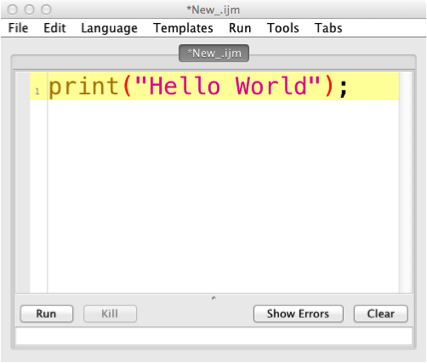
\includegraphics[scale=1.0]{fig/editor_helloworld_singleline.png}
\caption{Script Editor of the Fiji distribution} \label{fig_ScriptEditor}
\end{center}
\end{figure}

From the macro editor menu, running the code by \ijmenu{[Macros->
Run Macro]}\footnote{"Macros" in the menu appears only when the macro editing
window is active}. You could also run the code by shortcut keys (Windows:
ctrl-r, OSX command-r) as well. 
 
\begin{indentFiji}
Fiji:  Use \ijmenu{[Run -> Run]} from the script editor menu. Shortcut keys are
same as in ImageJ. You could also use ``run'' button in the script editor. 
\end{indentFiji}
This will create a new window "Log". Within the log window, "Hello World" will
be printed.

\begin{figure}[hbtp]
\begin{center}
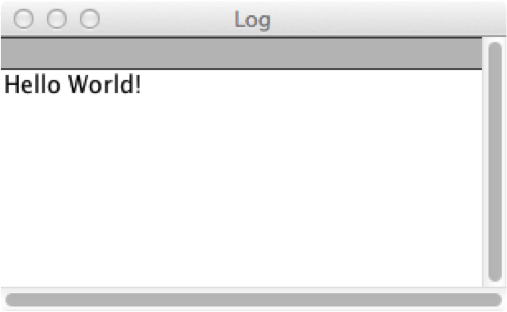
\includegraphics[scale=1.0]{fig/helloworld_logwindow.png}
\caption{Hello World Output} \label{fig_HelloWorldLog}
\end{center}
\end{figure}

Explanation for the Code 1:\\
\begin{itemize}
\item line 1: You are declaring that a macro code starts and the code is contained between 
curly braces \{\}. "print\_out" will be the name of macro. 

\item line2: print() function orders ImageJ to print out the content within the parenthesis 
in the "Log" window. The text to be printed must be contained within the double quotes (""). 
The best reference for ImageJ macro functions is in the ImageJ web site
\footnote{\url{http://rsbweb.nih.gov/ij/developer/macro/functions.html}}. 
For example, you could find definition of print("") function on the web site as quoted below:\\
%\item
\begin{indentCom}
%\begin{minipage}[c][18em][c]{0.85\textwidth}
\fbox{
\parbox[b][20em][c]{0.80\textwidth}{
\textbf{print(string)}\\
Outputs a string to the "Log" window. Numeric arguments are automatically converted to strings. 
The print() function accepts multiple arguments. For example, you can use print(x,y,width, height) 
instead of print(x+" "+y+" "+width+" "+height). 
If the first argument is a file handle returned by File.open(path), 
then the second is saved in the referred file (see SaveTextFileDemo).

Numeric expressions are automatically converted to strings using four decimal places, 
or use the \ilcom{d2s} function to specify the decimal places. 
For example, print(2/3) outputs "0.6667" but print(d2s(2/3,1)) outputs "0.7".
}
}
\end{indentCom}

\item line 3: a brace tells ImageJ that the code "print\_out" finishes at this line.  
\end{itemize}
So that was the very basic of how you use a macro. To integrate the macro into the ImageJ Menu bar, 
the macro must be "installed". To do so, in the editor menu, \ijmenu{[Macros -> Install Macros]} 
\begin{indentFiji}
Fiji: [Run -> Install Macro]).
\end{indentFiji}
Check IJ menu \ijmenu{[Macros -> ]} to see that the macro is now in the menu.\\


\begin{figure}[htbp]
\begin{center}
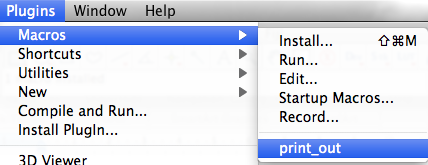
\includegraphics[scale=0.6]{fig/firstMacroInMenu.png}
\caption{Macro Now in ImageJ menu} \label{fig_MacroInMenu}
\end{center}
\end{figure}

Macro can be saved as a file and can be directly installed also. 
In the editor, do \ijmenu{[File -> Save]}. Saving dialogue window appears, 
and just save the file wherever you can remember afterwards . 
To install the macro, do \ijmenu{[PlugIns -> Macro -> Install\ldots]} 
Select the macro file you want to install.\\

%\begin{indentexercise}{1cm}
\begin{indentexercise}{1}
\item Add another line \texttt{"print("\textbackslash{}\textbackslash{}Clear");"} 
after the second line (below, code 1.5. don't forget the semi-colon at the end!). 
\item \lstinputlisting{code/code01_5.ijm}
Then test also another macro when you insert the same function in the third line (code 1.75). 
What happened?  
\item \lstinputlisting{code/code01_75.ijm}
\end{indentexercise}

\begin{indentexercise}{2}
\item Try modifying the third line in code 1.5 
and check that the modified text will be printed in the "Log" window. \\
\end{indentexercise}

\begin{indentexercise}{3}
\item Multiple macros can exist in a single file. We call this \textbf{"macro sets"}. 
Duplicate the code you wrote by copying and pasting it under the first macro. 
The second macro should have a different name. In the example shown in fig.
\ref{fig_MacroSetInMenu}, the second macro is named "pirnt\_out2".
\end{indentexercise}

\begin{figure}[h!]
\begin{center}
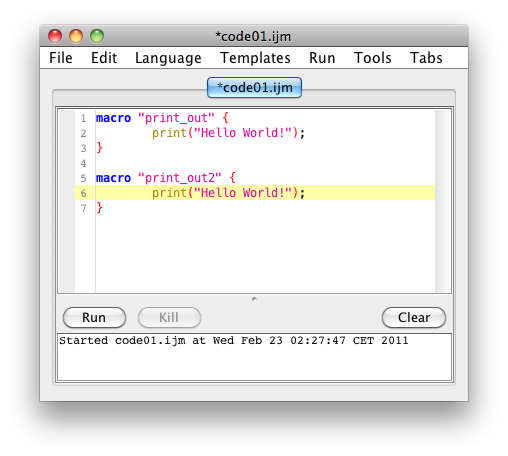
\includegraphics[scale=0.6]{fig/editor_MacroSet.png}
\caption{Macro Set} \label{fig_MacroSetInMenu}
\end{center}
\end{figure}
When macro is properly declared in this way, you could install the macro to have it as a menu item. To do so, in the editor menu select: 
\begin{indentFiji}
[Run -> Install Macro]).
\end{indentFiji}
In the main menu you should no be able to see the macro names under \ijmenu{[Plugins > Macros > ]}.


\subsection{Variables and Strings}
Texts such as "Hello World!" can be represented by a variable 
\footnote{there is no declaration of types, such as number or string, in ImageJ macro.}.
Let's understand this by examining a short macro below.
\lstinputlisting{code/code02.ijm}

\ilcom{text} is a "String Variable" or simply a "String". 
ImageJ prepares a memory space for this variable, and you can change the content by re-defining the content. Two (or maybe more) variables could be used to construct another variable. 

\lstinputlisting{code/code03.ijm}

The above operation concatenates content of \ilcom{text2} to the content of \ilcom{text1} and produces a third variable \ilcom{text3} that holds the result of concatenation. It should be noted here, that macro has two ways of usage for \ilcom{+}. What we tested in above is ``concatenation''. Another usage is ``addition'' in the next section. 

\begin{indentexercise}{1}
\item Add more string variables and make a longer sentence.\\
\end{indentexercise}


It is also possible to store a number in a variable. For example, \\
\begin{lstlisting}[numbers=none]
text = 256;
\end{lstlisting}
With this assignment, the variable is now a "numerical variable" or simply "variable". 
In other programming languages such as C or Java, difference between numbers and characters matters a lot. 
In ImageJ macro you do not have to care whether the variable is number or string (we call them ``types'') ad they are defined automatically by the type of value provided for a variable, and this makes the macro coding to be light and easy. However, since types are implicitly defined without declaration it could cause simple mistakes such as type mismatching. 
So be sure keep the difference in types DOES matter but they are not shown in the code. We will see an example of such confusion, 
and also a way to avoid the confusion. 

Test the following macro to see how the numerical variable works. 
\lstinputlisting{code/code04.ijm}
Did you get some results printed out? It should, but you should read the code carefully as there is a small trick in this code.  This trick is something special in IJ macro language compared to other general scripting languages. 

You might have noticed a strange expression at line 8, in the way it assigns the variable \ilcom{txt}. 
It starts with double quotation marks. \\
%\lstinputlisting[language=Java, linerange={8-8}, numbers=none]{code/code04.ijm}
\begin{lstlisting}[numbers=none]
txt= "" + a + "+" + b + "=" + c;
\end{lstlisting}
Seemingly this looks like meaningless. 
If you define ilcom{txt} without the first "useless" quotation marks, then it will be like\\
\begin{lstlisting}[numbers=none]
txt= a + "+"+ b + "=" + c;
\end{lstlisting}
Theoretically this should work, 
since the double quote does not have any content so its presence should be meaningless. But if you try to run this what it seems to be straight-forward assignment, 
ImageJ returns an error message. 

\begin{figure}[htbp]
\begin{center}
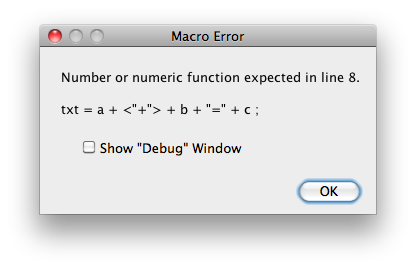
\includegraphics[scale=0.6]{fig/ErrorStringNumericFunction.png}
\caption{Error with Variable Assignment} \label{fig_ErrorVariable}
\end{center}
\end{figure}

This is because when ImageJ scans through the macro from top to bottom, line by line, 
it reaches the line for the assignment of the variable \ilcom{txt} and first sees the variable \ilcom{a} and interprets that \ilcom{txt} should be a numerical variable 
(or function), since \ilcom{a} is known to be a number as it was defined so in one of the lines above. Then ImageJ goes on interpreting rightward thinking that this is math. Then finding a "+" which surprisingly is a character
ImageJ cannot interpret string variable within a numerical function, so it returns an error message. The macro aborts.  

To overcome this problem, the programmer can tell ImageJ that 
\textit{txt} is a string function at the beginning of the assignment 
by putting a set of double quote. This tells the interpreter that this assignment is a string concatenation assignment and not a numerical assignment. 
ImageJ does handle numerical values within string function, 
so the line is interpreted without problem and prints out the result successfully. Note that such confusion of string and numerical types are rarely seen in general scripting languages and specific to ImageJ macro language.

\begin{indentexercise}{2}
Modify the code 4, so that the calculation involves subtraction (-), multiplication (*) and division (/). 
\end{indentexercise}

\subsection{Parameter Input by User}
At some point you might want to make a macro to ask the user to input numerical
values or file names. We now learn how to do that, by first examining the
following code. Run the code first.
\lstinputlisting{code/code05.ijm}
Running this macro,  a dialogue window pops-up.

\begin{figure}[htbp]
\begin{center}
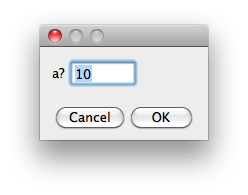
\includegraphics[scale=0.6]{fig/getNumberDialog.png}
\caption{getNumber Dialog} \label{fig_getNUmber}
\end{center}
\end{figure}

The function \textit{getNumber} consists of two parameters (programmers call such parameters "arguments" so we use this word in the reminder of this textbook).
\begin{indentCom}
\textbf{getNumber}(message string, default number)
\end{indentCom}
The first argument is a string wrapped by double quotes (see code 5, line 3
and 4). This string will appear in the dialog window such as shown above. 
Default number will appear in the input field in the dialog window, 
and the user is expected to modifies this default number. 
When OK button is clicked, the number given by the user will be returned to
the macro and then substituted to a variable. In the above case, this could be
either \textit{a} or \textit{b}.
 
To ask a user for providing a string in dialog, following is an example. 
\lstinputlisting[morekeywords={*, getString}]{code/code06.ijm}

The function \textbf{getString} also has two arguments, 
and only the difference is that the user input will be treated as a string. \\

\begin{indentexercise}{1}
Run the code 6 and input 1 for a and 2 for b. What happened? Explain the reason. 
\end{indentexercise}

\subsection{Recording ImageJ macro functions}
There are many commands in ImageJ as you could see them by exploring the menu tree. In ImageJ native distribbution, there are ca. 500 commands. In the Fiji distribution, there are 900+ commands. Some plugins are not macro-ready, but except for those spacial cases almost all of these commands can be accessed by build-in macro functions. We then encounter a problem: how do we find a macro function that does what we want to do?

To show you how to find a function, we write a small macro that creates a new image, adds noise, blurs this image by Gaussian blurring, and then thresholds the image. There is a convenient tool called \textbf{Command Recorder}. 
Do \ijmenu{[PlugIns -> Macros -> Record\ldots]}. A window shown in figure
\ref{fig_macroRecorderBlank} opens.

\begin{figure}[htbp]
\begin{center}
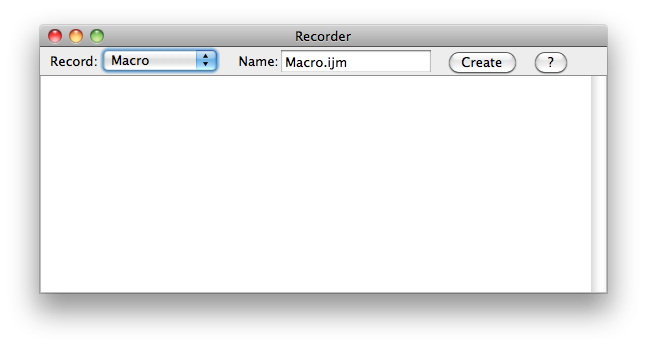
\includegraphics[scale=0.6]{fig/MacroRecorderBlank.png}
\caption{Macro Recorder} \label{fig_macroRecorderBlank}
\end{center}
\end{figure}

All the menu commands that you execute will be printed out as a history of macro functions in this window. For composing a macro using this recorder, we first do the processing manually from the menu as follows. 
\begin{itemize}
  \item Prepare a new image using \ijmenu{[File -> New]} command. The size of the image can be anything.
  \item Then do \ijmenu{[Process -> Noise -> Salt and Pepper]} (Fig.
  \ref{fig_SaltAndPepper}).
  \item \ijmenu{[Process -> Filters -> Gaussian Blur]} (use Sigma = 2.0).
  \item \ijmenu{[Image -> Adjust -> Threshold\ldots]}. Toggle the slider to make
  signals red. Check "Dark Background", then click "Apply".
\end{itemize}
 
\begin{figure}[htbp]
\begin{center}
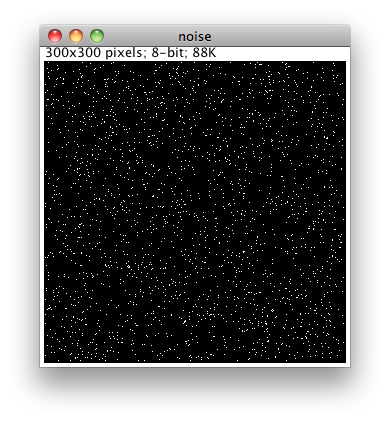
\includegraphics[scale=0.6]{fig/SaltandPepper300.png}
\caption{A demo image for Recording Macro} 
\label{fig_SaltAndPepper}
\end{center}
\end{figure}

Now, check the Command Recorder window. 
It should now look like Fig. \ref{fig_macroRecorderFilled}. 
Each line is a macro function that corresponds to a menu command you selected.

\begin{figure}[htbp]
\begin{center}
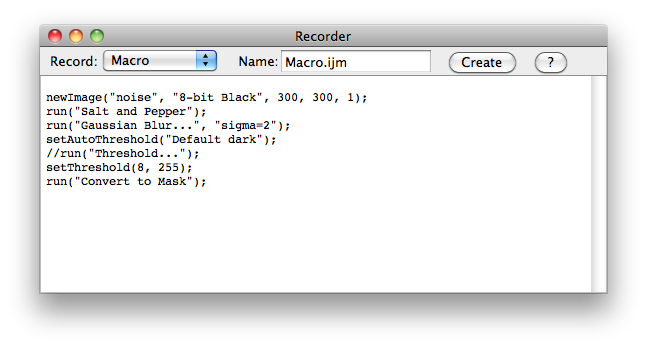
\includegraphics[scale=0.6]{fig/MacroRecorderFilled.png}
\caption{Macro Recorder after some lines Recorded} 
\label{fig_macroRecorderFilled}
\end{center}
\end{figure}

These texts generated in the recorder can be used as it is in your macro.  You could copy and paste them\footnote{In case of OSX, you might probably need to click ``Create'' button to generate a duplicate of macro functions in a new script window. Then you could copy the macro functions from there.}. Compose a macro like below by copying and pasting the macro functions in the recorder.  Delete the lines that are commented out (lines that begin with "//" are lines that are skipped by the macro interpreter).
\lstinputlisting{code/code06_9.ijm}

Run the macro! \ldots I hope that you are amazed by now with the power of Macro
Recorder! Now, you could simply add a line at the top and bottom to package this in a named macro by curly braces. This is optional in the current case, but it's always good to keep your macro packaged since the boundary of the macro becomes clear. 
 
\lstinputlisting{code/code07.ijm}

The third line in the above macro has a function \ilcom{newImage()}. This
function creates a new image. It has five arguments (in coding jargon, we say
there are "five arguments"). To know what these arguments are, 
the quickest way is to read the Build-In Macro Function page in ImageJ web site\footnote{\url{http://rsbweb.nih.gov/ij/developer/macro/functions.html}}.  
In case of the function \ilcom{newImage}, the description looks like this. 

\begin{indentCom}

\fbox{
\parbox[b][16em][c]{0.80\textwidth}{
\textbf{newImage}(title, type, width, height, depth)\\
Opens a new image or stack using the name title. 
The string type should contain "8-bit", "16-bit", "32-bit" or "RGB". 
In addition, it can contain "white", "black" or "ramp" (the default is "white"). 
As an example, use "16-bit ramp" to create a 16-bit image containing a grayscale ramp.  Width and height specify the width and height of the image in pixels.  Depth specifies the number of stack slices.
}}
\end{indentCom}
Using this information, you can modify the macro to change the size of the image.

\begin{indentexercise}{1}
Modify the code 8, so that user can input the desired Gaussian sigma.
\end{indentexercise}

Other optional lines you could add to the macro are ``comments''. This does not affect the macro but adding some comment about what the macro does helps you to understand what the macro is doing when you open the file some time later. There are two ways to add comment. One is the \textbf{block comment}. Texts bounded by \ilcom{ /*} and \ilcom{*/} will be ignored by interpreter. Another is the line comment. Texts in a line starting with double slash \ilcom{//} will be ignored by the interpreter. Below is an example of commenting code 07. 

\lstinputlisting{code/code07_1.ijm}


\subsection{Batch Processing using "batch macro" function}
In above macro, list of functions were wrapped inside macro "title"\{ code \} 
so that these macro functions could be executed by single command from menu. 
To apply such a sequence of macro functions for many images in a single folder 
(say you have one-thousand images you want to contrast enhance and also to Gaussian-blur), 
there are two ways. One way is to further extend the macro by adding file-accessing macro functions and 
looping those functions (you will learn this later). 
Another way is to do such "batch processing" by copy and pasting list of
macro functions to batch-processing interface. 
This interface could be used by \ijmenu{[Process -> Batch -> Macro]}

\begin{figure}[htbp]
\begin{center}
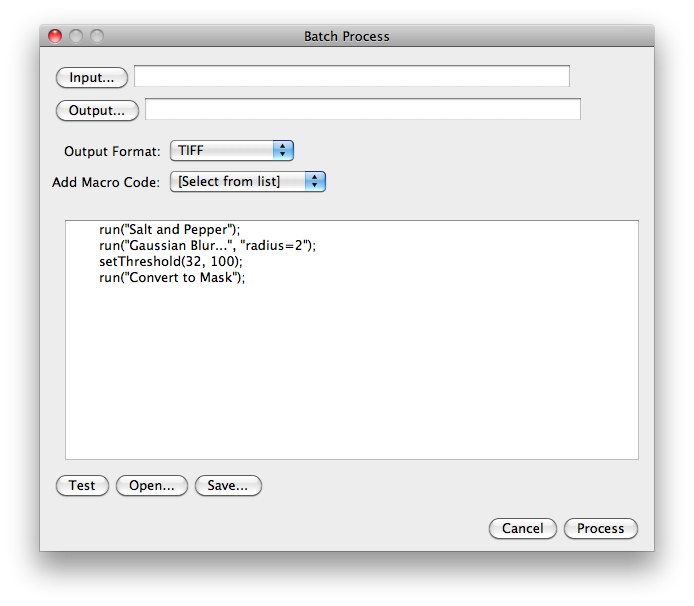
\includegraphics[scale=0.4]{fig/BatchProcessing.png}
\caption{Batch Processing Dialog} \label{fig_BatchProcessInterface}
\end{center}
\end{figure}

In "Input" field, select the folder where image files are stored. 
In output field, select a destination folder where processed images will be stored. 
You then copy and paste the list of macro functions in the code field such as 
shown in Fig. \ref{fig_BatchProcessInterface}. 
In the case shown in this figure, line 6 to 9 was copied and pasted. 
Clicking "Process" button will start the processing.
\newpage

\section{Conditions and Loops}
In many cases, we want to iterate certain processing steps many times (see "Loops" in the figure \ref{fig_scriptscheme}), or we want to limit some of the process in the program only for certain situations (see "Conditions": in the figure \ref{fig_scriptscheme}). In this section we learn how to include these loops and conditional behaviors into macro. 

\begin{figure}[htbp]
\begin{center}
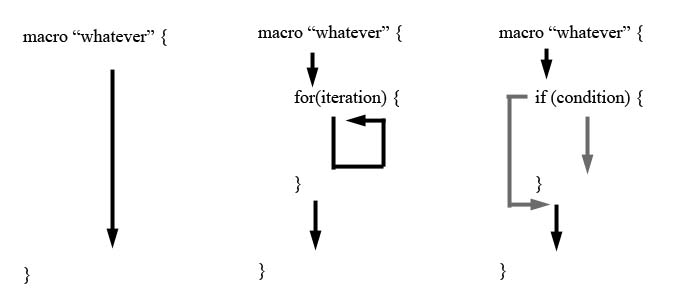
\includegraphics[width=\textwidth]{fig/fig23_1_ScriptSchemes.png}
\caption{Schematic view of conditions and loops. Straightly top to bottom, line by line processing (left) and macro with loops (middle) and with a condition (right).} \label{fig_scriptscheme}
\end{center}
\end{figure}

\subsection{Loop: for-looping}
Here is a simple example macro using for-loop. Write the macro in your editor and run it. 
\lstinputlisting[morekeywords={*, for}]{code/code09.ijm}
The result should look like figure \ref{fig_whateverOut}.

%whatever x 5 figure
\begin{figure}[h!]
\begin{center}
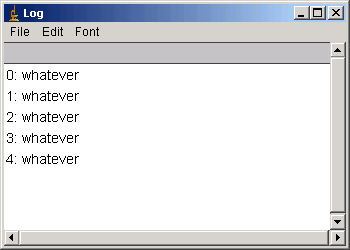
\includegraphics[scale=0.6]{fig/fig2311_whatever5.png}
\caption{Code 9 output in Log Window}
\label{fig_whateverOut}
\end{center}
\end{figure}

\begin{itemize}
\item Line 3 asks the user to input a string (we did this already). 
If user does not change the default text ("whatever") and click "OK", 
then the macro interpreter proceeds to line 4.

\item Line 4 \ilcom{for( i = 0 ; i < 5 ; i+= 1)} sets the number of loops. 
Three parameters are required for "for" loop. The first parameter defines the variable used for the counting loop and its initial value (\ilcom{i = 0}). The second parameter sets the condition for exiting from the loop (\ilcom{i < 5}). Third parameter sets the step size of i, meaning that how much value is added per loop (\ilcom{i += 1}, could also be subtraction, multiplication, division e.g. \ilcom{i -= 1}).
Spaces between variables, numbers, operators and separators (e.g. semicolon, parenthesis) can be ignored and they could be written continuously. Macro runs without those spaces. However, this is not recommended for keeping a better readability of the code. Don't try to rush, make spaces!
\item After this \ilcom{for(\ldots;\ldots;\ldots)} statement, there is a brace (\{) at the end of line 4 and the second one  (\}) in the line 6. These curly braces tell ImageJ to loop macro functions in between so the function in line 5 will be iterated according to the parameters defined in the parenthesis of \ilcom{for}. 
Between braces, you could add as many more lines of macro functions as you want, including inner \ilcom{for}-loops and \ilcom{if-else} conditions.
\end{itemize}
So when the macro interpreter reaches line 4 and sees \ilcom{for(}, it starts looking inside the parenthesis and defines that the counting starts with 0 using a variable \ilcom{i}, and then line 5 is executed. The macro prints out "0 \ensuremath\colon whatever" using the content of \ilcom{i}, string \ilcom{\ensuremath\colon} and the string variable \ilcom{txt}. 
Then in line 6 interpreter sees the boundary \ilcom{\}} and goes back to line 4 and adds 1 to i (because of \ilcom{i+=1}). i = 1 then, so \ilcom{i<5} is true. The interpreter proceeds to line 5 and executes the macro function and prints out "1\ensuremath\colon whatever".  Such looping will continue until i = 5, since only by then \ilcom{i<5} is no longer true so interpreter exits from the for-loop. \\


\begin{indentexercise}{1}
(1) Change the first parameter in \ilcom{for(i=0;i<5;i+=1)} so that the macro prints out only 1 line. 

(2) Change the second parameter in \ilcom{for(i=0;i<5;i+=1)} so that the macro prints out 10 lines. 

(3) Change the third parameter in \ilcom{for(i=0;i<5;i+=1)} so that the macro prints out 10 lines. 
\end{indentexercise}


\subsubsection{Stack Analysis by for-looping}
\label{sec:forloopStack}
One of frequently encountered tasks is image stack management, 
such as measuring dynamics or multi-frame processing. 
Many ImageJ functions work with only single frame within a stack. 
Without macro programming, you need to execute the command while you flip the frame manually. 
Macro programming enables you to automate this process. 
Here is an example of measuring intensity change over time\footnote{What we write as macro here could be done with a single command \ilcom{[Image > Stacks > Plot Z-Profile]} but this only measures intensity. If you want to measure other values such as the minimum intensity, a macro should be written. }. 
\lstinputlisting[morekeywords={*, run, setSlice, nSlices}]{code/code10.ijm}
\begin{itemize}
\item Line 3: \ilcom{nSlices} is a macro function that returns the number of slices in the active stack. 

\item Line 4: Sets measurement parameters, from the menu would be \ilcom{[Analyze > Set measurements\ldots]}. In this case "mean min integrated" is added as part of the second argument. ``mean'' is the mean intensity, ``min'' is the minimum intensity and ``integrated'' is integrated density (total intensity). These keys for measured parameters could be known by using the command recorder. 
You do not have to care for now about the "redirect" argument. ``decimal'' is the number of digits to 
the right of the decimal point in real numbers displayed in the results table. 

\item Line 5: clears the results table. 

\item Line 6 to 9 is the loop. Loop starts from count i=0, and ends at i=frame-1. \ilcom{i++} is another way of writing \ilcom{i = i + 1}, so the increment is 1.  

\item Line 7: calculates the current frame number. 

\item Line 8: \ilcom{setSlice} function sets the frame according to the frame number calculated in line 6. 

\item Line 9:  actual measurement is done. 
Result will be recorded in the memory and will be displayed in the Results table window. 
\end{itemize}

Open an example stack \textbf{1703-2(3s-20s).stk}
\footnote{Some of you may realize that you used this sequence 
in the Image Processing / Analysis Course for learning 
stack measurements using Z-profiler \ilcom{[Image > Stacks > Plot Z-Profile]}. Now, you can program similar 
device in macro. 
Good thing about the custom program
is that you will be able to modify the program further to add more functions.
For example, You could measure the time course of standard deviation of
intensity within the selected ROI.}. This is a short sequence of FRAP analysis,
so the edge of the one of the cells is bleached and then fluorescence signal at that bleached position recovers by time. 
Select the frapped region by ROI tool (such as in the figure below). 
Execute the macro. Results will be printed in the Results window (see the table in the figure right: this table is showing only "Mean" column as only ``Mean Intensity'' was selected in the measurement option). 

\begin{figure}[htbp]
 \centering
% \subfloat[Setting a Segmented ROI at the FRAPped area.]{\label{fig:gull}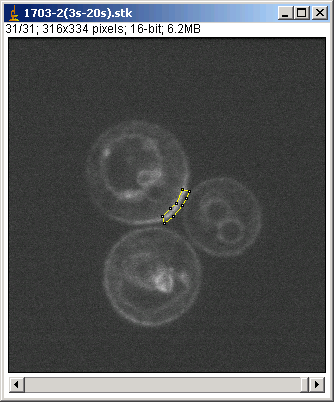
\includegraphics[width=0.3\textwidth]{fig/fig2321a_frapimage.png}}
 \subfloat[]{\label{fig:frapimage}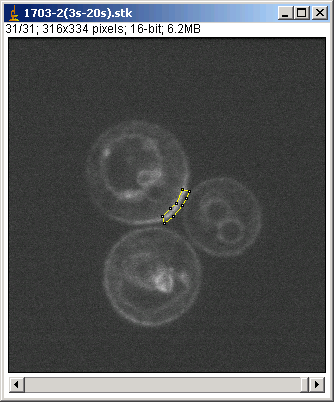
\includegraphics[height = 60mm]{fig/fig2321a_frapimage.png}}
 \quad
 \subfloat[]{\label{fig:frapmeasured}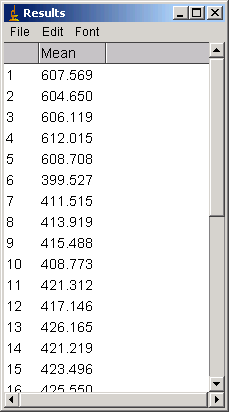
\includegraphics[height = 60mm]{fig/fig2321b_frapResults.png}}
 \caption{Measuring Stack Intensity Series. (a) Setting a Segmented ROI at the FRAPped area. (b) Results of Measuring Mean Intensity Dynamics.}
 \label{fig:frapresults}
\end{figure}


Measurement parameters can be added as argument by modifying the line 4 in the code 10. "Set Measurement" could be added with more parameters to be measured, and the digits after the decimal point could be increased by increasing the number after ``decimal=''. For example, 
\begin{lstlisting}[numbers=none]
run("Set Measurements...", "area mean standard modal min centroid center perimeter bounding integrated median stack redirect=None decimal=5");
\end{lstlisting}

\begin{indentexercise}{1}
Modify code 10 to include more measurement parameters (whatever you like), and test the macro. Check the results. 
\end{indentexercise}

% figure
\begin{figure}[htbp]
\begin{center}
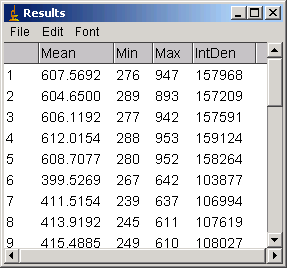
\includegraphics[scale=0.5]{fig/fig2322_moreResultsTable.png}
\caption{An example result after adding more measurement parameters.}
\label{fig_MoreMeasurementPara}
\end{center}
\end{figure} 


\subsection{Loop: while-looping}

Another way of letting a part of macro to loop is \textbf{while}-statement. In this case, iteration is not defined strictly. Looping continues until certain condition is met. As soon as the condition is violated, macro interpreter goes out from the loop.

\subsubsection{Basics of while statement}
Here is a simple example macro using \ilcom{while}.
\lstinputlisting[morekeywords={*, while}]{code/code11.ijm}
This macro prints out characters 0 to 90 with a 10 increment. 

%figure
\begin{figure}[htbp]
\begin{center}
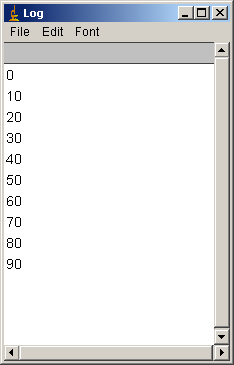
\includegraphics[scale=0.4]{fig/fig2331_Code11out.png}
\caption{Output of code 11}
\label{fig:code11 output}
\end{center}
\end{figure} 

\begin{itemize}
\item line 3: The macro interpreter first assigns 0 to the counter.
\item line 4: The interpreter evaluates if the counter value is less than or equal to 90. Since counter is initially 0\ldots 
\item line 5: Printing function is executed. 
\item line 6: counter is added with 10. 
\item line 7: the interpreter realizes the end of "while" boundary and goes back to line 4. Since counter= 10 <= 90, line 5 is again executed\ldots and so on. When counter becomes 100 in line 6 after several more loops, counter is no longer <=90. So the interpreter goes out from the loop, moves to line 8. Then the macro is terminated.
\end{itemize}

Line 5 could be written in the following way as well.
\begin{lstlisting}[numbers=none]
counter += 10;
\end{lstlisting}
This means that "counter" is added with 10. Similarly, subtracting 10 from counter is 
\begin{lstlisting}[numbers=none]
counter -= 10;
\end{lstlisting}
Multiplication is 
\begin{lstlisting}[numbers=none]
counter *= 10;
\end{lstlisting}
Division is
\begin{lstlisting}[numbers=none]
counter /= 10;
\end{lstlisting}
If the increment is 1 or -1, (counter +=1 or counter-=1), then one could also write them  as 
\begin{lstlisting}[numbers=none]
counter++;
 or 
counter--;
\end{lstlisting}
These two last macro functions are said to work faster than +=1 or -=1, but I myself do not see much difference. Computers are fast enough these days. 

\begin{indentexercise}{1}
(1) Try changing code 11 so that it uses "+=" sign.\\
(2) Change code 11 so that it uses "++" sign, and prints out integers from 0 to 9.\\
\end{indentexercise}
Evaluation of \ilcom{while} condition could also be at the end of loop. In this case, \ilcom{do} should be stated at the beginning of the loop. With do-while combination, the loop is always executed at least once, regardless of the condition defined by \ilcom{while} since macro interpreter reads lines from top to bottom. Try with the following exercise.

\begin{indentexercise}{2}
Change line 4 of code 11 to \ilcom{while (counter <0)} and check the effect (see below).
\end{indentexercise}

\lstinputlisting[morekeywords={*, while}]{code/code11_5.ijm}

Condition for the while-statement could be various. Here is a small list of comparison operators.

\begin{indentCom}
 \begin{tabular*}{0.5\textwidth}{ l r }
< & less than \\
<= & less than or equal\\ 
> & greater than\\ 
>= & greater than or equal to\\
== & equal\\
!= & not equal\\
 \end{tabular*}
\end{indentCom}

\begin{indentexercise}{3}
Modify code 11 so that the macro prints out numbers from 200 to 100, with an increment of -10. 
\end{indentexercise}

\subsubsection{Why is there while-loop?}

An often raised question with the while-loop is why do we have two types of loops, 
the for-loop and the while-loop. Answering to this question, they have different
flexibility. The for-loop is rather solid and the while-loop is more flexible. In the
example code below, the user is asked for a correct number and if the answer is wrong, the
question is asked 5 times repeatedly. Number of loop is not determined by the
programmer, but interactively when the code is running. We will study
the branching of the program based on if-else in the next section.  

\lstinputlisting[morekeywords={*, while}]{code/code11_6.ijm}

Writing a similar code using the for-loop is possible but the code becomes tricky.
Below is the for-loop version of the above code.  

\lstinputlisting[morekeywords={*, for}]{code/code11_7.ijm}

Note that the third argument of for-loop is missing. Since the variable
\ilcom{correct} does not change as long as the answer is wrong, we leave it not
incrementing nor decrementing. In such case we can leave the third argument
vacant. 

\subsection{Conditions: if-else statements}
\subsubsection{Introducing if-else}
A macro program could have parts which are executed depending on some
conditions.
Here is an example of macro with conditions.
\lstinputlisting[morekeywords={*, if}]{code/code12.ijm}
\begin{itemize}
\item Line 3 The macro asks user to input a number and the number is substituted to the variable input\_num.
\item Line 4 Content of input\_num is evaluated. If input\_num is equal to 5, line 5 is executed and prints out the message in the Log window. Otherwise macro interpreter jumps to line 7, and ends the operation.  By adding "else" which will be executed if input\_num is not 5, the macro prints out message in all cases (see code 12.5 for this if - else case). 
\item Line 4 We used double equal signs for evaluating the value in the right side and the left side (e.g. \ilcom{if (a==5)}). 
Note that the role of the sign \ilcom{=} is different from assignments, or substitution (e.g. \ilcom{a = b + c}).
\end{itemize}
%figure
\begin{figure}[htbp]
\begin{center}
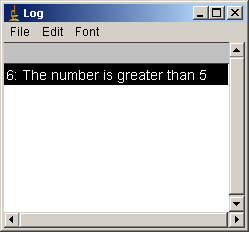
\includegraphics[scale=0.6]{fig/fig2341_code12out.png}
\caption{Output of code 12}
\label{fig:code12 output}
\end{center}
\end{figure} 

Now, we examine the content between 
parenthesis after ``if'' in more detail. 
Write the following code in your script editor and run it.
\lstinputlisting[morekeywords={*, ==}]{code/code12_1.ijm}
The output in the log window should be \textit{1} indicating that ``\ilcom{(5 ==
5)}'' is \textit{1}. Next, modify the code like below and run it.
\lstinputlisting[morekeywords={*, ==}]{code/code12_2.ijm}
The output is now 0, indicating that ``\ilcom{(5 == 4)}'' is
0.
What double equal signs \ilcom{==} are doing in these
examples are comparison of numbers in the left and the right side, and if
the numbers are the same, it returns 1 and if they are not the same, it returns 0. 1 and
0 actually are representing \textbf{true} (= 1) or \textbf{false} (= 0), the
\textbf{boolean values}.

We could also test if they are NOT equal. For this, replace \ilcom{==} by
\ilcom{!=}.
\lstinputlisting[morekeywords={*, !=}]{code/code12_3.ijm}
Run the code above, and it returns 1, because 5 is NOT 4 and that is true. Now,
you could introduce the \textit{if} again as follows.
\lstinputlisting[morekeywords={*, if, else}]{code/code12_35.ijm}
In the parenthesis after ``if'', there is obvious TRUE statement (5 is not 4).
This is true, so the macro function bounded by curly braces is executed, which is to
print out ``true'' in the log window.

Try changing the line 2 to \ilcom{if (5 == 4)}. Running this prints nothing
in the log window, because 5 is not 4 (FALSE!) so that the macro function in
line 3 is ignored. To avoid such ignorant no-output behavior, you could add
``else'' as follows.

\lstinputlisting[morekeywords={*, if, else}]{code/code12_4.ijm}

The code works also with the direct true or false
declaration inside the if parenthesis. Try the following code.

\lstinputlisting[morekeywords={*, if, else}]{code/code12_5.ijm}

The above prints two lines of ``false!'' in the log window. You could replace
the if parenthesis values to 1 and true to check that it works as well. 

By now, it is probably pretty clear to you wi what is going on in the code below. 
\lstinputlisting[morekeywords={*, if, else}]{code/code12_6.ijm}

\subsubsection{Complex Conditions}
In many cases, you might need to evaluate the condition of multiple variables at once. 
For such demands, several different comparisons can be combined by using following Boolean operators. 

\begin{indentCom}
 \begin{tabular*}{0.5\textwidth}{ l l }
\&\& & boolean AND\\
|| & boolean OR\\
\end{tabular*}
\end{indentCom}

Let's first test what these symbols do by directly using
\ilcom{true} and \ilcom{false} in macro.
\lstinputlisting[morekeywords={*, if, else}]{code/code12_65.ijm}
When you run this code as it is, line 4 and line 8 are both executed and prints
the messages. For the first \ilcom{if} parenthesis, \ilcom{\&\&} operator tests if
both sides are true. If both are indeed true, it returns true (1), and that is
the case above. If one of them or both are false, then \ilcom{\&\&}
operator returns false(0). 

On the other hand, in the second if parenthesis,
\ilcom{||} operator tests if one of the two sides is true. Since both are
true in the above code, OR operator returns true because at least one of them is
true. Only when both sides are false, the returned value becomes false (0).

\begin{indentexercise}{1}
Change the values of \ilcom{a} and \ilcom{b} in code 12\_65 to \ilcom{false} and
compose other three possible combinations (e.g. \ilcom{a = true}, \ilcom{b = false} will print
only one line).
Check the output. Change the values of \ilcom{a} and \ilcom{b} also to 0 and/or
1 and check the results. 
\end{indentexercise}

Here is a more realistic example (though not very useful), an extended version
of code 16\_6.
\lstinputlisting[morekeywords={*, if, else}]{code/code12_75.ijm}
\begin{itemize}
\item Line 4 and 5 ask user to input two parameters.
\item Line 6 is for setting a string variable, to abbreviate a long string assignment that appears four times in the macro.
\item Line 7 evaluates these input parameters by comparing each of them separately, but the decision is made by associating two decisions with \ilcom{\&\&}. 
%\item Text after "//" is called comment. Text after this double slash will not be evaluated by the macro interpreter. Comments helps programmers later for remembering (or letting other programmer to understand) the purpose of the line. 
\item Line 10, != compares left and right sides of the operators and returns true if they are NOT equal.   
\end{itemize}
From line 10 to 17, there are several layers of conditions. Macro programmer should use tab-shifting for deeper condition layers as above for the visibility of code. Easy-to-understand code helps the programmer oneself to debug afterward, and also for other programmers who might reuse the code.
\subsubsection{Application of if-statement}
\label{sec:dotmove}

As an application of looping and conditions, we write a macro that produces an animation of moving dot. User inputs the speed of the dot, and then the animation is generated. 
In the animation (which actually is a stack) the dot moves horizontally and bounces back from the edge
of the frame. 
\ilcom(if) operator is used to switch the movement direction.
\lstinputlisting[morekeywords={*, setForegroundColor, setBackgroundColor, if}]{code/code13.ijm}

\begin{itemize}
\item Lines 4 to 11: Set parameters for drawing a dot. It is also possible to directly use numerical values in the later lines, but for the sake of readability of the code, and also for possible later extension of the code, it is always better to use easy-to-understand variable names and explicitly define them before the main part starts. 
\end{itemize}
A short note on the x-y coordinate system in digital images: Since digital image is a matrix of numbers, each pixel position is represented as coordinates. The top left corner of image is the position (x, y) = (0, 0). X increases horizontally towards right side of the image. Y increases vertically towards the bottom of the image.  In line 9, y-position of the dot is defined to be placed in the middle of the vertical axis. 
\begin{itemize}
\item Lines 14, 15: These lines set the drawing and background color. Three arguments are for  intensity of each RGB component. Here the image is in grayscale so all the RGB components are set to the same value. 0 is black, and \ilcom{int} is white (255).
\item Line 14 asks the user to input the speed of the dot movement.
\item Lines 16, 17 prepares a new stack with parameters defined in lines 7, 8 and 9.
\item Lines 21 to 34 is the loop for drawing moving dot. Loop will be iterated from the starting frame until the last frame. Line 21 creates an oval Region-of-Interest (ROI), which will be filled in line 22 with the foreground color that was already set in the line 14. \ilcom{makeOval} function is explained in the Built-on function page as follows.

\begin{indentCom}
\textbf{makeOval}(x, y, width, height)\\
Creates an elliptical selection, where (x,y) defines the upper left corner of the bounding rectangle of the ellipse. 
\end{indentCom}
\item Line 27: Shifts the x position of the dot by ``speed'' distance. 
\item Line 28: if the position calculated in the line 27 exceeds the boundary, either left \ilcom{(x\_position < 0)} OR right \ilcom{(x\_position > (w-sizenum))}, then the direction of movement is switched by multiplying -1.
\end{itemize}
\begin{indentexercise}{2}
Modify code 13 that the dot moves up and down vertically. Change the stack width and height as well. 

If you are successful with this, try further on to extend the code so that the dot moves both in x and y directions. For this, you need to have two independent speed \ilcom{xspeed} and \ilcom{yspeed} since change in the direction by bouncing should be independent in x and y. 
\end{indentexercise}

\subsubsection{Application of "while" and "if" in image processing.}
Now, we try solving a problem with image thresholding by an application of 
\ilcom{while} loop in a macro. Open image \textbf{mt\_darkening.tif} in the sample image you downloaded. 
This is a stack, so you could slide the bar at the bottom of the window to see what is happening: 
the image gets darker and darker, as frame number increases. When you study fluorescence images, 
you will find such effect very often, because fluorescence bleaches due to the irradiated excitation light 
for the acquisition. 
When you want to segment this structure (a microtubule), you might use image-thresholding as follows. 

%figure
\begin{figure}[htbp]
\begin{center}
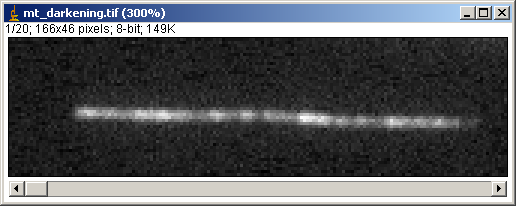
\includegraphics[scale=0.6]{fig/fig23441_mtStack.png}
\caption{A stack with darkening microtubule}
\label{fig:MTstack}
\end{center}
\end{figure} 

Go back to the first frame and do \ijmenu{[Image -> Adjust -> Thresholding\ldots]}. The image is then automatically adjusted with threshold level. and it seems Ok that the structure is well segmented. But the problem appears as you slid the bar at the bottom. Since image is darkening, area where highlighted decreases. 

%figure
\begin{figure}[htbp]
 \centering
 \subfloat[]{\label{fig:frame1Th}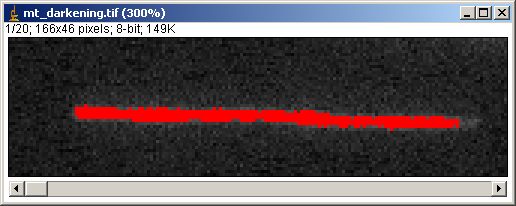
\includegraphics[height = 20mm]{fig/fig23442a_frame1threshold.png}}
 \subfloat[]{\label{fig:framelastTh}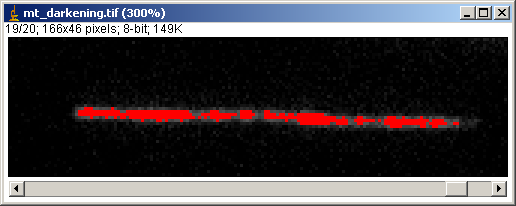
\includegraphics[height = 20mm]{fig/fig23442b_frameLastthreshold.png}}
 \caption{Adjusted with threshold level first frame (a) and the last frame (b)}
 \label{fig:degradingThreshold}
\end{figure}

This is because the threshold minimum and the maximum is kept constant while the intensity of the image is decreasing. To segment the structure while the image darkening is occurring, we must adjust the threshold intensity range as the frame progresses. 
 
The macro below finds the minimum value for the thresholding, that the highlighted area in each frame in a stack is approximately similar to the first frame. \ilcom{while} is used to loop the adjustment until the highlighted area is constant.  Then the threshold is applied to the image to convert the stack to a binary stack. 

\lstinputlisting[morekeywords={*, getThreshold, getSliceNumber, getImageID, getResult, while, setThreshold}]{code/code14.ijm}

%figure
\begin{figure}[htbp]
 \centering
 \subfloat[]{\label{fig:binMTorg}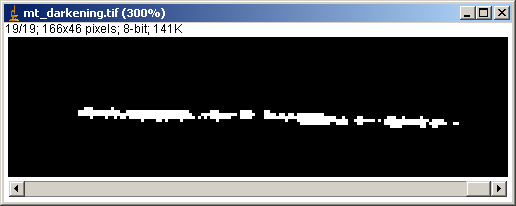
\includegraphics[height = 20mm]{fig/fig23443a_framelastbinOrg.png}}
 \subfloat[]{\label{fig:binMTproc}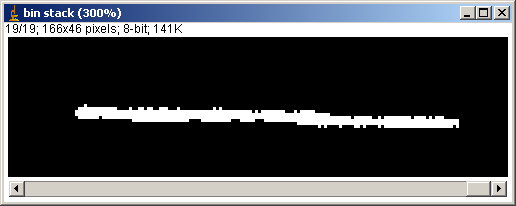
\includegraphics[height = 20mm]{fig/fig23443b_framelastbinProc.png}}
 \caption{Binarized last frame without threshold adjustment (a) and with adjustment using macro (b).}
 \label{fig:ThresholdAdjustResults}
\end{figure}

\begin{itemize}
\item Lines 3 to 5 Check if the active window is a stack. If \ilcom{nSlices==1} (meaning that the image is not a stack), macro is terminated. 

\item Lines 6 to 9: Get the threshold parameter from image and check if the image is adjusted with threshold level. If not, both upper and lower values are -1. In this case, macro is terminated. 

\item Lines 10 to 14: Get stack information. \ilcom{getSliceNumber()} returns the current frame in the stack. Adjusted with threshold level area in this frame (first frame) will be used as the reference area. \ilcom{getImageID()} returns a number that specifically identifies the active window. This ImageID will be used later,by \ilcom{selectImageID(ImageID)} to re-activate the window. 
%\end{itemize}

\begin{indentCom}
\textbf{getImageID()}\\
Returns the unique ID (a negative number) of the active image. Use the selectImage(id), isOpen(id) and isActive(id) functions to activate an image or to determine if it is open or active. 
\end{indentCom}
%\begin{itemize}
\item Line 16: clears the results table without saving. 

\item Line 17: sets the measurement parameter Area, and limits the measurement to the adjusted with threshold level region. 

\item Line 18: Do the measurements. Result is recorded in the first row of the Results table.

\item Line 19: The measured area is stored in the variable ref\_area. 

\item Line 20: temp\_area will be used later in the while loop. 

\item Line 21: the variable ilcom{tol} is a tolerance ratio of error against the reference area. So the adjusted with threshold level area in each frame should be between 97 and 103\% of the reference area. 

\item Line 22: Create a destination stack, where adjusted with threshold level images will be pasted. 

\item Line 23: get the Image ID of newly created image. 

\item Line 25: Loop for the frames starts. 

\item Lines 26, 7: Select the original stack and sets the frame number according to the loop number. \ilcom{selectImageID} works with \ilcom{getImageID} function in line 14. 


\begin{indentCom}
\textbf{selectImage(id)}\\
Activates the image with the specified ID (a negative number). If id is greater than zero, activates the idth image listed in the Window menu. With ImageJ 1.33n and later, id can be an image title (a string).
\end{indentCom}

\item Line 28: Copy the full frame.

\item Lines 29, 30: creates a temporally single frame image and the image copied in line 28 is pasted. 

\item Lines 31 to 37: While loop. temp\_area is evaluated if the area is outside 97 and 103\% of the reference area. If true, then loop continues. Initial temp\_area value is 0 so the loop is at least one time. Set Threshold with lower and upper (line 32). Measure the adjusted with threshold level area, and then lower is incremented -1. The area is evaluated, and if it does not meet the criteria set in line 31, then the loop continues with wider threshold range. 

\item Lines 38 to 40: The adjusted with threshold level image will be converted to black \& white image and then copied. The single frame temporary image is closed.

\item Line 41, 42: destination stack is activated and the same frame as the source stack is set. 

\item Line 43: Binarized image in the clipboard is pasted into the destination stack.

\item Line 44: returns to Line 25 until all stack frames are processed.

\item Line 45: Terminates the macro. 
\end{itemize}

\newpage

\section{Advanced Macro Programming}
This section could be a bit boring for you in terms of biology, but try to be patient. 
All these knowledge are required for advanced programming. 
Ability to do complex image processing using macro widens your view on planning experiments also.

\subsection{User-defined Functions}

As your code becomes longer, 
you will start to realize that similar processing or 
calculation appears several times in a macro or through macro sets. 
To simplify such redundancy, one could write a 
separate \ilcom{function} that works as a module for macros. 
For example, if you have a simple code like:
\lstinputlisting[morekeywords={*,}]{code/code15.ijm}
It should be easy for you to expect that this macro will print out "3" in the Log window. 
From this macro, we could extract part of it and make a separate function. 
\lstinputlisting[morekeywords={*,}]{code/code15_1.ijm}
This is not a macro, but is a program that works as a unit. 
Functions can be embedded in macro. \ilcom{ReturnAdd }(code 15.1) is the name of the function, 
and the following \ilcom{(n, m)} are the variables that will be used in the function. Within the function, 
n and m will be added and the result of which is substituted in to a new variable p. 
\ilcom{return p} in line 4 will return a value as an output of the function. 
We call such custom-made function as ``user-defined function''. Using this function, code 15 can be rewritten as
\lstinputlisting[morekeywords={*,}]{code/code15_2.ijm}
or simpler, by nesting the custom made function inside ImageJ native function \ilcom{print()},
\lstinputlisting[morekeywords={*,}]{code/code15_3.ijm}
Macro interpreter reads the macro line by line. When the interpreter sees \ilcom{ReturnAdd(a, b)}, 
the interpreter first tries to find the function within the ImageJ Build-in function. 
If its not there, the interpreter looks for the function within the same macro file\ldots 
(user-defined function (e.g. \ilcom{ReturnAdd(a, b)} must be written in the same macro file. 
Here is how it looks like: a macro that uses a function. 
%figure
\begin{figure}[htbp]
\begin{center}
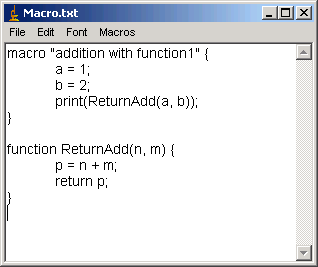
\includegraphics[scale=0.6]{fig/fig2411_usingFunction.png}
\caption{A macro file with function}
\label{fig:MacroWithFunction}
\end{center}
\end{figure} 

In this simple case, 
you might not feel the convenience of the user-defined function, 
but you will start to feel its power as you start writing longer codes. 
Advantages of using \ilcom{function} are
\begin{enumerate} 
\item Once written in a macro file, it could be used as a single line function 
as many times as you want in the macro file. This also means that if there is a bug, 
fixing the function solves the problem in all places where the function is used.
\item Long codes could be simplified to an explicit outline of events. Such as:
\begin{lstlisting}[numbers=none]
macro "whatever" {
    	function1;
		function2;
		function3;
}
\end{lstlisting}
\end{enumerate}

Let's go back to the code 14, the automatic threshold adjusting macro. 

At the beginning of the code, we check if the active image if it is a stack. 
There is another check after that, to see if the image is adjusted with threshold level.

\lstinputlisting[linerange={1-10}]{code/code14.ijm}

We can make a function for checking stack (line 3 to 5) and another function that checks 
if the stack is adjusted with threshold level (from line 6 to 9) as below.

\lstinputlisting{code/code16_17functions.ijm}

Then the initial part of code 14 (line 3 to 9) can now be replaced with 
these two functions\footnote{For a complete coding of 14.1, 
getThreshold(lower, upper) should appear again in line 8 to get lower and upper threshold value 
of the reference image.}. 

\lstinputlisting[linerange={1-5}]{code/code14_1.ijm}

\begin{indentexercise}{1}
The following macro asks the user to input x and y coordinates of two points, 
calculate the distance between those points and prints out the distance. 
Modify the code so that the distance calculation is done in a separate function. 

\lstinputlisting{code/code18.ijm}

Note that function \ilcom{pow()} in the code is defined as
\begin{indentCom}
\textbf{pow}(base, exponent)\\
Returns the value of base raised to the power of exponent. 
\end{indentCom}
For example, \ilcom{pow(4, 2)} returns 16.
\end{indentexercise}

\subsection{Multi-parameter dialogue}
In code 18 we examined above, 
user-interface is very poor since before calculation the user must input\ldots 
click\ldots input\ldots click\ldots for total of four times. 
To ease this exhausting series of input process, 
you could create a dialog box that asks the user to input several parameters at once. 
We use \ilcom{Dialog} functions. 

\lstinputlisting[morekeywords={*, Dialog, create, addMessage, addNumber, addCheckbox, show, getNumber, getCheckbox}]{code/code18_5.ijm}

%figure
\begin{figure}[htbp]
\begin{center}
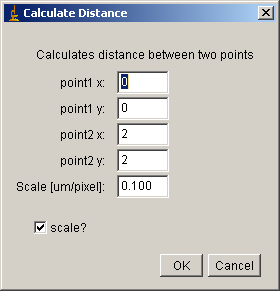
\includegraphics[scale=0.6]{fig/fig2421_GenDialog.png}
\caption{Custom Parameter Input Dialog}
\label{figGenericDialog}
\end{center}
\end{figure} 

Line 2 to 9 creates a dialog box that has multiple input boxes that looks like Fig. \ref{figGenericDialog}. 

\begin{itemize}
\item Line 3 defines the title of the dialog window. 


\item Line 4 texts will be shown within the window. 

\item Line 5 to 11 defines the parameter input fields. Fields appear in the dialog box in the order of lines with Dialog.addNumber function in the macro. When you press OK button in the dialog box, parameter will be stored in the same order. 

\item Line 15 to 19 These values then are assigned to each variable by Dialog.getNumber(). 

\item Line 20 Checkbox is independent from these number fields and the value is returned by \ilcom{Dialog.getCheckbox()}. When you check the check box, the return value is 1. If not, the return value is 0. We use this Boolean value (true or false)  to decide if the scale will be multiplied to the distance [pixel] in Line 24.

\item Line 24 This if-statement does not have braces. Such simplification is possible if there is one line when "if" is true.  
\end{itemize}

You may also realize that the if statement in line 24 (and also in Line 28) does not have comparison like == or <  or so on. This is because \ilcom{switchscale} takes only 0 or 1 (\textbf{boolean}), which are interpreted as true ( \ilcom{switchscale} = 1) or false ( \ilcom{switchscale} = 0). So even without comparison, \ilcom{switchscale} is already a decision.  

\begin{indentexercise}{1}
Modify Code 5 so that two parameters are asked in a single dialog box. 
\end{indentexercise}

\subsection{Global Variables}

"Global variables" are variables that are defined outside macro or function within the same macro file. So what is good about Global variables? For instance in Code 18.5, we had a variable called \ilcom{scale}. \ilcom{scale} had to be typed every time when you execute the macro. One way to avoid such tedious interaction with the program is forget about the line 10 and 19, where the user input is asked for the \ilcom{scale}, and instead place something like
\begin{lstlisting}[numbers=none]
scale = 0.1
\end{lstlisting}
somewhere at the beginning of the macro. This works OK, but the problem appears 
when there are many macros in the file, since it will be a loads of work to 
find the variable \ilcom{scale} in the file and change the value. 
It could also be that the name of variable is not \ilcom{scale} and something like \ilcom{pixelsize}, 
which then you have to check what this variable is doing. Furthermore, 
it becomes redundant if you need to calculate the scale in every macro. 
For this reason, you could define the scale only once in the macro file such that:

\lstinputlisting[linerange={1-20}, morekeywords={*, Gscale}]{code/code18_75.ijm}

\ilcom{var} is a statement that tells macro interpreter to treat the variable as a global variable. 
It should be always outside the scope (braces) of macro or function. 
I replaced the default value in the scale input field of the \ilcom{dialog.addnumber()} at line 11 
to \ilcom{Gscale}, so that the initial value defined in line 2 appears in the dialog box. 
The value in the field could be modified by the user, 
but this does not affect the \ilcom{Gscale} value defined in Line 2. 
This is because the flow of information is:

\ilcom{Gscale} \\
\tab > default value for the \ilcom{Dialog.addNumber} field 5 \\
\tab\tab > user changes the value  \\
\tab\tab\tab > stored in the \ilcom{Dialog.addNumber} field 5\\
\tab\tab\tab\tab > scale = \ilcom{Dialog.getNumber} (field 5)\\

So \ilcom{Gscale} is referenced, but not modified. 
If you want to change the Global value from inside the macro, you must redefine by such as
\begin{lstlisting}[numbers=none]
Gscale = scale;
\end{lstlisting}
In the macro set below, we test the use of global variable (+ function!). 
The macro is for the conversion of pixel length into micrometer. 
The second macro changes the scale value. 
I usually put G for all global variable. This is not necessary, 
but in a file with many macros this is convenient.
\lstinputlisting[morekeywords={*, G_scale}]{code/code19_globalVariable.ijm}
\begin{indentexercise}{1}
Add another global variable G\_scale\_z ( [\ensuremath{\mu}m]) for storing spacing in z-axis. 
Change the first macro, that it calculates the size of Voxel in um3. 
Then add another macro for changing the scale in Z axis. 
\end{indentexercise}

\subsection{String Arrays}
Array is a powerful tool. before going into how to use it, here is an easy explanation. 
Imagine that an array is a stack of boxes. Boxes could contain either numbers or strings. 
For instance, if you have a following list of strings:

\textit{Heidelberg, Hamburg, Hixton, Grenoble, Monterotondo}

An array "EMBL" could be prepared and each array element could contain one of these five strings. 

 %figure
\begin{figure}[htbp]
\begin{center}
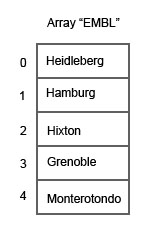
\includegraphics[scale=0.6]{fig/fig2441_arrayScheme.jpg}
\caption{EMBL array}
\label{figEMBLarray}
\end{center}
\end{figure} 
 
Then when you want to retrieve some name from the array, you refer to the address within the array. 
So EMBL[0] will be Heidelberg, EMBL[4] will be Monterotondo, and so on. 
In such a way, files names contained in a folder could be listed and stored, 
or x-y coordinates of free-hand ROI could be stored for further use. 

Here is a macro using the EMBL array example. 

\lstinputlisting[morekeywords={*, newArray}]{code/code20.ijm}

\begin{itemize}
\item Line 3 uses a function that creates a new array (\ilcom{newArray()}),
defined by a parameter for number of array elements (in the example case its 5) and its name \ilcom{EMBL}.
\item From line 4 to 8, each array from position 0 to 4 will be filled with
names (Array starts with 0th element).
\item Line 9 asks the user to input the address (position) within the array.
Then this input address is examined if the address exists within the
\ilcom{EMBL} array in line 10. \ilcom{EMBL.length} returns the number of "boxes"
within the array. If this is satisfied, then line 10 prints out the string in that address.
\end{itemize}

Array could be created and initialized with actual values at the
same time, so line 3 to 8 could be written in a single line like this: 
\begin{lstlisting}[numbers=none]
EMBL = newArray("Heidelberg","Hamburg","Hixton","Grenoble","Monterotondo");
for (i = 0; i < EMBL.length; i++)
    print(EMBL[i]);
\end{lstlisting}

\subsection{Numerical Array}

Array could also contain numerical values, and this way of usage is more common when you do image analysis. Here is a simple example of numerical array that prints out intensity profile along selected line ROI. 

\lstinputlisting[morekeywords={*, newArray, selectionType, getProfile, setResult, updateResults}]{code/code20_5.ijm}

\begin{itemize}
\item Line 3: Check if the selection type is a straight line ROI. If not, macro terminates leaving a message. 

\begin{indentCom}
\textbf{selectionType}()\\ 
Returns the selection type, where 0=rectangle, 1=oval, 2=polygon, 3=freehand, 4=traced, 5=straight line, 6=segmented line, 7=freehand line, 8=angle, 9=composite and 10=point. Returns -1 if there is no selection.
\end{indentCom}

\item Line 4: Empty array \ilcom{tempProfile} is loaded with the intensity profile along the line ROI by \ilcom{getProfile}().
\item
\begin{indentCom}
\textbf{getProfile}()\\
Runs \ijmenu{[Analyze > Plot Profile]} (without displaying the plot) and returns the intensity values as an array.
\end{indentCom}

\item Line 5: Passing the array \ilcom{tempProfile} to function "output\_results", which prints the content of array in the table shown in the ``Results'' window. 

\item Line 7 to 14: A function for outputting the profile array in the table shown in the ``Results'' window. It takes an argument \ilcom{rA}, which is supposed to be an array. 
\item Line 8: Clears the results table. 
\item Line 9 to 12: for-loop to go through the array and to print out each element. 
\item Line 10: Sets the pixel position along the segment in the column labeled "n". 
\item Line 11: Sets the content of the array (pixel intensity) in the column labeled "intensity".

\begin{indentCom}
\textbf{setResult}("Column", row, value)
Adds an entry to the ImageJ results table or modifies an existing entry. The first argument specifies a column in the table. If the specified column does not exist, it is added. The second argument specifies the row, where 0<=row<=nResults. (nResults is a predefined variable.) A row is added to the table if row=nResults. The third argument is the value to be added or modified. 
\end{indentCom}
\item Line 13: Updates the table shown in the ``Results'' window. 

\begin{indentCom}
\textbf{updateResults}()
Call this function to update the "Results" window after the results table has been modified by calls to the setResult() function. 
\end{indentCom}
\end{itemize}

\begin{indentexercise}{1}
Modify code 20.5 that the macro calculates the sum of all intensities.\\

Hint:

\begin{itemize}
\item
\item You do not need the function anymore. 
\item \ilcom{for}-loop should be used.
\item Use \ilcom{tempProfile.length}
\end{itemize}
\end{indentexercise}

\subsection{Array Functions}

Arrays could be directly treated using array functions. These functions are:
\begin{shaded}\begin{indentCom}
\item \textbf{Array.concat(array1,array2)} Returns a new array created by
joining two or more arrays or values. 
\item \textbf{Array.copy(array)} Returns a copy of array. 
\item \textbf{Array.fill(array, value)} Assigns the specified numeric value to
each element of array.
\item \textbf{Array.findMaxima(array, tolerance)} Returns an array holding the peak positions (sorted with descending strength). Tolerance is the minimum amplitude difference to needed to separate two peaks. There is an optional 'excludeOnEdges' argument that defaults to 'true'. Examples. Requires 1.48c.
\item \textbf{Array.findMinima(array, tolerance)} Returns an array holding the minima positions. Requires 1.48c.
\item \textbf{Array.fourier(array, windowType)} Calculates and returns the Fourier amplitudes of array. WindowType can be "none", "Hamming", "Hann", or "flat-top", or may be omitted (meaning "none"). See the TestArrayFourier macro for an example and more documentation. Requires 1.49i. 
\item \textbf{Array.getStatistics(array, min, max, mean, stdDev)} Returns the
min, max, mean, and stdDev of array, which must contain all numbers.
\item \textbf{Array.print(array)} Prints the array on a single line. 
\item \textbf{Array.rankPositions(array)} Returns, as an array, the rank
positions of array, which must contain all numbers or all strings. 
\item \textbf{Array.resample(array,len)} Returns an array which is linearly resampled to a different length. Requires 1.47j. 
\item \textbf{Array.reverse(array)} Reverses (inverts) the order of the
elements in array. 
\item \textbf{Array.show(array)} Displays the contents of array in a window. Requires 1.48d.
\item \textbf{Array.show("title", array1, array2, ...)} Displays one or more arrays in a Results window (examples). If title (optional) is "Results", the window will be the active Results window, otherwise, it will be a dormant Results window (see also IJ.renameResults). If title ends with "(indexes)", a 0-based Index column is shown. If title ends with "(row numbers)", the row number column is shown. Requires 1.48d. 
\item \textbf{Array.slice(array,start,end)} Extracts a part of an array and
returns it. 
\item \textbf{Array.sort(array)} Sorts array, which must contain all numbers
or all strings. String sorts are case-insensitive in v1.44i or later.
\item \textbf{Array.trim(array, n)} Returns an array that contains the first n
elements of array.
\end{indentCom}\end{shaded}

For example, array could be sorted and reversed:

\begin{lstlisting}[numbers=none]
EMBL = newArray("Heidelberg","Hamburg","Hixton","Grenoble","Monterotondo");
Array.print(EMBL);
Array.sort(EMBL);
Array.print(EMBL);
Array.reverse(EMBL);
Array.print(EMBL);
\end{lstlisting} 
The output of this code is:
\begin{lstlisting}[numbers=left]
Heidelberg,Hamburg,Hixton,Grenoble,Monterotondo
Grenoble,Hamburg,Heidelberg,Hixton,Monterotondo
Monterotondo,Hixton,Heidelberg,Hamburg,Grenoble
\end{lstlisting} 
The first line is printed in the order when the array was initialized. After
sorting, names are in alphabetical order. Third line shows the reversed
elements. 

\subsection{Application of Array in Image Analysis}
\subsubsection{Build-in Macro Functions using Array}

Many built-in macro functions return an array, to have multiple numerical values as a singular object. Below is a list of those array-returning functions. 

\begin{indentCom}
\texttt{
\item Dialog.addChoice("Label", items) 
\item Dialog.addChoice("Label", items, default)
\item Fit.doFit(equation, xpoints, ypoints)
\item Fit.doFit(equation, xpoints, ypoints, initialGuesses)
\item getFileList(directory)
\item getHistogram(values, counts, nBins[, histMin, histMax])
\item getList("window.titles")
\item getList("java.properties")
\item getLut(reds, greens, blues)
\item getProfile()
\item getRawStatistics(nPixels, mean, min, max, std, histogram)
\item getSelectionCoordinates(xCoordinates, yCoordinates)
\item getStatistics(area, mean, min, max, std, histogram)
\item makeSelection(type, xcoord, ycoord)
\item newArray(size)
\item newMenu(macroName, stringArray)
\item Plot.create("Title", "X-axis Label", "Y-axis Label", xValues, yValues)
\item Plot.add("circles", xValues, yValues)
\item Plot.getValues(xpoints, ypoints)
\item setLut(reds, greens, blues)
\item split(string, delimiters) 
}
\end{indentCom}

\subsubsection{Accessing Intensity Profile}

To learn the actual use of Array in Image analysis, we explore several example applications. The first is to try using \ilcom{getProfile} function to access intensity profile from macro. 

%\begin{indentCom}
%\fbox{
%\parbox[b][8em][c]{0.80\textwidth}{
\begin{shaded}\begin{indentCom}
\textbf{getProfile()}\\
Runs Analyze>Plot Profile (without displaying the plot) and returns the intensity values as an array. For an example, see the GetProfileExample macro\footnote{\url{http://rsb.info.nih.gov/ij/macros/GetProfileExample.txt}}. See also: Plot.getValues().
\end{indentCom}\end{shaded}
%}
%}
%\end{indentCom}
 
We create a macro that reads the line-profile from a segmented line ROI. Get an array of pixel values along this segmented ROI using the \ilcom{getProfile} function, and then mean intensity and the standard deviation of the values will be calculated and printed. 
Before running the macro code20\_3.ijm, an image (could be anything) with segment ROI selected should be the active image (fig. \ref{fig:segmentedROIselected}). 

\lstinputlisting[morekeywords={*, getProfile, Array, , print, getStatistics}]{code/code20_3.ijm}


\begin{figure}[h!]
\begin{center}
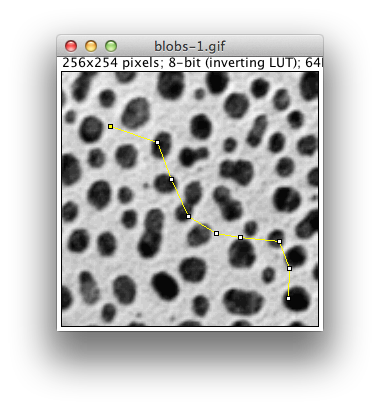
\includegraphics[width=0.5\textwidth]{fig/segmentROIselected.png}
\caption{An image with segmented ROI}
\label{fig:segmentedROIselected}
\end{center}
\end{figure}

\begin{itemize}
\item line3:  Check if the selection type is a straight line ROI using function \ilcom{selectionType}. If not, macro terminates leaving a message.
\begin{indentCom}
\fbox{
\parbox[b][8em][c]{0.80\textwidth}{
\textbf{selectionType()}\\
Returns the selection type, where 0=rectangle, 1=oval, 2=polygon, 3=freehand, 4=traced,
     5=straight line, 6=segmented line, 7=freehand line, 8=angle, 9=composite and 10=point.
     Returns -1 if there is no selection.
}
}
\end{indentCom}
\item Line 4: Empty array \ilcom{pA} is loaded with the intensity profile along the segment ROI by \ilcom{getProfile}().
\item Line 5: This line is not necessary, just to print out the array contents in the log window. 
\item Line 6: Does the array statistics.  \ilcom{min, max, mean, stdDev} will be the variables to be loaded with the results of calculating statistics. 
\item Line 7: Prints out the result of line 6 in the log window. 
\end{itemize}


\begin{indentexercise}{1}
\item Add some codes that the macro also prints out the total intensity along the segment ROI. Use looping. \\
\end{indentexercise}

\subsubsection{Extending Stack Analysis by Direct Measurements}

We studied how to use for-loops to measure each frame/slice within a stack (\ref{sec:forloopStack}). There we did measurements by firstly setting measurement parameters with \ilcom{run("Set Measurements...")} and then did measurement by \ilcom{run("Measure")}. Measured values were shown in the table in the ``Results'' window. To use those measured values to \textit{e.g.} calculate statistics or plot the results, one should access the table in the ``Results'' window and parse all the values. This is possible with the macro language, but we will not try this method as it is indirect. Instead, we try to access directly to the measured values and compute. There are two ways. 

\begin{enumerate}
\item \ilcom{getRawStatistics(nPixels, mean, min, max, std, histogram)}
\item \ilcom{List.setMeasurement}
\end{enumerate}
The function \ilcom{getRawStatistics} measures statistical parameters from the image and returns those values in the variables declared as arguments. In other words, after having this command, variable \ilcom{mean} will have the mean intensity of the image
\footnote{In this example we used a variable named \ilcom{mean}, but the name could be anything such as \ilcom{a} or \ilcom{b}.}. 
If a ROI is selected, mean intensity of that ROI will be the value of \ilcom{mean}. We could loop each slice/frame within a stack and for each loop we could do \ilcom{getRawStatistics} and store measured values in arrays. This is doable, but has a drawback of using this function: the available parameters to measure is limited. 

The second method \ilcom{List.setMeasurement} does not have this limitation. One could measure many more parameters because all the available parameters in \ilcom{[Analyze > Set Measurements...]} are accessible with this function. The basic usage is shown below.

\begin{lstlisting}
List.setMeasurements;
mean = List.getValue("Mean");
print(mean)
\end{lstlisting}

This code measures the currently active image, extracts specific measurement value (in the above case ``Mean'' intensity) and then prints out that value in the log window. We could do this measurement for every loop for stack slices/frames and store the results in arrays. Here is the code, a modified version of code 10. 

\lstinputlisting[morekeywords={*, List, setMeasurements, getValue, newArray}]{code/code10_1.ijm}
\begin{itemize}
  \item Line 2: Checks the ImageJ version, since \ilcom{List.setMeasurements} function is only available after version 1.42i.
  \item Line 5, 6: Create new arrays with their length same as the number of frames within the stack. These arrays will be used to store measurement results. 
  \item Line7: for-loop going through each frames in the stack.
  \item Line 10: Do measurement. All the parameters will be stored in the List. 
  \item Line 11, 12: Retrieve the results, mean intensity and standard deviation. 
  \item Line 15, 16: Print out results in the log window. 
\end{itemize}

\subsubsection{Acquiring intensity profile from segmented line ROI}
 
In recent version of ImageJ, selection thickness controls the width of segmented
line ROI when you do \ijmenu{[Analyze > Plot Profile])}. We try to mimick this
behavior in macro, and instead of choosing the line ROI thickness using GUI, the
macro asks the user to input the thickness. 

In the code below, there is only one macro. Two functions are added at the
bottom. One is for profile plotting and the last one is for listing
intensity profile data in the result table. Strategy of this macro is to use
straight line selection for each segment, measure that segment and then profiles
are concatenated to the total profile array.

%\lstinputlisting[morekeywords={*, newArray, selectionType, getProfile, setResult, updateResults}]{code/code20_75.ijm}
%\lstinputlisting[morekeywords={*, getSelectionCoordinates, makeLine, Plot,
% create, setLimits, setColor, add, show}]{code/code20_75.ijm}
\lstinputlisting[morekeywords={*, getSelectionCoordinates, makeLine, Plot,
create, setLimits, setColor, add, show, Array, concat,
getStatistics}]{code/code20_76.ijm}

\begin{itemize}
\item Lines 2 - 16: Main part, macro for the segmented line ROI measurement.  

\item Line 3: Check if the selection type is a segmented line ROI. If not, macro
terminates leaving a message.

\item Line 4: Reads the x and y coordinates of the segmented line
and store them in two arrays \ilcom{xCA} and \ilcom{yCA}.

\begin{indentCom}
\textbf{getSelectionCoordinates(xCoordinates, yCoordinates)}\\
Returns two arrays containing the X and Y coordinates of the points that define the current selection. 
\end{indentCom}

\item Line 5 - 7: Asks the user to input width of the segmented ROI. The ROI
line width is set to that value.

\item Line 8: A new array \ilcom{totalprofile} is created, initialized without
any element. This new array will store the profile data of full ROI.

\item Line 9 - 13: Profile measurement by placing straight line ROI,
for wach segment of the original ROI. \ilcom{makeLine} function is used for this
purpose, and \ilcom{getProfile} returns intensity profile of the corresponding
line ROI. Profile data in \ilcom{thisprofile} array are concatenated to
\ilcom{totalprofile} array using \ilcom{Array.concat}.

\begin{indentCom}
\textbf{makeLine(x1, y1, x2, y2)}\\
Creates a new straight line selection. The origin (0,0) is assumed to be the upper left corner of the image. Coordinates are in pixels. With ImageJ 1.35b and letter, you can create segmented line selections by specifying more than two coordinate, for example makeLine(25,34,44,19,69,30,71,56).
\end{indentCom}

\item Line 14: Call graph plotting function (Line 20 - 27), passing
\ilcom{totalprofile} array as an argument.

\item Line 15: call function to printout the profile array in the results window
(Lines 32 - 39).

\item Line 20 - 27: Function for plotting the intensity profile.
\item Line 21 : Use \ilcom{Array.getStatistics} function to know the minimum and
the maximum value of the array that was given as argument.
\item Line 22: Creates the window and axes of the plot. 
\item Line 23: Set the range for x and y axis using the results of line 21
\ilcom{min} and \ilcom{max}. 5\% of offset is added to both values for some
margins below and above.
\item Line 24: Sets the color of the plot. 
\item Line 25: Plot the profile. 
\item Line 26: Show the plot on the screen (lot is hidden until this show()
function).

\item Line 30 - 37: Function for outputting the profile array in the result
table. This function is exactly the same function you already used in the
previous chapter (code 20.5).

\end{itemize}

\newpage

\section{File I/O}

Analysis of images requires both input and out put: input is to load images, 
and output is  to save either processed images or numerical data. 
If number of image files or quantity data is manageable by manual loading and saving, 
we do not have to automate. But in some cases you need to process a huge number of files. 
This often happens especially after you establish a protocol and you want to get 
statistically sufficient amount of data. Then you need to automate file input and output using macro. 
Once you learn how to write File I/O program, you can process as much files as you want, 
as long as your memory space allows.

\subsection{Saving the Measurement Results Automatically}

When you have a time series sequence and you want to measure multiple signals with 
multiple parameters in each frame, measurement results in each frame needs to be somehow saved. 
Here, we learn how to export measurement results in your hard disk automatically using macro. 

Open the sample image \ilcom{Nucseq001.tif}. Cell nucleus shows that they divide and 
increase their number over time. We want to count the number of nucleus in each frame to know 
the dynamics of increase. 
At the same time, we may also want to see changes in the signal intensity and shape. 
For this measurement Particle Analysis function works best. Do the following:

\begin{enumerate}
\small{
\item \ijmenu{[Image -> Adjust -> Threshold]}. 
Threshold the image and check the threshold lower and upper value that segments the nucleus optimally. 
\item Set the measurement parameters. \ijmenu{[Analysis -> set measurements\ldots]}
\begin{enumerate}
\item Check Area, Mean intensity, centroid, Circularity and Slice number. 
\item Check "limit to threshold"
\item Digits after decimal point: 2
\end{enumerate}
\item \ijmenu{[Analyze -> Analyze Particles\ldots]}
\begin{enumerate}
\item Size: 10 - Infinity
\item Circularity = 0.5 - 1.0
\item Show: Outline
\item Check Display Results
\item Check Exclude on Edges
\item Check Clear Results
\end{enumerate}
\item Then click "OK". 
}
\end{enumerate}
After these steps, you will find outline image showing detected cells and a result table. 

%double figure
\begin{figure}[htbp]
 \centering
 \subfloat[]{\label{fig:thresholdCells}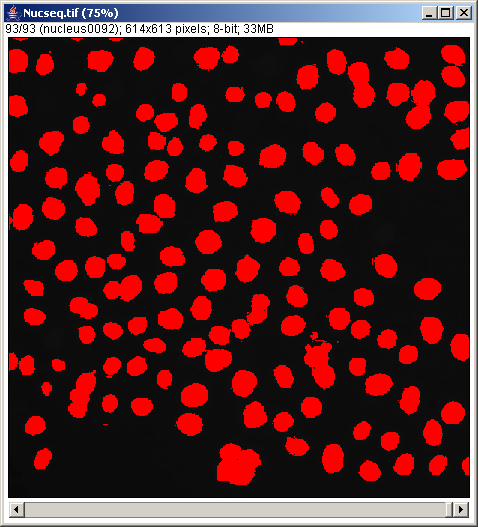
\includegraphics[height = 60mm]{fig/fig2511a_CellsThreshold.png}}
 \subfloat[]{\label{fig:ParticleAnalysisDialog}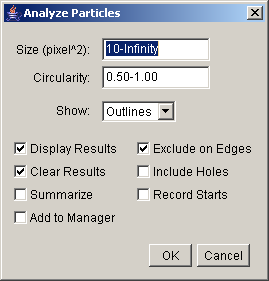
\includegraphics[height = 60mm]{fig/fig2511b_AnalyzeParticleDialog.png}}
 \caption{ (a) Thresholded cell image and (b) Particle Analysis parameter input dialog.}
 \label{fig:ParticleAnalysis}
\end{figure}

%double figure
\begin{figure}[htbp]
 \centering
 \subfloat[]{\label{fig:OutlinedCells}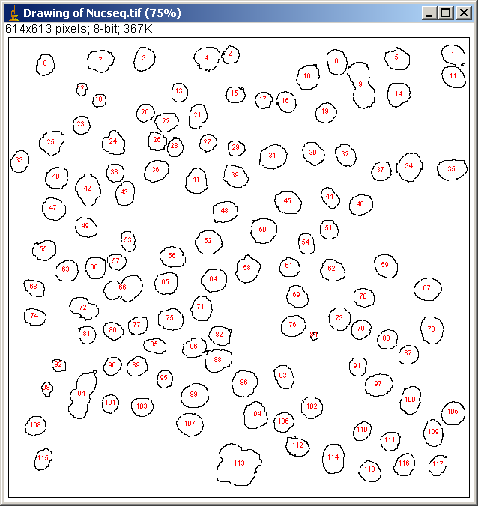
\includegraphics[height = 50mm]{fig/fig2511c_CellOutlines.png}}
 \subfloat[]{\label{fig:ParticleAnalysisResults}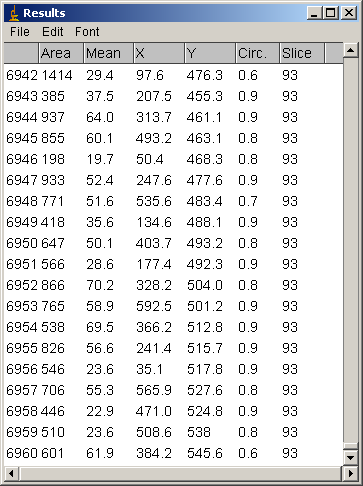
\includegraphics[height = 50mm]{fig/fig2511d_ParticleAnalysisResults.png}}
 \caption{ After particle analysis is done, (a) outlined cell image and (b) results table listing measurement results.}
 \label{fig:ParticleAnalysisResults}
\end{figure}

Using macro recorder, its easy to write a macro set as following. 

\lstinputlisting[morekeywords={*, }]{code/code21.ijm}

Two macros and a global variable consists this macro set. 
Global variable is a string variable that stores the path to the location where file will be saved. 
(note: path is differently written in MacOS. It uses slash instead of back-slash). 
The first macro \ilcom{Set Directory to save Results} is for setting the path to the folder 
(or directory) where the file will be saved. 
We use a macro function \ilcom{getDirectory(title)} to get user choice of a destination folder. 

\begin{indentCom}
\textbf{getDirectory(title)}\\
Returns the path to a specified directory. If title is "startup", returns the path to the directory 
that ImageJ was launched from (usually the ImageJ directory). If it is "plugins" or 
"macros", returns the path to the plugins or macros folder. If it is "image", 
returns the path to the directory that the active image was loaded from. 
If it is "home", returns the path to users home directory. 
If it is "temp", returns the path to the /tmp directory. 
Otherwise, displays a dialog (with title as the title), 
and returns the path to the directory selected by the user. 
Note that the path returned by getDirectory() ends with a file separator, 
either "\" (Windows) or "/". Returns an empty string if the specified directory is not found or 
aborts the macro if the user cancels the dialog box.
\end{indentCom}

When you run this first macro, global string variable \ilcom{G\_Ddir} 
will be set to a folder where user will select, and line 6 prints out the path to 
a folder (or directory). It might be convenient for you to change the default directory path 
in the code above (line 2), by copying the results in the log window and pasting it in the macro. 

The measurement macro starts from the Line 9. 
\begin{itemize}
\item Line 10 to 13: Checks if the image is thresholded. 
\item Line 14: Sets the threshold level. 
\item Line 15: Gets the title of the image window for later use. We use this for 
generating name of the results file.
\item Line 16: to 17: Sets the measurement parameter and does the actual 
particle analysis. Macro functions are direct copies from the recorder. 
\end{itemize}
After the analysis, we want to save the results. 
\begin{itemize}
\item Line 18: Generates the file name using the image file name stored in the line 15 by concatenating concatenate image title with \ilcom{\_measure.xls}. 
\item Line 19: The full path file name is constructed by adding the result filename generated in line 18 with path stored in the global variable. 
\item Line 20: Saving the result table as an excel-readable file uses a new macro function \ilcom{saveAs}:
\begin{indentCom}
\textbf{saveAs(format, path)}
Saves the active image, lookup table, selection, measurement results, selection XY coordinates or text window to the specified file path. The format argument must be "tiff", "jpeg", "gif", "zip", "raw", "avi", "bmp", "fits", "png", "pgm", "text image", "lut", "selection", "measurements", "xy Coordinates" or "text". Use saveAs(format) to have a "Save As" dialog displayed.
\end{indentCom}
Path in line 20 is a full path constructed in the previous line 19.
\end{itemize}

\begin{indentexercise}{1}
Create a new macro file and write the code 21. If it works, save the macro as "macro\_fileIO.ijm". We use it in the next section (.ijm is the extension for imageJ macro). 
Then modify the code so that user can change the size-range for the particle analysis. Save the file separately.   
\end{indentexercise}

\subsection{Batch Processing of Files}

What should we do if we have more stacks that should be analyzed? Should we open each of the stack and execute the macro? A better idea is to automate the loading process also. For this, we modify and extend the code written in the previous section. The tasks are:

\begin{itemize}
\item task a: List files in a folder.
\item task b: Open a file, do analysis, save results and close the file. 
\item task c: Do this until all files are analyzed.
\end{itemize}
 
A very useful function for task a is \ilcom{getFileList(path)}.
\begin{indentCom}
\textbf{getFileList(directory)}\\
Returns an array containing the names of the files in the specified directory path. The names of subdirectories have a "/" appended.
\end{indentCom}
 
You need to set the path to the source image containing folder (directory). We learn this macro function in the following short macro. 

\lstinputlisting[morekeywords={*, getDirectory, getFileList}]{code/code22.ijm}

Run this macro and if you choose a folder in the sample image folder containing four stacks,  macro prints out texts in Log window. It should then look like figure \ref{fig:code22out}.
%figure 
\begin{figure}[htbp]
\begin{center}
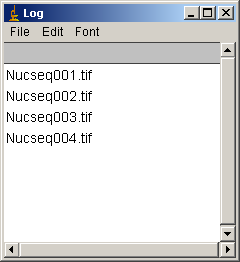
\includegraphics[scale=0.6]{fig/fig2521_FileBatchOUtput.png}
\caption{Output of code 22}
\label{fig:code22out}
\end{center}
\end{figure}

\begin{itemize}
\item Line 2: Asks the user to select a folder. Variable \ilcom{dir} is then stored with the full path to the folder. 
\item Line3 uses the \ilcom{getFileList} function, and reads out the file names as a string array and stored in List (array). 
\item Line 4 to 6 is a loop. \ilcom{list.length} returns the length of the list. In this way, all the contents are printed out in the window. 
We use this \ilcom{getFileList} function to process multiple files automatically. 
\end{itemize}

Let's modify code 22 so we can measure multiple stacks automatically. Code 23 (see below) works like this: You must first set two things: 

\begin{enumerate}
\item Full path to the destination folder where the results will be saved. 
Macro \ilcom{Set Directory to save Results}
\item Threshold level for the particle analysis. Macro \ilcom{set the threshold lower level}
\end{enumerate}

The first setting task is the same as you did in code 22. 
The second setting is done by manually opening a stack 
(may be the first one in the files) and manually setting the threshold as you like, 
then execute the second macro below. In both these settings, 
parameters will be saved in global variables and will be used in the main program. 

When you run the main macro (\ilcom{Multiple measurement}) 
after these two settings, the program asks you where the files are. 
As soon as you select a folder where files are contained, 
then processing and saving just proceeds automatically. 

\lstinputlisting[morekeywords={*, }]{code/code23_FileIO_02.ijm}

Now we have three macros and four global variables. 
\begin{itemize}
\item Line 3: global string variable for storing path to the source folder. 
\item Line 4: global string variable for storing path to the destination folder, where results will be saved. 
\item Line5 and 6: Global numerical variables for storing threshold upper and lower values. 

\item Macro \ilcom{Set Directory to save Results}: Line 9 to 12: First macro. This is used to set the path to the destination folder. The function is same as code 22.
 
\item Macro \ilcom{set the threshold lower level}: Line 14 to 20: 
This macro is for storing the lower value of the threshold in global variables, 
the values of which will be used in the main macro. You might have seen a similar code already: code 17, 
function for checking if the image is thresholded. 
Only difference is that in this code 23, 
lower threshold value is stored in the global variable defined in line 5. 
Upper value is not touched, kept to 255. 

\item Macro \ilcom{Multiple measurement}: Line 22 to 28: This is the main macro (third one in this macro set). 
Line 23 asks the user where the files are. 
This path to the source file is stored in the global variable defined in line 3. 
Then in line 24, a list of files contained in source folder is generated and stored in the array \ilcom{list}. 
From line 25 to 27 is a small for-loop, the number of loop is same as the length of the list. 
In this loop, name of file is passed one by one to the 
function \ilcom{NucAnalysis()} that does the actual analysis\ldots

\item function \ilcom{NucAnalysis(img\_filename)}: Line 30 to 51 is the core of analysis. 
\ilcom{img\_filename} is string variable for file names in the list array, given as argument. 
\begin{itemize}
\item Line 31: Using \ilcom{img\_filename},  the full path name is constructed by combining two strings. 
\item Line 32: A file is opened by \ilcom{open(path)} function. 
\begin{indentCom}
\textbf{open(path)}\\
Opens and displays a tiff, dicom, fits, pgm, jpeg, bmp, gif, lut, roi, or text file. 
Displays an error message and aborts the macro if the specified file is not in one of the supported formats, 
or if the file is not found. 
Displays a file open dialog box if path is an empty string or if there is no argument. 
Use the File>Open command with the command recorder running to generate calls to this function. 
With 1.41k or later, opens images specified by a URL.
\end{indentCom}
\item Line 33: After opening image, its \ilcom{ImageID} is stored in the variable \ilcom{sourceID}. 
\item Line 34, the image is thresholded according to the global variables for the lower and the upper values. 
\item Line 35: Title of the image, which actually is the file name, is retrieved and stored in the variable \ilcom{img\_title}. 
\item Line 38: The particle analysis is then applied to the image (Lines 34 to 37 are same as lines 14 to 17 in code 21). 
\item Line 38: Source image you opened from the hard disk is activated and then closed in line 39. 
Activation of the image by \ilcom{selectImage()} is required, 
because there is already a new stack (outline stack!), 
so that original stack is already behind. Therefore to close the original, 
one must activate the image by using \ilcom{selectImage()} function.  
\item After all these processing and measurement, results will be saved. 
Lines 42 to 45 saves the outline stack. Outline stack is also closed after saved (line 45). 
Line 47 to 50 is exactly same as the Result table saving you did in code 21 (lines 18 to 20). 
Line 49 is added, just for an additional information printout in Log window. 
\end{itemize}
\end{itemize}
\newpage


\subsection{Working with Strings}

With some advanced macro programming, you might need to manipulate Strings (texts) from your code. For example, let's think about a title of an image ``exp13\_C0\_Z10\_T3.tif''. Such naming occurs often to indicate that this image is from the third time point (T3), at the 11th slice (Z10, imagine that the Z slice numbering starts from 0) and its the first channel (C0). 

We might be lucky enough to read out its dimensional information from header, but quite often such information is only available in the file name (the title of the image). To extract dimensional information from file name, we need to know how to deal with strings in macro to decompose those strings and extract information that we need. Build-in macro functions which are related to such tasks with strings are the following. 

\begin{shaded}\begin{indentCom}
\item lengthOf(str)
\item substring(string, index1, index2)
\item indexOf(string, substring)
\item indexOf(string, substring, fromIndex)
\item lastIndexOf(string, substring)
\item startsWith(string, prefix)
\item endsWith(string, suffix)
\item matches(string, regex)
\item replace(string, old, new)
\end{indentCom}\end{shaded}

Let's go back to the example file name ``exp13\_C0\_Z10\_T3.tif'' again. If we need to get the file name without file extension, what should we do? Several ways are there, but lets start with the simplest way. 

We already know that all the file names are in the TIFF format, so all file names end with ``.tif''.  We could remove this suffix by replacing the ``.tif'' with a string with length 0. We could do this by using \ilcom{replace}. 

\begin{lstlisting}
name = "exp13_C0_Z10_T3.tif";
newname = replace(name, ".tif", "");
print(newname);
\end{lstlisting}

This will print out "exp13\_C0\_Z10\_T3" in the log window. In the second line, the function \ilcom{replace} is used. The old string ".tif" is replaced by a new 0 length string "". So it works! 

But what if our lucky assumption that all files end with ".tif" is not true and it could be anything? To work with this, we now need to use different strategy to know the file extension. 

By definition, file extension and the file name is separated by a dot. Length of the extension could be different, as some extension such as a python file is ".py" and a C code is ".c". Thus, we cannot assume that the length of the file extension is constant, but we know that there is a dot. 

For such cases with variable length of file extension being expected, we first need to know about the \textbf{index} of the dot within file name. Each character within file name is positioned at certain index from the beginning of the name. In the example we are now dealing with, the index 0 is ``e''. The index 1 is ``x''. Since the index starts from 0, the last index will be total length of the file name minus one. You could modify the code above like below to try getting the length of the file name. 

\begin{lstlisting}
name = "exp13_C0_Z10_T3.tif";
tlength = lengthOf(name);
print(tlength);
\end{lstlisting}

You should see ``19'' in the log window. That is the length of this file name. So in this example string, index starts from 0 and the last index is 18. 

Next, we use the function \ilcom{substring(string, index1, index2)}. With this function, you could extract part of the \ilcom{string} by giving the start index (index1) and the end index (index2) as arguments. We could just try this by again modifying the code above. 

\begin{lstlisting}
name = "exp13_C0_Z10_T3.tif";
subname = substring(name, 0, 3);
print(subname);
\end{lstlisting}

The output after running this code is ``exp'' printed in the log window. The second argument of the function \ilcom{substring} is 0, and the third is 3. This tells the function \ilcom{substring} to extract characters from the index 0 to the index 2 (so the third argument will be the index just after the last index that would be included in the substring). 

\begin{indentexercise}{1}
Test changing the second and the third argument so that different part of the file name is extracted. 
\end{indentexercise}

How could we know the index of the dot? For this we use the \ilcom{indexOf(string, substring)}. Try the following code. 

\begin{lstlisting}
name = "exp13_C0_Z10_T3.tif";
dotindex = indexOf(name, ".");
print(dotindex);
\end{lstlisting}

Now you know that the index of dot is ``15''. We could then combine the knowledge we have now to compose a single macro that extracts the filename without file extension. 

\begin{lstlisting}
name = "exp13_C0_Z10_T3.tif";
dotindex = indexOf(name, ".");
filename = substring(name, 0, dotindex);
print(filename);
\end{lstlisting}

Let's make the problem a bit more complicated. If the file name contains multiple dots, what should we do? In the example below, I added two more dots. 

\begin{lstlisting}
name = "exp13._C0._Z10_T3.tif";
dotindex = indexOf(name, ".");
filename = substring(name, 0, dotindex);
print(filename);
\end{lstlisting}

Output is now ``exp13''. Far from what we need. To treat such case, we use \ilcom{lastIndexOf}, which returns the index of the last appearance of the given character. Let's slightly modify the code. 

\begin{lstlisting}
name = "exp13._C0._Z10_T3.tif";
dotindex = lastIndexOf(name, ".");
filename = substring(name, 0, dotindex);
print(filename);
\end{lstlisting}

It should then working again as we want. 

Let's change our task: We now want to know the time point that this image was taken. How should we do that? Examining the file name again, we realize that the time point number appears after ``T''. The number could be any length of digits, but currently is 0. Then the dot comes right after the number. We then just need to know the index of ``T'' \ldots but wait, we might have ``T'' anywhere, as this is a single character alphabet that could easily be a file name. Therefore we find the index of ``\_T'' that looks like more specific. 

\begin{lstlisting}
name = "exp13._C0._Z10_T3.tif";
timeindex = indexOf(name, "_T");
print(timeindex);
\end{lstlisting}

Now we know that ``\_T'' is at index 14, so the number should start from the index 16 (because index 15 will be ``T''). Taken this into account, we could extract the time point. 

\begin{lstlisting}
name = "exp13._C0._Z10_T3.tif";
timeindex = indexOf(name, "_T");
dotindex = lastIndexOf(name, ".");
timepoint = substring(name, timeindex + 2, dotindex);
print(timepoint);
\end{lstlisting}

The time point that you have just now captured is a string. You can not pass this to mathematical assignments. To do so, you need to convert this to a number. For doing so, you could use \ilcom{parseInt(string)}. 

\begin{lstlisting}
name = "exp13._C0._Z10_T3.tif";
timeindex = indexOf(name, "_T");
dotindex = lastIndexOf(name, ".");
timepoint = substring(name, timeindex + 2, dotindex);
timepoint = parseInt(timepoint);
print(timepoint * 2);
\end{lstlisting}

An example case where conversion of string to number (in this case an integer) required would be when you need to compare such file names and get the maximum time point from all the file names. Usage is diverse, but at some point you need to use this. If you need a Float number (numbers with decimal point), use \ilcom{parseFloat(string)}.


\section{Secondary Measurement}
In this section we learn a macro usage which you may often encounter in actual situations: 
We do certain measurement first. We then use results from this first measurement for 
setting parameters of second measurement.  

We take following example of secondary measurement: 
\begin{enumerate}
\item We first measure XY coordinates of moving particles by particle tracking.  
\item Using these XY data, we measure changes in pixel intensity of the particle.
\end{enumerate} 
There could be two cases of how you get the data out and load it into currently running macro. 
First is to do so directly from data table within ImageJ, 
and the other is to access data file saved in hard disk. We learn both. 

\subsection{Using Values in Results Window}

ParticleTracker is an excellent plugin for automated tracking of spherical particles\footnote{ As of Nov. 2010, we have a largely updated version of ParticleTracker plugin available at the ETH site. This 2D/3D implemented version could be downloaded from ETH site \url{
http://www.mosaic.ethz.ch/Downloads/ParticleTracker}.This plugin is added with many new features but there is some bugs still. With some measurement conditions, the new plugin returns error and crashes. For this reason, please download the plugin from CMCI site for the exercise in this textbook. \url{http://cmci.embl.de/downloads/particletracker2d}.  }. We use this plugin first to get tracked data. 

\begin{indentexercise}{1}
\item Open sample image stack \textbf{TransportOfEndosomalVirus.tif}. Then do \ijmenu{[Plugins > Particle Detector \& Tracker> Particle Tracker]}. A parameter input dialog window appears. Fill in  parameters as follows:
\begin{itemize}
\item radius: 3
\item cutoff: 0
\item percentile: 0.3
\item link range: 1
\item distance: 20
\end{itemize}
\end{indentexercise}

Now, you should see a results window that looks like figure \ref{fig:particletrackingresults}.
%figure 
\begin{figure}[htbp]
\begin{center}
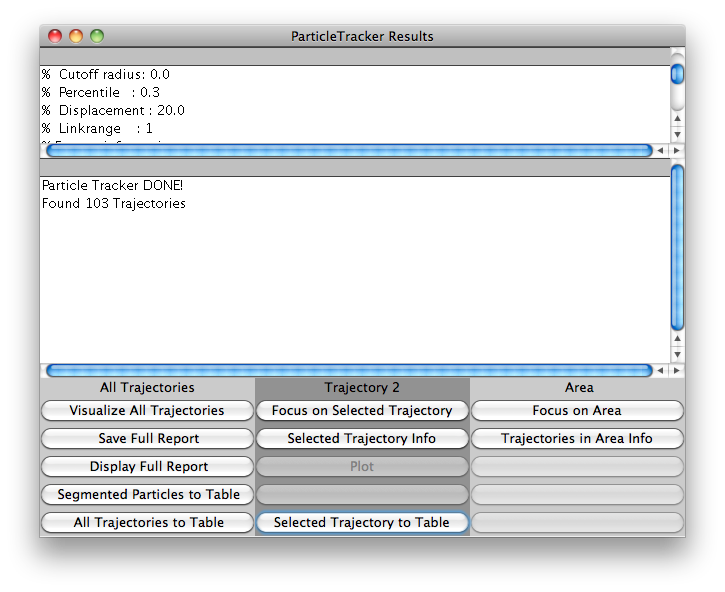
\includegraphics[scale=0.45]{fig/fig253_ParticleTrackerResults.png}
\caption{ParticleTracking Results}
\label{fig:particletrackingresults}
\end{center}
\end{figure}
In there, it should be reported that over 100 trajectories were detected. You could see how they look like by clicking "Visualize All Trajectories". 
Another window overlaid with colorful tracks appears 
(Fig. \ref{fig:particletrackingTracks}). 
Click "Filter Options" and input 10, so that short trajectories become invisible in the window. 
Use your mouse and select one of trajectory by clicking. 
Rectangle ROI is created in the surrounding of the selected track. 
Go back to the Results window (Fig. \ref{fig:particletrackingresults}) 
and click "Focus on Selected Trajectory". 
Then you will see another window is created with only the track you chose 
(Fig. \ref{fig:particletrackingTrackFocused}). 
Check carefully if the tracking was done properly. 
If you are satisfied, go back to the result window (Fig. \ref{fig:particletrackingresults}) 
again then click "selected trajectory to Table". 
You will then find the trajectory data is transferred to the Results table of ImageJ 
(Fig. \ref{fig:particletrackingTransferred}). 
 

%double figure
\begin{figure}[htbp]
 \centering
 \subfloat[]{\label{fig:particletrackingTracks}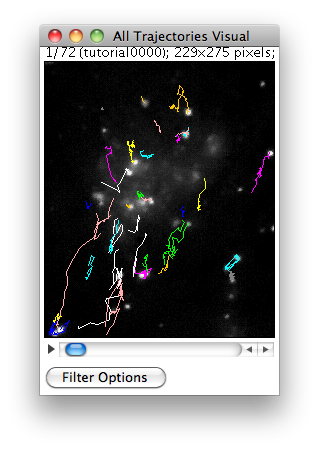
\includegraphics[height = 90mm]{fig/fig253particletrackingTracks.png}}
 \subfloat[]{\label{fig:particletrackingTrackFocused}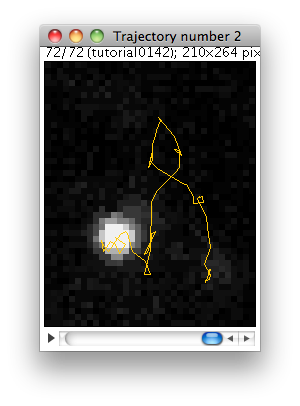
\includegraphics[height = 90mm]{fig/fig253_focusedTrajectory.png}}
 \caption{ (a) ParticleTracking Trajectories, all, and (b) Focus on Single Track.}
 \label{fig:particletrackingTrackFocused}
\end{figure}

 %figure 
\begin{figure}[htbp]
\begin{center}
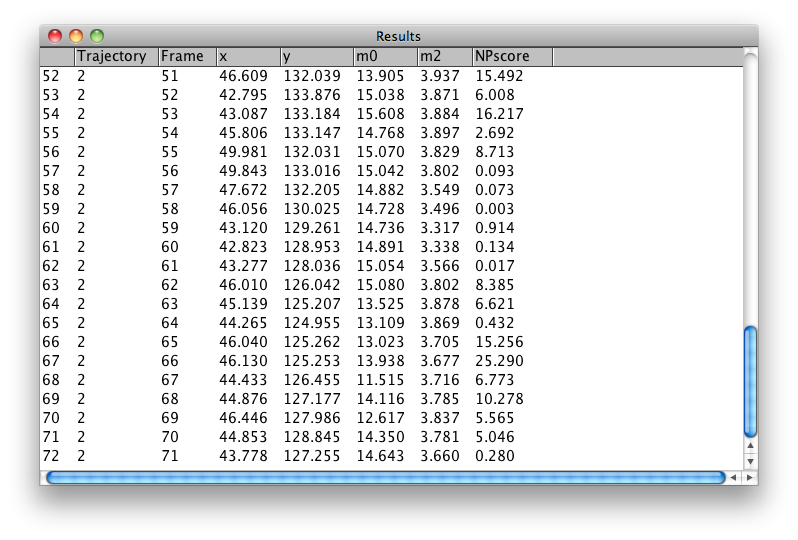
\includegraphics[scale=0.4]{fig/fig253_TrackingResultsInResultsTabel.png}
\caption{ParticleTracking Results transferred to ImageJ Results Table}
\label{fig:particletrackingTransferred}
\end{center}
\end{figure}

So now, what we have to do is access results table, 
get XY coordinates from there and do intensity measurements at corresponding positions. 
To get data out of results table, we use the following macro function:
\begin{indentCom}
\textbf{getResult("Column", row)}\\
Returns a measurement from the ImageJ results table or NaN if the specified column is not found. 
The first argument specifies a column in the table. 
It must be a "Results" window column label, such as "Area", "Mean" or "Circ.". 
The second argument specifies the row, where 0<=row<nResults. 
nResults is a predefined variable that contains the current measurement count. 
(Actually, it's a built-in function with the "()" optional.) 
Omit the second argument and the row defaults to nResults-1 (the last row in the results table). 
See also: nResults, setResult, isNaN, getResultLabel.
\end{indentCom}
Let's first test with a short macro that reads data from Results table and 
print out XY coordinates in the Log window. 

\lstinputlisting[morekeywords={*, getResult, nResults}]{code/code24.ijm}

At line 1, \ilcom{nResults} is a function that returns the number of rows in the Results table. 
Frame number is added with 1 in the line 2  because frame number in ParticleTracker plugin starts from 0, 
while it starts from 1 in ImageJ. 
In line 3 and 4, xpos and ypos is inverted, 
because ParticleTracker program was originally wrote in Matlab and for that convention 
(in Matlab, vertical diretion is called "X" and horizontal direction is called "Y", 
and this is common to matrix calculation software since row = X and column = Y), 
XY data should be inverted for use in in ImageJ. 

If you check the log window and if you are confident with data read out from Results window, 
we could now add the code with lines to measure intensity by 
placing circular ROI at XY coordinates of trajectory. Here we go. 

\lstinputlisting[morekeywords={*, getResult, makeOval}]{code/code24_5.ijm}

Running this macro, you should see a new column in Results window with header title "RoiInt", 
where measured intensity is listed (Fig. \ref{fig:PTResultsTableAfter}).

%figure 
\begin{figure}[htbp]
\begin{center}
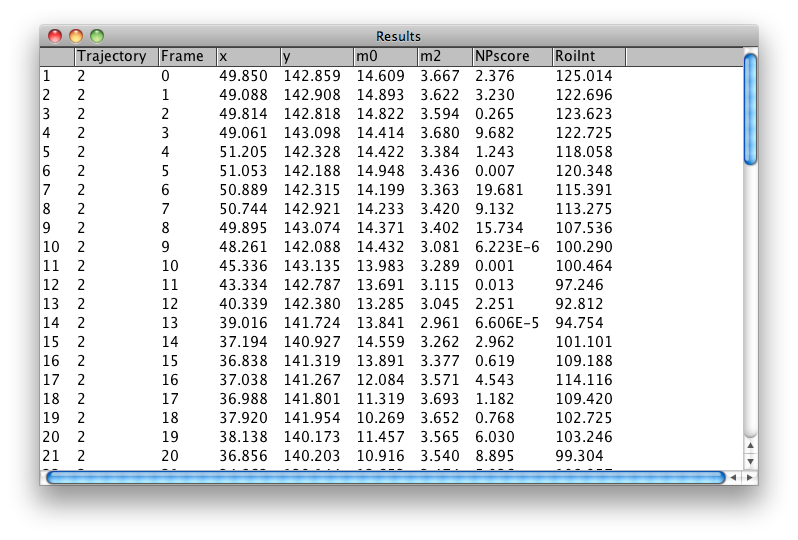
\includegraphics[scale=0.5]{fig/fig261_resultstableAddedWithInt.png}
\caption{Results Table with Intensity Measurement \\Column "RoiInt"}
\label{fig:PTResultsTableAfter}
\end{center}
\end{figure}

Explanation of the code: In the first line, 
we set the name of the image stack so that we are sure with which window to be measured with intensity. 
Line 2 and 3 are for setting the size of oval ROI. 

The way oval ROI is created is what you have learned already in detail in the section 
\ref{sec:dotmove}. \ilcom{getRawStatistics()} returns basic parameters of the selected ROI, 
and is more convenient than using \ilcom{run("Measure")}. 

\begin{indentCom}
\textbf{getRawStatistics(nPixels, mean, min, max, std, histogram)}\\
This function is similar to getStatistics except that the values returned 
are uncalibrated and the histogram of 16-bit images has a bin width of one and is returned 
as a max+1 element array. For examples, refer to the ShowStatistics macro set. 
See also: calibrate and List.setMeasurements
\end{indentCom} 

\subsection{Using values in non-Results table}
Next, we study a case when data are shown in non-Results Table. 
Manual Tracking plugin is another way of measuring particle movement, and utilizes non-Results table. 

\begin{indentexercise}{1}
Open sample image stack \textbf{TransportOfEndosomalVirus.tif} 
and track at least two virus manually\footnote{ For detailed instruction on how to use Manual tracker, 
see corresponding section in CMCI Image Processing and Analysis Course I Basic.}. 
In ImageJ, you should install this plugin by yourself. 
In Fiji, Manual Tracking plugin could be found at \ijmenu{[Plugins > tracking >]}.
\end{indentexercise}

After the tracking, we have a results table that looks like figure \ref{fig:manualtrackingresults}.
%figure 
\begin{figure}[htbp]
\begin{center}
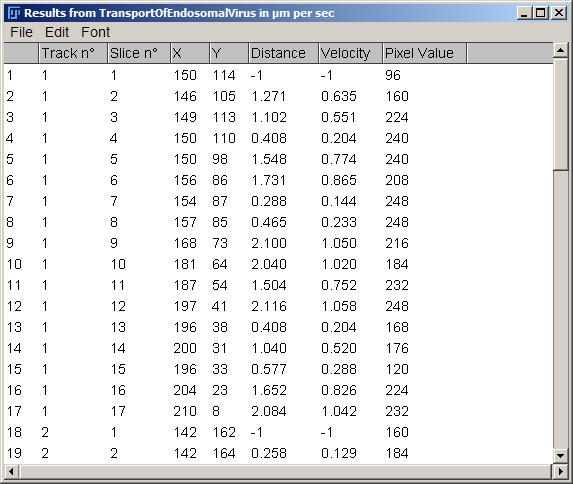
\includegraphics[scale=0.6]{fig/fig253_ManualTrackerResultsWindow.png}
\caption{Manual Tracking Results}
\label{fig:manualtrackingresults}
\end{center}
\end{figure}

To extract these data and use it for the secondary measurement, 
you might immediately think of using \ilcom{getResult(column header, row)} 
as we did in the previous subsection.

That should then be pretty straight forward\ldots 
But if you try this, you would see that this function returns error and 
does not work in case of Manual Tracking plugin. 
This is because result table created by Manual Tracking plugin is not the genuine ImageJ Results window. 
For such non-genuine results window, we retrieve data using the following function. 
\begin{indentCom}
\textbf{getInfo("window.contents")}\\
If the front window is a text window, returns the contents of that window. 
If the front window is an image, returns a string containing the text that would be displayed by 
Image>Show Info. Note that \ilcom{getImageInfo()} is a more reliable way to retrieve information 
about an image. Use \\
\ilcom{split(getInfo(),"\textbackslash{}n")} \\
to break the string returned by this function into separate lines. Replaces the \ilcom{getInfo()} function.
\end{indentCom}

This function returns a string with the content of the table. 
Try the following two lines to see how it works. \\

\begin{lstlisting}[numbers=none, morekeywords={*, getInfo}]
str = getInfo("window.contents");
print(str);
\end{lstlisting}
If you run these two lines, you will see data printed out in the Log window 
(Fig. \ref{fig:manualtrackingresultsLog}). 
%figure 
\begin{figure}[htbp]
\begin{center}
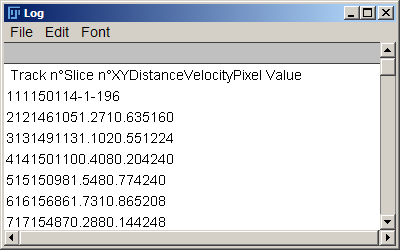
\includegraphics[scale=0.6]{fig/fig253_AllValuesinLog.png}
\caption{Manual Tracking Results in Log window}
\label{fig:manualtrackingresultsLog}
\end{center}
\end{figure}

So far so good, we succeeded in getting data out of the results table. 
Then what we need to do now is to play around with the \ilcom{str} variable, 
where all the data is now contained as a chunk. Since this chunk of data is not usable directly, 
we first split the \ilcom{str} to single lines of a string array. 
For this we use the \ilcom{split} function, the definition of which is 

\begin{indentCom}
\textbf{split(string, delimiters)}\\
Breaks a string into an array of substrings. 
Delimiters is a string containing one or more delimiter characters. 
The default delimiter set " \textbackslash{}t\textbackslash{}n\textbackslash{}r" 
(space, tab, newline, return) is used if delimiters is an empty string or split is called with only one argument. 
Returns a one element array if no delimiter is found. 
\end{indentCom}

Using this function to convert the string to a string array and adding two more lines to check the content of the array, 
the code now looks like this:\\
\begin{lstlisting}[numbers=none, morekeywords={*, split}]
str = getInfo("window.contents");
//print(str);
strA = split(str, "\n");
print(strA[0]);
print(strA[1]);
\end{lstlisting}
We use the delimiter \ilcom{\textbackslash{}n} which means "new line", a hidden character in \ilcom{str} 
that feeds a new line to form a table. When we run the above code we will see two lines of data shown in the log window (Fig. \ref{fig:splittedLine}).
%figure 
\begin{figure}[htbp]
\begin{center}
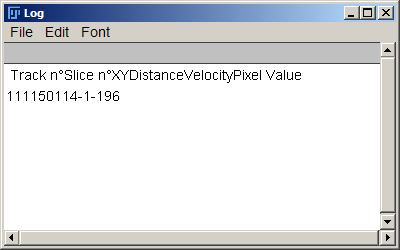
\includegraphics[scale=0.6]{fig/fig253_ZeroAndfirstlineValues.png}
\caption{Two Lines from data in the Log window}
\label{fig:splittedLine}
\end{center}
\end{figure}

We then still need to split each single line to individual data for each column. We modify the code as follows:
\begin{lstlisting}[numbers=none, morekeywords={*, split}]
str = getInfo("window.contents");
strA = split(str, "\n");
lineA = split(strA[1], "\t");
print(lineA[3]);
\end{lstlisting}

We use the delimiter \ilcom{\textbackslash{}t}, which means "tab", to convert a single line to an array of individual pieces of data (one element for each column). 
%figure 
\begin{figure}[htbp]
\begin{center}
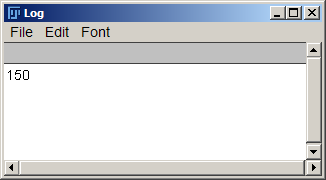
\includegraphics[scale=0.6]{fig/fig253_XfirstlineValue.png}
\caption{Elementary data in the Log window}
\label{fig:doublesplittedLine}
\end{center}
\end{figure}

The value shown in the Log window (Fig. \ref{fig:doublesplittedLine}) 
should be the same as the X value in the first row of the original table (Fig. \ref{fig:manualtrackingresults}). 

We now know how to access individual data values within \ilcom{str}, 
by first splitting it with delimiter \ilcom{\textbackslash{}n} and then by
\ilcom{\textbackslash{}t}. We can print all XY coordinates in the Log window with the following code.  

\lstinputlisting[morekeywords={*, split}]{code/code25.ijm}

If you encounter an error message with \ilcom{lineA[]} such as shown in fig.\ref{fig:fig262_ErrorMessage}, 
this is just because there is another text widow open and the \ilcom{getInfo()} function worked on 
that window rather than the results table of the Manual Tracking. To avoid such error, 
close the extra text windows and then try running the macro again. 
%figure  
\begin{figure}[htbp]
\begin{center}
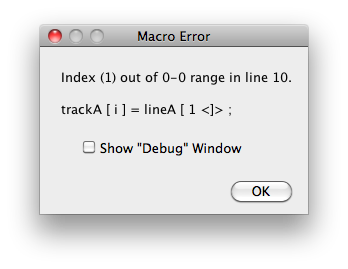
\includegraphics[scale=0.6]{fig/fig262_PossibleErrorMessage.png}
\caption{Possible Error Message with Code25 and Code25.5}
\label{fig:fig262_ErrorMessage}
\end{center}
\end{figure}

From line 4 to 7, new arrays are generated to store data from four columns in the for-loop from line 8 to 14. 

%figure  
\begin{figure}[htbp]
\begin{center}
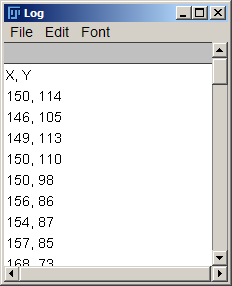
\includegraphics[scale=0.6]{fig/fig253_CoordinatesPrintedOut.png}
\caption{Elementary data in the Log window}
\label{fig:fig253_CoordinatesPrintedOut}
\end{center}
\end{figure}

Check the log window (Fig. \ref{fig:fig253_CoordinatesPrintedOut}), 
compare the output with the manual tracker results table, and if you are confident that you are accessing the right data in the table, 
you could then use the XY coordinates to place a circular ROI, 
measure the average intensity in that area and list them in the ImageJ Results window.

\lstinputlisting[morekeywords={*, split}]{code/code25_5.ijm}

Running this code, you should see a Results window that looks like figure 
\ref{fig:fig262_ManualTrackIntfinalResults}, tracking data plus measured intensity is shown in 
the column titled "RoiInt". The way the oval ROI is used to measure the mean intensity is similar to what 
we have coded in the previous subsection. A difference is that this time, we use arrays that store data 
extracted by splitting the chunk of string data. 

%figure  This should be replaced with results window!!!
\begin{figure}[htbp]
\begin{center}
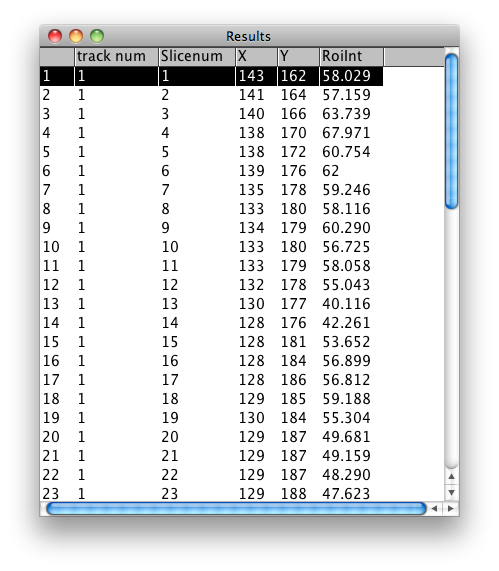
\includegraphics[scale=0.5]{fig/fig262_ManualTrackIntensityFinalResults.png}
\caption{ Manual Tracker Results in IJ Results table\\ now with measured intensity column RoiInt}
\label{fig:fig262_ManualTrackIntfinalResults}
\end{center}
\end{figure}

We then successfully measured the intensity dynamics of moving object again.  

\newpage
\subsection{Accessing Data File: Simple Case}
In this section and in the next section, 
we study how to access data in saved file for secondary measurements. 

Two cases we studied so far were both accessing data listed in a table that is already loaded in ImageJ 
(data is already an instance of ImageJ). What if we want to use data that is saved as a file? For example, 
we want to use results of Manual Tracking (previous section) that was saved as an .xls file and 
you want to use its data for secondary measurement. More generally, you did particle tracking using different software 
such as Imaris Track, and you want to use  coordinate data from that analysis for intensity measurement to be done in ImageJ. 
In such cases, we should access tabulated data in file accessing from ImageJ. 

In this section, we try accessing data saved by Manual Tracking. 
Loading data file could be done by a small modification 
of the code we studied in the previous section. Instead of the function 
\ilcom{getInfo("window.content")} in line 3 of code 25.5, we use \ilcom{FileOpenAsString(path)} to retrieve 
file content into a string variable.  By leaving the argument \ilcom{path} blank (""), user will be asked for choosing a file. 
Since this is a simple one-line replacement of line 3 of code 25.5, below is the new code but only showing its first 10 lines.  

\lstinputlisting[linerange={1-10}, morekeywords={*, File, openAsString}]{code/code26.ijm}

To run this macro, be sure that you have your stack already opened, as it is required for measuring intensity. 

\subsection{Accessing Data File: Complex Case}

We now try making use of data file with more complex format. 
In the case we studied with Manual Tracking plugin in the previous section, data format was pretty straight forward 
so we did not have to do much work for dealing with the data format. 
In general, things are not so simple and one must figure out some way to decode the format for using it in secondary measurement. 

Automatic tracking plugin "ParticelTracker" allows you to save trajectory data by "Save Full Report" 
button in the results interface (see Fig. \ref{fig:particletrackingresults}). 
We try to access this data. 
\footnote{ This technique is especially important if you want to do automated particle tracking of many data. 
A new feature in ParticleTracker plugin released in Nov. 2010 is that when ParticleTracker is called from macro, 
it automatically saves data in folder where the image file is located. We then are able to process many files using macro, 
even recursively, and get tracking data automatically. For this reason technique for accessing ParticleTracker data file is valuable.}

First, you must prepare the data file. 

\begin{indentexercise}{1}
\item Open sample image stack \textbf{TransportOfEndosomalVirus.tif}. 
Then do \ijmenu{[Plugins > Particle Detextor \& Tracker> Particle Tracker]}. 
An interface appears, so fill in the parameters as follows:
\begin{itemize}
\item radius: 3
\item cutoff: 0
\item percentile: 0.3
\item link range: 1
\item distance: 20
\end{itemize}
\item Click "Save Full Report" and save the data file in the folder where sample image stack 
"\textbf{TransportOfEndosomalVirus.tif}" is. 
Saving dialog will come up with a proposal of file name to be "Traj\_<filename>.txt" 
so do not change that and simply click Save (this file name will be important). 
Close the Results interface. Do not close the image stack \textbf{TransportOfEndosomalVirus.tif}, 
as we will use it still in the following.
\end{indentexercise}

Now you are ready with data, so we try loading data into ImageJ/Fiji. Run the following code. 

\lstinputlisting[morekeywords={*, substring, lengthOf,File, exists, openAsString}]{code/code27_PTfileaccess.ijm}

You now have all the values in the log window, that should look like fig. \ref{fig:fig264_PTdatainLogWin}. 

%figure  
\begin{figure}[htbp]
\begin{center}
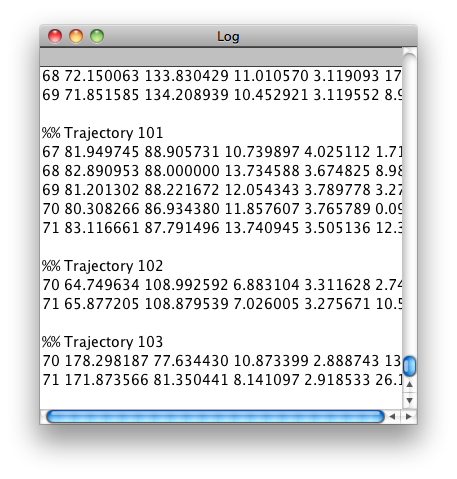
\includegraphics[scale=0.5]{fig/fig264_PTdataLoadedtoLog.png}
\caption{ ParticleTracker data loaded to Log Window}
\label{fig:fig264_PTdatainLogWin}
\end{center}
\end{figure}

Before getting into data file structure, let's look at what we have done in the code above. 
You might then study about how to deal with string, extracting parts of it. 
\begin{itemize}
\item Line 2: \ilcom{getDirectory} function with option \ilcom{("image")} 
will return a path of the last-opened image location. 
This will be where the file "\textbf{TransportOfEndosomalVirus.tif}", inside the sample image folder. 
\item Line 3: Filename of the image  "\textbf{TransportOfEndosomalVirus.tif}" is acquired. 
\item Line 4: Generating the file name of the data file. "Traj\_" is the prefix that was automatically added to 
the data file name. Function \ilcom{substring} extracts part of the string variable, and in our case, 
we try to get the image file name without ".tif". Definition of \ilcom{substring} function is as follows.

\begin{indentCom}
\textbf{substring(string, index1, index2)}\\
Returns a new string that is a substring of string. The substring begins at index1 and extends to the character at index2 - 1. 
See also: indexOf, startsWith, endsWith, replace.
\end{indentCom}

index1 should be 0, as we want from the beginning of the file name, and index2 should be 4 strings before the 
last string so we need the total length of the string. For this we use \ilcom{lengthOf} function. 
\begin{indentCom}
\textbf{lengthOf(str)}\\
Returns the length of a string or array.
\end{indentCom}
In this way, we construct the file name we want to access 
(the name of which originally is automatically generated when saving the data in Particle Tracker interface) 
the file further setting the full path to the file in line 5. 
\item Line 8: This line checks if the file full path generated above is valid. 
\ilcom{File.exists(full-path-to-file)} returns false if there is no such file. In that case, we should not proceed more so macro terminates at line 8. 
\item Line 11: If everything is ok, then the file is opened as a string, 
and the string will be printed in Log window by line 12. 
\end{itemize}

ParticleTracker data file consists of three parts. 
\begin{enumerate}
\item Header: contains information on the condition of tracking. 
\item Detected Particles: Detected particles in each frame is listed.
\item Trajectories: Trajectories are listed, one by one. 
\end{enumerate}
Since we need to access trajectory information, we need to go through the data string to reach the third part of the data structure. 
To do so we split the file by lines (\textbackslash{}n), then loop through the array to find the position where the trajectory information is contained. 

We examine the data file in detail, to see what could be the marker for the starting and end point of each trajectory. 
Here is a part of data, that is a directly copy and pasted below. 
\begin{lstlisting}[numbers=none]
24 154.894485 137.063614 7.338140 3.316167 15.683273
25 154.217377 138.368927 7.087145 3.417947 0.188002

%% Trajectory 37
15 22.111439 204.511826 9.726052 3.180977 28.252821
16 8.837964 209.618210 13.082743 3.273177 29.163294
17 0.432002 208.377045 3.574241 1.552869 0.000000
18 2.150804 209.609573 11.131773 2.939974 13.455443
19 10.542578 206.151169 14.173851 3.202391 14.258223
20 9.727753 206.960999 14.360144 3.250930 6.493425
21 15.708366 207.058640 14.943080 3.121640 0.053831
22 26.715679 208.680145 14.648912 3.091611 1.570746
23 29.143650 208.706314 13.616717 2.975144 21.279413
24 28.148304 202.200867 12.116886 2.862307 6.292521

%% Trajectory 38
15 142.326370 81.088326 5.813046 2.967546 13.995440
\end{lstlisting}
Single trajectory data start with a line with "\%\%Trajectory " plus numbering, and ends with a blank space. 
We use these information as markers for determining the location of trajectory data within file. Each line of data consists of 6 numbers: 
\begin{enumerate} 
\item Frame number
\item Y coordinate
\item X coordinate
\item image moment m0
\item image moment m2
\item Non-Particle Discrimination Criteria
\end{enumerate}
These values are separated by space. So splitting single line to an array of elementary data needs to be done by \ilcom{split(line, " ")}.

Here is a macro, that uses \ilcom{File.openAsString("")} to load the file and then loads the trajectory information 
into Results table with the strategy explained above. 

\lstinputlisting[morekeywords={*, }]{code/code28.ijm}

In the code 28, core of the processing resides within the function \ilcom{Load2ResultsV3}. 
It takes path to the data file and file name as arguments, and first opens the file as string at line 15. 
The chunk of string is then split by lines and for-loop starts to go through the array of lines (line 19). 

In every line in the array, if the line is a starting marker "\%\% Trajectory <number>" is tested (line 22) . 
If that is the case, then do-while loop is started, that loops until all the trajectory points are read out (line 24 to 41). 
While this trajectory read out is done, counter for the for-loop \ilcom{i} 
is also incremented that when the do-while loop ends (line 25), the for-loop starts again from the 
line after the data of that trajectory. Exit from do-loop occurs when blank line is found (line 42). 

Inside the do-while loop, space character is replaced with tab delimiter (line 26 to 32). 
This is required, since ImageJ results importing only recognized tab-delimited file as a table.  

There is a small adjustment by another function \ilcom{CommaEliminator} at line 32. 
This is required for removing comma character in some cases (this happens when the data file was opened and saved in excel or so). 
You probably do not need this line and function as we are using the data file directly after saving them. I left it in the code for your future usage. 

Just to be sure with data content, line 33 and 34 double-check that the line indeed contains several data. 
Line 35 to 38 writes trajectory ID, Frame number and XY coordinates into Results window by \ilcom{setResult} function.

\begin{indentexercise}{2}
\item Finally, we can combine several macros and functions we studied so far to make a new macro 
that loads the ParticleTracker data file to Results table, and read out intensity. 
This could be done by combining following codes, with a bit of modifications with each. 
\begin{itemize}
\item code 27 (check the current image stack name and loads its track data file as string)
\item code 28 (data in string format is converted to Result table)
\item code 24.5 (measure intensity according to coordinates in Results table)
\end{itemize}
Bits and pieces are already there. Please try completing a macro that loads track data file according 
to the title of the image stack that is already opened, place them in Results table, and then measure 
the intensity in corresponding frame and position in the image stack. 
\end{indentexercise}

\newpage

\section{Using Javascript}

As you become experienced with coding in ImageJ macros, you might start to find
out that for whatever you want to do with ImageJ, 
corresponding macro function does not exist in the Build-in Macro Functions page
\footnote{ see \url{http://rsb.info.nih.gov/ij/developer/macro/functions.html}}. 
One way to supplement the missing function is to create your own user function. 
Another way is to find a function directly from ImageJ Java code and use that function in macro. 
Javascript is a convenient way to access ImageJ API (Application Programming Interface), 
and since Javascript could be called from within ImageJ macro, you could use ImageJ API in your macro code. 
This is done by the macro function shown below:
\begin{shaded}
\begin{indentCom}
\item \textbf{eval("script", javascript)}\\
Evaluates the JavaScript code contained in the string javascript.\\
\end{indentCom}
\end{shaded}

This would be the simplest way to use Javascript if you are already
comfortable with ImageJ macro language. 

\textbf{But there is more to it}. You could also run Javascript as it is in
ImageJ and Fiji. Syntax of Javascript is not same as ImageJ macro, 
but if you are used to write ImageJ macro, it should not be too difficult to learn Javascript.  
 
\dots then how could we code Javascript? 

In this section, we learn basic know-how of 
Javascript with ImageJ 
\footnote{ If you want to learn in more detail, 
you could also visit \url{http://pacific.mpi-cbg.de/wiki/index.php/Javascript_Scripting} 
for learning more about Javascript.}. Experience with 
Java programming is largely helpful but if not, there is also some way around
to learn quickly. 

When we are programming ImageJ macro, we often refer to the
web site listing ImageJ macro language functions to look for a macro function. 
In similar way, we access so called API (Application Programming Interface) 
for coding with Javascript. ImageJ API is in the following page:

\url{http://rsb.info.nih.gov/ij/developer/api/index.html}

At this moment, you might be puzzled with these pages, 
but don't worry. Major aim of this section is to learn how to use this resource 
to code your Javascript. 

OK, let's start. 

\subsection{A trial with Javascript}
%
Let us first try using Javascript (JS). 

From menu, do \ijmenu{[Plugins > Scripting > Javascript Interpreter]}. 
You will then see a new interface that looks like Fig \ref{fig:JSinterpreter}. 
This interface provides Javascripting in an interactive mode and is useful for 
a quick testing of codes. There is a input field at the bottom, where you could type in JS code. 
Then by pressing return key, the code is executed.  

\begin{figure}[htbp]
\begin{center}
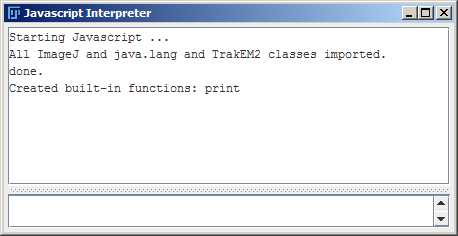
\includegraphics[width=100mm]{fig2/JSinterpreterStasrtUp.png}
\caption{Javascript interpreter on start up.}
\label{fig:JSinterpreter}
\end{center}
\end{figure} 

Type the following command and execute by return key. 
\begin{lstlisting}[numbers=none]
IJ.log("Hello JS")
\end{lstlisting}
This JS command will print "Hello JS" in the Log window of ImageJ.  

Same command could be written in the Script editor. To start up the editor, 
do \ijmenu{[File > New > Script]} (then select \ijmenu{[Language > Javascript]}). 
\begin{lstlisting}[numbers=none]
IJ.log("Hello JS");
\end{lstlisting}
This should do the same thing, but be careful! Do not forget adding semicolon
(;) at the end of the line. In case you write your code in Script Editor, you need
to explicitly mark the end of line, just like you do when you write a macro.

To run the code, \ijmenu{[Run > Run]} will execute the command (you could also
use ctrl-r or cmd-r). 

What this JS code does is the same as the Macro code below. 
\begin{lstlisting}[numbers=none]
print();
\end{lstlisting}

In the following, you could use either Javascript interpreter 
or Script editor. Just choose the one you like. If code become multiple lines, 
I recommend you to use the Script Editor\ldots and in this case, this is a
redundant warning, place a semi-colon ``;'' at the end of each line.

Now, we could try some commands that is not present in 
ImageJ macro.
 
For example, what would you do if you want to convert angle in degrees to radian? 
In macro, you could do calculation by first dividing the value by 360, 
then multiply by $2\pi$. But a function actually is already there in Java, 
so you could simply use that as well. 
\begin{lstlisting}[numbers=none]
IJ.log(java.lang.Math.toDegrees(3.1415)) 
\end{lstlisting}
Running this line should print a number close to 180. You could also do the
other way around:
 \begin{lstlisting}[numbers=none]
IJ.log(java.lang.Math.toRadians(180)) 
\end{lstlisting}
should print out 3.1415\dots.

Next, we try to retrieve a column of data from table in Results window. 
In macro, you could do this by \ilcom{getResult} function, 
with which by specifying the column label and row number you could retrieve 
a value in that cell. 

But what should we do if we want to retrieve all data in a row at once, 
not a single value in a specific column at specific row? 
If you want to do this in macro, we could write a user defined function that loops 
for all the columns and get data one-by-one. 

With Javascript, this could be done in just a single step, one command. 

\begin{indentexercise}{1}

\textbf{Preparation of Results table}

Open image by \ijmenu{[File > Open Sample > blobs (25k)]}. 

Check measurement parameters by 

\ijmenu{[Analyze > Set Measurements\dots]}

that some measurement parameters are checked. Be sure that "Limit to Threshold" is checked. 

Then Threshold the blob image by 

\ijmenu{[Image > Adjust > Threshold]}. 

Since the background of this image is bright, Dark Background' should be unchecked. 
If you see the thresholded image like fig. \ref{fig:ThresBlob},  do 

\ijmenu{[Analyze > Analyze Particles\dots]}. 

%figure
\begin{figure}[htbp]
\begin{center}
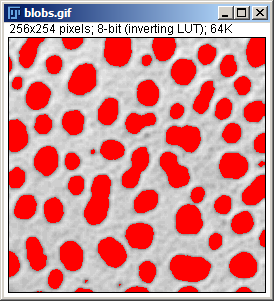
\includegraphics[height=50mm]{fig2/ThrehsoldedBlob.png}
\caption{Thresholded image of "blob"}
\label{fig:ThresBlob}
\end{center}
\end{figure} 

In the Analyze Particles dialog, just be sure that \textbf{Display Results} is checked. 
Then click OK button. When the analysis is done, you will see  64 or so particles detected 
and listed in the Results window. 

\textbf{Testing Javascript Code}

We now use the following command to extract data from single Row. In Javascript
interpreter, type the following command .

\begin{lstlisting}[numbers=none]
IJ.log(ResultsTable.getResultsTable().getRowAsString(10));
\end{lstlisting}

If you execute this, you will see that all data that is in row 11 in Results table is 
now printed in the log window. 

\dots that's the end of this exercise but don't close the Results window yet.   
\end{indentexercise}

Above is a single line pure JS code. 
We can use this code within macro by using \textbf{eval} function mentioned already. 
Here is an exercise to test the function \textbf{eval}. 

\begin{indentexercise}{2}
Test running the following code, and check that any row in the table could be extracted 
and printed in Log window. 
\begin{lstlisting}
rownum = getNumber("Row?", 0);
jscom = "IJ.log(ResultsTable.getResultsTable().getRowAsString("+rownum+"));";
eval("script", jscom);
\end{lstlisting}
\end{indentexercise}

In the second line, JS code is constructed as a single string \ilcom{jscom} 
using the variable \ilcom{rownum} from line 1. Line 3 executes this JS code using \textbf{eval}. 

So far, I have not yet explained where these commands came from. 
I will give more detailed explanation in later sections.  

\begin{indentexercise}{2}
This exercise is optional:

Try the following Javascript commands using \textbf{eval}, from within an ImageJ
macro.

\dots lists all ImageIDs. There should be at least one image opened. 
\begin{lstlisting}[numbers=none]
a = WindowManager.getIDList();
for(i in a) IJ.log(a[i]);
\end{lstlisting}

\dots zooms current image centered at top-left corner.
\begin{lstlisting}[numbers=none]
IJ.getImage().getCanvas().zoomIn(0, 0);
\end{lstlisting}

\dots print souts statistics of current image in log window.
\begin{lstlisting}[numbers=none]
eval("script", "IJ.log(IJ.getImage().getStatistics().toString());");
\end{lstlisting}

\dots print outs used memory in log window.
\begin{lstlisting}[numbers=none]
eval("script", "print(IJ.currentMemory())");
\end{lstlisting}

\dots moves current image window to top-left corner of the monitor with offset of 10 by to, 
and resizes the window. 
\begin{lstlisting}[numbers=none]
eval("script", "IJ.log(IJ.getImage().getWindow().setLocationAndSize(10, 10, 100, 100))");
\end{lstlisting}
\end{indentexercise}

In all the example codes, we placed Javascript commands in the second argument 
for the function \textit{eval}. 
You could also write a full path to a Javascript file. Here is the syntax. 
\begin{shaded}
\begin{indentCom}
\item \textbf{eval}('script', \textbf{File.openAsString}("<pathpath>/name.js")) ;
\end{indentCom}
\end{shaded}

\subsection{Using Macro Recorder and ImageJ API}
Javascript is a scripting language, so it has its own build-in functions. 
I will not explain about this since you could find many Javascript tutorials on the web. 
For example, following site is a place where I go and look for Javascript commands and usages:

\href{http://www.w3schools.com/jsref/default.asp}{Javascript Reference @ w3chools.com}

How do we find Javascript commands to interact and control ImageJ? 
The easiest way is to use the macro recorder. 
We have already learned and used macro recorder in previous chapters. 
We could used the same interface for recording JS codes. 
Recorded lines of JS codes could be copy \& pasted into Script Editor and can be directly executed. 

\begin{indentexercise}{1}
First, we should start the recorder. 
\ijmenu{[Plugins > Macros > Record\dots]}. 
Then in the recorder window at the top-left corner, 
choose Javascript as the code to be recorded (Fig. \ref{fig:MacroRecorderJS}). 

%figure
\begin{figure}[htbp]
\begin{center}
\includegraphics[width=70mm]{fig2/RecorderJS.png}
\caption{Setting Up Macro Recorder ready for Javascript}
\label{fig:MacroRecorderJS}
\end{center}
\end{figure}

Then do the following sequence of commands.
\begin{itemize}
\item \ijmenu{[File > Open Sample > Blobs]}
\item Select rectangular ROI tool and set a ROI to select 
about 1/4th of the image (can be any place within the image. This is just a test.). 
\item \ijmenu{[File > Transform > Flip Horizontally]}
\item \ijmenu{[Process > Filters > Gaussian Blurr\dots]}
\end{itemize}
After all these operations, there should be JS codes printed in the Recorder window. 
Copy them all, and paste it to Script Editor (\ilcom{[File > New > Scripts]} and then paste, 
Fig. \ref{fig:ScriptEditorRecorded}) . 
After pasting, set language to JS by (\ilcom{[Language > Javascript]} from the menu bar of script editor.  

%figure
\begin{figure}[htbp]
\begin{center}
\includegraphics[height=50mm]{fig2/JSrecordedInScriptEditor.png}
\caption{Javascript by recorder commands.}
\label{fig:ScriptEditorRecorded}
\end{center}
\end{figure}

Then do \ilcom{[Run > Run]} from the menu of script editor, the script is executed. 
You should then see a new window of "blob" with some part of image processed. 
\end{indentexercise}
If you are successful in running the code, let's see the code. Here is how the code should look like. 

%\lstinputlisting[morekeywords={*}]{code/code29.js}
\lstinputlisting{code/code29.js}

We first examine line 3 and line 4, focusing on the method \ilcom{IJ.run}  
(in the follwoing, we use word "method" instead of "command", as this is more 
conventional way of calling it in Java). This method has three arguments for it.

\ilcom{IJ.run(argument1, argument2, argument3)}

 Just by looking at each of them you could realize that the second argument 
 is a descriptive explanation of what the method does. 
 This is because these strings are exactly the phrase of the menu item you see 
 when you choose that function from ImageJ menu. 

\ilcom{IJ.run} is a method that uses second argument as a keyword 
to search for all the ImageJ menu items to find which of them is the one 
that the method intends to invoke 
\footnote{In ImageJ macro, a function similar to \ilcom{IJ.run} 
method is \ilcom{run(arg1, arg2)}.}. 
Third argument of \ilcom{IJ.run} in line 3 is an empty string, 
but in line 4, the third argument is \ilcom{sigma=2}. 
This is a value that you normally input when you select Gaussian blur 
from the menu bar for the size of blurring kernel. 

Then what is the first argument in \ilcom{IJ.run}? 
In both line 3 and 4, we have a variable \textbf{\ilcom{imp}}. 
To see what this is, we go back to line 1. 
\textbf{\ilcom{imp}} appears for the first time in the code at line 1, 
and \textbf{\ilcom{imp}} is the returned value of a method \ilcom{IJ.openImage}. 
If we think back what we were actually doing for this first line when recording, 
we accessed an item in the menu tree \ijmenu{[File > Open Sample > blobs]}. 
By choosing this item from menu, ImageJ downloads blobs.gif file from NIH web site 
and then shows it on your desktop. 
Single method that does the download action is the method \ilcom{IJ.openImage}. 
Argument for this command is the URL of the image. 

To know the definition of the method \ilcom{IJ.openImage}, 
we look up a reference called 
\href{http://rsb.info.nih.gov/ij/developer/api/index.html}{ImageJ API}
\footnote{ ImageJ API: http://rsb.info.nih.gov/ij/developer/api/index.html}. 
In this web page, there is side bar in left side, with upper part 
for a list of "All Packages" 
(These packages are same as those listed in the table shown in the top page) 
and the bottom part for "All Classes".  

%figure
\begin{figure}[htbp]
\begin{center}
\includegraphics[height=75mm]{fig2/IJAPItop.png}
\caption{ImageJ API}
\label{fig:IJAPItoppage}
\end{center}
\end{figure}


Each package contains several classes. 
We currently do not know which package does 
\ilcom{IJ.openImage} belong to, so we look for it in the bottom part "All Classes". 
There, you will find "IJ"\footnote{ Unlike ImageJ macro, Java and Javascript are case sensitive}. 
Click the link, and in the right side of the page, a page titled "Class IJ" appears 
(Fig. \ref{fig:IJAPClassIJ}). 

%figure
\begin{figure}[htbp]
\begin{center}
\includegraphics[width=75mm]{fig2/IJAPI_IJ.png}
\caption{ImageJ API Class IJ}
\label{fig:IJAPClassIJ}
\end{center}
\end{figure}

The page might look cryptic to you, if you scroll down the page, there is a table titled "Method Summary", listing all the methods that class IJ contains in alphabetical order. 
Within this list, you will find (Fig. \ref{fig:IJAPIIJopenImage})

\ilcom{openImage(java.lang.String path)} 


%figure
\begin{figure}[htbp]
\begin{center}
\includegraphics[height=75mm]{fig2/IJAPI_IJopenImage.png}
\caption{ImageJ API Class IJ, openImage method}
\label{fig:IJAPIIJopenImage}
\end{center}
\end{figure}

There are three \ilcom{openImage} methods, with difference in number and types of arguments. 
The first one is without any argument, the second one has only one argument, 
the third having two arguments. 
When openImage method is called, one of these three are called depending on the number 
and types of the argument in the call. 

\textbf{More Explanation:} So what are "Classes?" A class consists of two major components. 
One is Field and the other is Method. 
The former is like variable and the latter is similar to function in ImageJ macro 
(this is not a precise analogy, but for now let's think like that). 
Fields are values. Methods are actions. Class is a group of various field values and methods. 
By utilizing Class, we can have a single unit of assembled functions, 
which would be an advantage for letting an application to have high modularity. 
You could access (or use) fields and methods by appending them behind the name
of the class. For example. <class name>.<field name> or <class name>.<method name>(<arguments>) 
e.g. \ilcom{IJ.openImage(pathname)}.

 \textbf{A bit more on API page} At the top of the Class IJ page (Fig.\ref{fig:IJAPClassIJ}), 
 "ij" is written above the class name "Class IJ". 
 This is the name of package that is containing this class. 
 You could see all classes within the package ij (note: case sensitive), 
 click "ij" in the left top panel listing "all packages".  
 You then will see all the classes within the package ij, 
 such as compositeImage, Executor, IJ, ImageJ\dots and so on. 
 Package is used to organize classes in hierarchical tree. 
 For example, there are packages ij.plugin, ij.plugin.filter and ij.plugin.frame. 
 Likewise, package is a tree-like structure (remember how folders are organized in your laptop) 
 that organizes many classes in a structure. In Java, such tree-like structure
 is organized separated by dots (``.''). For example, see
 \href{http://rsb.info.nih.gov/ij/developer/api/ij/plugin/filter/package-summary.html}{Package
 ij.plugin.filter}. The package filter is under the plugin package, that is
 under the ij package. 
  
Go back to the API description, in the left side of the table column where 

\ilcom{openImage(java.lang.String path) } 

is listed (Fig. \ref{fig:IJAPIIJopenImage}), there is a phrase 

\ilcom{static ImagePlus} 

This tells you that if you invoke method \ilcom{openImage(java.lang.String path)} of class \ilcom{IJ}, 
a object called ImagePlus is returned (forget about the notion "static" for now). 
ImagePlus is another class, which you could also look up using the list of "All Classes".  

The class ImagePlus consists of image data and metadata fields, and methods to access these values. 
In \href{http://rsb.info.nih.gov/ij/developer/api/ij/ImagePlus.html}{ImagePlus API page}, 
you could see that many fields and methods are associated with this class. 
Note that many of field values are "protected". 

For example, \ilcom{nChannels} is one of the filed values of class ImagePlus 
but having a notion "protected" means that you cannot simply access from outside the class itself. 
Instead, there is a method named \ilcom{getNChannels()} for accessing the value 
from outside which by invoking it "Returns the number of channels" of ImagePlus object. 
\ilcom{getNChannels()} returns a value indicated as "int". 
This tells you that the type of returned object is "int", which means that returned value is a number, 
and specifically an integer, not a number with decimal points. Unlike ImageJ macro 
\textbf{object} with any type of class could be returned, not limited to number, string and array. 
This flexibility affords higher potential in modularity with Javascript compared to ImageJ macro 
and hence we call returned values as "object" not "variables". 

A draw back is that Javascript coding becomes a bit more complicated then macro
coding. One should always be careful about which class or type is returned, 
and one way to do so is to check ImageJ API every time you wonder what is the
returned value of certain method.

Let's go back to the code again. 
The method \ilcom{IJ.openImage} returns an \textbf{object "ImagePlus"}, 
so in line 1 of the recorded Javascript code, 
an instance of ImagePlus object (which actually is "blob.png" downloaded from the NIH website) 
is stored in the variable "imp". 
Then after line 1, \ilcom{imp} behaves as an ImagePlus object. 
\ilcom{imp} is repeatedly used from line 2 to 5. In line 2, an method of class ImagePlus is invoked 
in the form <class>.<method>(arguments). 
Since method name is \ilcom{setROI} we look for it in the 
\href{http://rsb.info.nih.gov/ij/developer/api/ij/ImagePlus.html}{ImaegJ API ImagePlus page}, 
and you will find the following description:

\begin{quote}
void | setRoi(int x, int y, int width, int height) \\
          Creates a rectangular selection.
\end{quote}

"void" means that this method does not return any value. 
There are four arguments and all of them are "int", integer. 
Description tells you that this methods creates an ROI in the image with position and size 
defined by arguments.  

In line 3 and 4, the first argument of \ilcom{run} method is \ilcom{imp}, 
telling the command \ilcom{IJ.run} to do the operation specified by the second argument on \ilcom{imp}. 

Note that in case of ImageJ macro, target image could only be specified by 
activating the window using \ilcom{selectImage(imageID)}. 
In Javascript, selection of image could be more explicit by the direct use of ImagePlus object.  

Down to line 4, blob image actually is not shown on the desktop. 
ImagePlus object of "blobs.tif" is in the memory, but still is not displayed. To
show it on the desktop, we do line 5.

\begin{quote}
\ilcom{imp.show();}
\end{quote}

\ilcom{show()} is a method of ImagePlus class to show the actual image of ImagePlus object. 

%In case of Macro, we could execute that as a single line. 
% So how about doing the same? 
% Create a new script tab by \ijmenu{[File > New]} 
% from the script editor menu. 
% Then copy line 4 and paste that single line in the new script.

\textbf{Grabbing Image}
What if you want to capture already opened Image as a ImagePlus object? 
This could be done by using a method in Class IJ called \ilcom{getImage()}. 
You could replace the first line in the code we just studied with \ilcom{IJ.getImage()} 
to grab currently active image rather than downloading and opening an image file. 

\begin{indentexercise}{1}
Modify code 29 so that this JS code grabs currently active image and do the same processing. 
\end{indentexercise}

\begin{indentexercise}{2}
We study the nature of ImagePlus object in this exercise. We start with a simple
code to open an image, then add more lines to see how ImagePlus instance
behaves. Type in the code below to start up. 

\lstinputlisting{code/code30_1.js}

As we have done already, this will show a blobs.gif image on your desktop. We
can have another window with blobs.gif by adding two more lines. 

\lstinputlisting{code/code30_2.js}

We now have two instances of ImagePlus object. These are independent. 
Whatever you do to imp, that does not affect imp2. We could do a small trick
that two windows could share the the same image, that the same image appearing
in two windows. Close two windows of blobs, and then modify the code as shown
below.

\lstinputlisting{code/code30_3.js}

Run this code, and you would see two windows with same image, which seemingly
are same as before. 

Take one image and try to select some region using a ROI tool,
and from Fiji menu do \textit{[Edit > delete]}. Then the selected region blacks
out or whites out. Click another blobs window. Then you would see that the
second window, which you did not process anything, also is processed. 

This is because both windows are sharing the same image, shown in two windows.
In other way of saying, there is a single instance of image with two ImagePlus
instances. In the modified code, an extra line is added in line 3, and line 4 is
changed. Line 3 is generating a pointer (ip) to the image that is contained in
the ImagePlus instance \textit{imp}. In the 4th line, a new instance of
ImagePlus is created using what we call ``constructor'' (see ImagePlus API for
a list of constructor), using the ip that is actually associated with the
preexisting ImagePlus \textit{imp}. Finally, the 5th line shows the second
window \textit{imp2}, the image content of which is shared with \textit{imp}. 
 
\end{indentexercise}

\textbf{Summary}
\begin{itemize}
\item Object should be either created (initialized, of "Constructed") or Grabbed. 
\begin{itemize}
\item \ilcom{IJ.openImage(path)} creates and image object from file.
\item \ilcom{IJ.getImage()} grabs already existing object. 
\end{itemize}
\item Object is constructed taking a class as template. A class has field values and methods. 
Hence, object has those values and classes. 
\begin{itemize}
\item Field values are in most cases accessed via methods.
\item Once an object is constructed, its public method could be used
\end{itemize}
\item Exception: So called "static" methods could be accessed any time. 
\begin{itemize}
\item Most of methods in Class IJ are static, so you do not need to construct
it.
\end{itemize}
\end{itemize}

\subsection{Example Codes}

In this section, I will just show Javascript example using ImageJ
API\footnote{Javascript cookbook is also available in the CMCI website for
various coding examples. Visit
\url{http://cmci.embl.de/documents/110822jsip_cooking/javascript_imagej_cookbook}}.

Curve Fitting example. 
\lstinputlisting{code/codeCurveFitting.js}


\subsection{Using none-ImageJ libraries in Fiji}

Besides access to ImageJ API, power of Javascript is in importing external packages 
written in Java to use their functions.

In Fiji, many java libraries (packages) are included besides ImageJ itself. 
You could see them listed in \href{http://fiji.sc/javadoc/}{Fiji API}. 
Here are some picks among them, which might be interesting to use for math and statistics 
in Javascript\footnote{ If you want to use these packages in ImageJ, 
you could download the package from its website and configure ImageJ 
to include that package on start up.}. In the next section, 
we will study several examples to know how to import these libraries in Javascript. 

\href{http://math.nist.gov/javanumerics/jama/}{Java Matrix Package (JAMA)}
\begin{shaded}
\begin{quote}
 JAMA is comprised of six Java classes: Matrix, CholeskyDecomposition, 
 LUDecomposition, QRDecomposition, SingularValueDecomposition and EigenvalueDecomposition.

The Matrix class provides the fundamental operations of numerical linear algebra. 
Various constructors create Matrices from two dimensional arrays of double precision 
floating point numbers.  Various gets and sets provide access to submatrices and matrix elements. 
The basic arithmetic operations include matrix addition and multiplication, 
matrix norms and selected element-by-element array operations.  
A convenient matrix print method is also included.

Five fundamental matrix decompositions, which consist of pairs or triples of matrices, 
permutation vectors, and the like, produce results in five decomposition classes.  
These decompositions are accessed by the Matrix class to compute solutions of simultaneous linear equations, 
determinants, inverses and other matrix functions.  The five decompositions are
\begin{itemize}
\item Cholesky Decomposition of symmetric, positive definite matrices
\item LU Decomposition (Gaussian elimination) of rectangular matrices
\item QR Decomposition of rectangular matrices
\item Eigenvalue Decomposition of both symmetric and nonsymmetric square matrices
\item Singular Value Decomposition of rectangular matrices
\end{itemize}
\end{quote}
\end{shaded}

\href{http://commons.apache.org/math/}{Apache Commons Math Package}
\begin{shaded}
\begin{quote}
Commons Math is divided into fourteen subpackages, based on functionality provided.
\begin{itemize}
\item org.apache.commons.math.stat - statistics, statistical tests
\item org.apache.commons.math.analysis - root finding, integration,
interpolation, polynomials
\item org.apache.commons.math.random - random numbers, strings and data generation
\item org.apache.commons.math.special - special functions (Gamma, Beta)
\item org.apache.commons.math.linear - matrices, solving linear systems
\item org.apache.commons.math.util - common math/stat functions extending java.lang.Math
\item org.apache.commons.math.complex - complex numbers
\item org.apache.commons.math.distribution - probability distributions
\item org.apache.commons.math.fraction - rational numbers
\item org.apache.commons.math.transform - transform methods (Fast Fourier)
\item org.apache.commons.math.geometry - 3D geometry (vectors and rotations)
\item org.apache.commons.math.optimization - function maximization or minimization
\item org.apache.commons.math.ode - Ordinary Differential Equations integration
\item org.apache.commons.math.genetics - Genetic Algorithms
\end{itemize}
\end{quote}
\end{shaded}

\href{http://xmlgraphics.apache.org/batik/}{Batic SVG Tool kit}
\begin{shaded}
\begin{quote}
Batik is a Java-based toolkit for applications or applets that want to use images 
in the Scalable Vector Graphics (SVG) format for various purposes, 
such as display, generation or manipulation.

The project's ambition is to give developers a set of core modules 
that can be used together or individually to support specific SVG solutions. 
Examples of modules are the SVG Parser, the SVG Generator and the SVG DOM. 
Another ambition for the Batik project is to make it highly extensible—for example, 
Batik allows the developer to handle custom SVG elements. 
Even though the goal of the project is to provide a set of core modules, one of the 
deliverables is a full fledged SVG browser implementation which validates the various modules 
and their inter-operability.
\end{quote}
\end{shaded}

\href{http://spaceroots.org/software/mantissa/index.html}
{Mantissa (Mathematical Algorithms for Numerical Tasks In Space System Applications)}
\begin{shaded}
\begin{quote}
Mantissa is a collection of various mathematical tools aimed towards for simulation. 
It is not a complete mathematical library like GSL, NAG or IMSL, but it contains various 
algorithms useful for dynamics simulation and 3D geometry computation.
\end{quote}
\end{shaded}

\href{http://www.cs.waikato.ac.nz/ml/weka/}{Weka}
\begin{shaded}
\begin{quote}
Weka is a collection of machine learning algorithms for data mining tasks. 
The algorithms can either be applied directly to a dataset or called from your own Java code. 
Weka contains tools for data pre-processing, classification, regression, 
clustering, association rules, and visualization. 
It is also well-suited for developing new machine learning schemes.
\end{quote}
\end{shaded}

Some other packages\dots

\begin{itemize}
\item \href{http://www.imagescience.org/meijering/software/}{ImageScience} - 
Implemented as plugins for filtering but valuable for use as a library. 
\item \href{http://www.f4.htw-berlin.de/~barthel/ImageJ/ImageJ3D/ImageJ3D.html}
{ImageJ3D - JRenderer3D} -3D renderer. 
\item kfschmidt.*  - Numerical analysis tools: Simplex, GLM analyzer, Matrix
calculations
\item math3D -Matrix calculation, 3D tools.  
\end{itemize}

\subsection{Example Use of Library}
Following will be some examples of using Apache Commons Math library. 
\subsubsection{Descriptive statistics}

\lstinputlisting{code/code32.js}

When you use a package, you should first import it. 
The first line is doing this by using a method \ilcom{importPackage}. 
One could also import a single class, using \ilcom{importClass} method. 
In line 4, a new object of Class DescriptiveStatistics is created. Line 5 and 6 stores data in this object, 
and calculates statistics in line 9, 10 and 11.

\subsubsection{Solving Linear System}
% http://commons.apache.org/math/userguide/linear.html
We could solve linear equation system below, in the form AX = B, by LU decomposition. 
\[
2x + 3y - 2z = 1
\]
\[
-x + 7y + 6x = -2
\]
\[
4x - 3y - 5z = 1         
\]

\lstinputlisting{code/code33.js}

\newpage

\section{Actual Macro programming}
The biggest tip for Macro coding: Don't try to code everything from scratch. 
Refer to the downloadable macros linked in the ImageJ web site 
\footnote{ see \url{http://rsb.info.nih.gov/ij/macros/}}, 
and there should be something you could copy some parts to full fill the task you want to achieve.\\

\begin{indentexercise}{1}
Think about your daily work with image processing / analysis, and design a macro that helps your task. 
\item 1. Present your idea. Similar macro might already exists, which could be modified for your task.  
\item 2. Write the macro after discussion with your instructor. 
\item 3. Debug the macro. If you could not finish, do it as homework. 
Turn it in, regardless of whether its working or not. 
\end{indentexercise}

\newpage

\section{Homework!}

\subsection{Homework for basics} 

\subsubsection{Assignment 1}
Change code 12.75 so that 
\begin{itemize}
\item Does not use "\&\&"(AND) 
\item Instead, uses "||" (OR). 
\end{itemize}

Comment: This is also a test if you can think things logically\ldots Thanks to Prof. Boole. 

\subsubsection{Assignment 2}

Write a macro that draws gird (lattice) in a image (see example, attached).
If you have time, modify the macro so that the macro plots diagonal lattice.
Steps should be something like:
\begin{enumerate}
\item creat a new image
\item loop in x direction and draw vertical line
\dots for this, use command \ilcom{drawLine(x1, y1, x2, y2)}
\dots see
\url{http://rsb.info.nih.gov/ij/developer/macro/functions.html#drawLine}
\item loop in y direction and draw horizontal line
\end{enumerate}


Hints: if you want to draw white lines on black image
 \begin{itemize}
\item you need to select black background when you make a new image
\item you need to set the drawing color using \ilcom{setColor()}
\item see
\url{http://rsb.info.nih.gov/ij/developer/macro/functions.html#setColor}
\end{itemize}
%composing grids
\begin{figure}[htbp]
\begin{center}
\includegraphics[scale=0.6]{fig/grid.png}
\caption{Composing grid image}
\label{fig_homeworkGrid}
\end{center}
\end{figure}

%composing diagonalgrids
\begin{figure}[htbp]
\begin{center}
\includegraphics[scale=0.6]{fig/gridDiagonal.png}
\caption{Composing grid image}
\label{fig_homeworkGridDiagonal}
\end{center}
\end{figure}

\subsubsection{Assignment 3}  
Write a macro that deletes every second frame (even-numbered frames) in a stack. 

Hint: use \ilcom{run("Delete Slice");} to delete a single slice. 

Comment: it might be tricky.

\subsubsection{Assignment 4} 
Write a time stamping macro for t-stacks. You should implement following functions. 
\begin{itemize}
\item User inputs the time resolution of the recording (how many seconds per frame).
\item The time point of each frame appears at the top-left corner of each frame.  
\item If possible, time should be in the following format: \\
mm:ss \\
(two-digits minutes and two digits seconds)
\end{itemize}
Hint: Use following: for-statement, 
\ilcom{nSlices, setSlice, getNumber,\\ setForegroundcolor, setBackgroundColor,
drawString, IJ.pad}. (refer to the Build-in Macro Function page in ImageJ web
site!)

\subsubsection{Assignment 5} 
Modify code 14 so that the macro does not use "while" loop. For example with the following way. 
\begin{itemize}
\item Macro measures the integrated density of all area in the first frame ( = ref\_int).
\item In the next frame, full integrated intensity is measured again (temp\_int).
\item Decrease the lower for the thresholding by temp\_int/ref\_int.
 \end{itemize}

\subsection{Homework for a bit advanced}

\subsubsection{Assignment 6}
Write an elementary calculator macro with single dialog box that does:
\begin{itemize}
\item user input two numbers
\item user selects either one of addition, subtraction, multiplication or division. 
\item answer appears in the Log window. 
 \end{itemize}
Hint: use \ilcom{Dialog.addChoice Dialog.getChoice} command.   

\subsubsection{Assignment 7}
Write a macro that does pseudo high-pass filtering by Gaussian blurred image
(duplicate an image, do Gaussian blurring with a large kernel to create
background and subtract it from the original). If you could successfully write a
macro, then convert it to a function and use it from a macro.
Hint: use \ilcom{getImageID(), selectImage(id)} command.   

\section{Aim: Why do we write ImageJ macro?}
  %\section{Aim: Why do we write ImageJ macro?}

The aim of this small chapter is to teach the basics of how to automate image processing and analysis using ImageJ macro language. Why do we write ImageJ macro? We write macros to decrease our workloads in image processing: less clicking and less repetitive procedures. 


\section{Introduction}
  %%% Introduction for macro programming tutorial
%%% Kota Miura (miura@embl.de)

% \section{Introduction}

\subsection{ImageJ macro makes your life easier}

To customize functions in ImageJ, a typical way is to write a Java plugin that directly accesses the application interface of ImageJ. 
This is a powerful method for customizing your own tool but in many cases is a bit too much for small tasks we often encounter in biological research projects. Compared to the Java programming, ImageJ macro is much easier for quickly solving problems.

A typical usage is to automate repetitive tasks with hundreds of times of mouse clicking. Clicking ranges from menu selections to inspection of single pixel value. By writing a macro, we could save such exhausting job to a single execution of a macro file, which is a text file with a sequence of image processing commands. As ImageJ macro functions are directly mirroring the GUI menu items, one could intuitively learn how to write one's own macro even without much experiences in programming.

Another important aspect of writing a macro is its role as a documentation: as the processing becomes complex, we easily forget the steps and details of the procedures and the values of parameters that were used for that task. Even if your job is not a repetitive one, a macro written for a task becomes a valuable record of what was done to the image, and ensures the \textbf{reproducibility} of your image analysis.  

\subsection{Other ways to Customize ImageJ}

This and the next section explain the general capability of extending ImageJ by programming. If you are not interested in general aspects, you could skip these sections.  

ImageJ could be extended by writing a Java plugin. Though you need to know or learn the Java programming,  this capability affords almost infinite possibilities;  you could write any kind of processing / analysis functions you could imagine. Compared to the plugin development by Java, ImageJ Macro language is much easier and lighter but has some limitations. It might be worth mentioning here what would be the limitations. 

\begin{enumerate}
\item If you need to process large images or stacks with many steps, 
you might recognize that it is slow. Some benchmarks indicate that a plugin would be about 40 times faster than a macro. 

\item Macro cannot be used as a library
  \footnote{It is possible to write a macro in a library fashion using the function \ilcom{eval} and use it from another macro, 
but this is not as robust and as clear as it is in Java, which is a language designed to be so.}. 
In Java, once a class is written, this could be used later again for another class. 

\item Macro is not efficient in implementing real-time interactive input 
during when the macro function is executed; 
\textit{e.g.} If you want to design a program that requires real-time user input 
to select a ROI interactively.  
Macro could only do such interactive tasks by closely related macro set with each macro doing each step of interaction. 

\item Macro is tightly coupled to GUI (Image Window), so that when you want to process images without showing them on desktop, macros are not really an optimal solution.
\end{enumerate}

If you become unsatisfied with these limitations, 
learning more complicated but more flexible Java plugin development is recommended. 


\subsection{Comparison with Other scripting languages}

Besides ImageJ macro, there are several scripting languages that
could be used for programming with ImageJ. The bare ImageJ supports Javascript (Rhino). Recent versions of ImageJ (> 1.47m,  since 6 March 2013), Jython became included in the menu as well. 
In the Fiji distribution, you could use the following languages off the shelf
\footnote{As of June, 2015}
:

\begin{itemize}
 \item Javascript
 \item BeanShell
 \item Jython (Java implemented Python)
 \item JRuby (Java implemented Ruby)
 \item Clojure
 \item Groovy
 \end{itemize}

If you set up an environment by yourself, other languages such as Scala can be used. 
Compared to the ImageJ macro language, all these languages are more general scripting languages. 

There are pros and cons. Pros of using the ImageJ Macro compared to these scripting languages are: 
\begin{itemize}
\item Easy to learn. 
ImageJ macro build-in functions are mirrors of ImageJ menu, so scripting is intuitive if you know ImageJ already. 
Macro recorder is a handy tool for finding out the macro function you need. 

\item A significant hurdle for coding with general scripting languages is that one must know the 
\textbf{ImageJ Java API} well, meaning that you basically have to know 
fundamentals of Java programming language for using these scripting languages. 

\item You could have multiple macros in one file (called 'Macro-set"). 
This is useful for packaging complex processing tasks.

\end{itemize}

Thus, ImageJ macro language is the easiest way to access the scripting
capability of ImageJ.

There are several disadvantages of ImageJ macro compared to other
scripting languages. First is its generality. Since others are based on major scripting languages, you do not need to learn a lot if you know one of them already. For example, if you know Python already, 
it should be easy for you to start writing codes in Jython (note: but you also need to know about Java). 

The second disadvantage of ImageJ macro is its extendability.
Codes you wrote could only be recycled by copying and pasting
\footnote{One could also use getArgument() and File related functions to pass
arguments from a macro file to the other, but ImageJ macro is not designed to
construct a library of functions.}.
With other scripting languages, once you write a code, it could be used from other programs
\footnote{ Calling other Javascript file from another Javascript file had been difficult but became easily possible in the Fiji distribution from March 2012.}.

Lastly, although ImageJ Macro processes with a speed comparable to
Javascript and Jython, it is slow compared to Clojure and Scala. 

\subsection{How to learn Macro programming}

In this course, you will encounter many example codes. 
You will write example codes using your own computer and run those macros. 
Modifying these examples by yourself is an important learning process as in most
cases, that is the way to acquire programming literacy. There are many excellent macro codes you could find in Internet, which could be used as starting points for writing your code\footnote{200+ macros are available in ImageJ web site. 
\href{http://rsb.info.nih.gov/ij/macros/}{http://rsb.info.nih.gov/ij/macros/}}.

\subsection{Summary}
ImageJ Macro radically decreases your work load and is a practical way to keep your image analysis workflow in text file. Less workload provides more time for us to analyze details of image data. 
The potential of macro is similar to other scripting languages and Java Plugins, all adding capability to customize your image analysis. For coding interactive procedures PlugIn works better than macro. Macro cannot be used as a library.  
Image processing by macro is slower than that by Java written plugins. 

\section{Basics}
\label{sec:ImageJMacroBasics}

	\subsection{``Hello World!''}
We first try writing a simple macro that prints ''Hello World!'' in the log window of ImageJ. 

To open the macro editor, select \ijmenu{[PlugIns -> New -> Macro]} from the menu.  
This will create a new window where you can write macro (we call this ''macro
editor'', fig\ref{fig_MacroEditor}).

\begin{indentFiji}
In Fiji you could use more advanced interface called ''script editor'' 
by \ijmenu{[File -> New -> Script]}. It should look like \ref{fig_ScriptEditor}.
In the script editor, you already see a blank text field where you could write a macro. 
From script editor's own menu, select \ijmenu{[Language -> IJ1 Macro]}. 
By sepcifying the language, syntax highlighter turns on to do automatic coloring of ImageJ functions.\footnote{The macro editor (also the Fiji script editor) has simple debugger function. Debugger assists you to correct mistakes in the code. 
This is convenient when the code becomes long. 
Macro can be written in any text editor such as "Notepad" in Windows but of course 
there is no debugger function available in this case.}.  
\end{indentFiji}

Later when you want to start writing another new macro, just generate a new tab by \ijmenu{[File > New]} and then select \ijmenu{[Language -> ImageJ Macro]} again.

Then write your first macro as shown below. In the second line DON'T forget to
indent the line using tab or spaces\footnote{In ImageJ macro, indenting is not a required
syntax for writing macros but doing this will be very very helpful afterward. You
will understand it as the macro you write becomes longer}. Omit the line
numbers! These numbers were added just for explanation.

%Code 1
%\begin{lstlisting}
%macro "print_out" {
%	print("Hello World!");
%}
%\end{lstlisting}
\lstinputlisting{code/code01.ijm}
%\lstinputlisting[language=Java]{code/code01.ijm}


\begin{figure}[htbp]
\begin{center}
\includegraphics[scale=0.6]{fig/editor_helloworld_IJ.png}
\caption{Macro Editor of ImageJ} \label{fig_MacroEditor}
\end{center}
\end{figure}

\begin{figure}[hbtp]
\begin{center}
\includegraphics[scale=1.0]{fig/editor_helloworld_singleline.png}
\caption{Script Editor of the Fiji distribution} \label{fig_ScriptEditor}
\end{center}
\end{figure}

From the macro editor menu, running the code by \ijmenu{[Macros->
Run Macro]}\footnote{"Macros" in the menu appears only when the macro editing
window is active}. You could also run the code by shortcut keys (Windows:
ctrl-r, OSX command-r) as well. 
 
\begin{indentFiji}
Fiji:  Use \ijmenu{[Run -> Run]} from the script editor menu. Shortcut keys are
same as in ImageJ. You could also use ``run'' button in the script editor. 
\end{indentFiji}
This will create a new window "Log". Within the log window, "Hello World" will
be printed.

\begin{figure}[hbtp]
\begin{center}
\includegraphics[scale=1.0]{fig/helloworld_logwindow.png}
\caption{Hello World Output} \label{fig_HelloWorldLog}
\end{center}
\end{figure}

Explanation for the Code 1:\\
\begin{itemize}
\item line 1: You are declaring that a macro code starts and the code is contained between 
curly braces \{\}. "print\_out" will be the name of macro. 

\item line2: print() function orders ImageJ to print out the content within the parenthesis 
in the "Log" window. The text to be printed must be contained within the double quotes (""). 
The best reference for ImageJ macro functions is in the ImageJ web site
\footnote{\url{http://rsbweb.nih.gov/ij/developer/macro/functions.html}}. 
For example, you could find definition of print("") function on the web site as quoted below:\\
%\item
\begin{indentCom}
%\begin{minipage}[c][18em][c]{0.85\textwidth}
\fbox{
\parbox[b][20em][c]{0.80\textwidth}{
\textbf{print(string)}\\
Outputs a string to the "Log" window. Numeric arguments are automatically converted to strings. 
The print() function accepts multiple arguments. For example, you can use print(x,y,width, height) 
instead of print(x+" "+y+" "+width+" "+height). 
If the first argument is a file handle returned by File.open(path), 
then the second is saved in the referred file (see SaveTextFileDemo).

Numeric expressions are automatically converted to strings using four decimal places, 
or use the \ilcom{d2s} function to specify the decimal places. 
For example, print(2/3) outputs "0.6667" but print(d2s(2/3,1)) outputs "0.7".
}
}
\end{indentCom}

\item line 3: a brace tells ImageJ that the code "print\_out" finishes at this line.  
\end{itemize}
So that was the very basic of how you use a macro. To integrate the macro into the ImageJ Menu bar, 
the macro must be "installed". To do so, in the editor menu, \ijmenu{[Macros -> Install Macros]} 
\begin{indentFiji}
Fiji: [Run -> Install Macro]).
\end{indentFiji}
Check IJ menu \ijmenu{[Macros -> ]} to see that the macro is now in the menu.\\


\begin{figure}[htbp]
\begin{center}
\includegraphics[scale=0.6]{fig/firstMacroInMenu.png}
\caption{Macro Now in ImageJ menu} \label{fig_MacroInMenu}
\end{center}
\end{figure}

Macro can be saved as a file and can be directly installed also. 
In the editor, do \ijmenu{[File -> Save]}. Saving dialogue window appears, 
and just save the file wherever you can remember afterwards . 
To install the macro, do \ijmenu{[PlugIns -> Macro -> Install\ldots]} 
Select the macro file you want to install.\\

%\begin{indentexercise}{1cm}
\begin{indentexercise}{1}
\item Add another line \texttt{"print("\textbackslash{}\textbackslash{}Clear");"} 
after the second line (below, code 1.5. don't forget the semi-colon at the end!). 
\item \lstinputlisting{code/code01_5.ijm}
Then test also another macro when you insert the same function in the third line (code 1.75). 
What happened?  
\item \lstinputlisting{code/code01_75.ijm}
\end{indentexercise}

\begin{indentexercise}{2}
\item Try modifying the third line in code 1.5 
and check that the modified text will be printed in the "Log" window. \\
\end{indentexercise}

\begin{indentexercise}{3}
\item Multiple macros can exist in a single file. We call this \textbf{"macro sets"}. 
Duplicate the code you wrote by copying and pasting it under the first macro. 
The second macro should have a different name. In the example shown in fig.
\ref{fig_MacroSetInMenu}, the second macro is named "pirnt\_out2".
\end{indentexercise}

\begin{figure}[h!]
\begin{center}
\includegraphics[scale=0.6]{fig/editor_MacroSet.png}
\caption{Macro Set} \label{fig_MacroSetInMenu}
\end{center}
\end{figure}
When macro is properly declared in this way, you could install the macro to have it as a menu item. To do so, in the editor menu select: 
\begin{indentFiji}
[Run -> Install Macro]).
\end{indentFiji}
In the main menu you should no be able to see the macro names under \ijmenu{[Plugins > Macros > ]}.


	\subsection{Variables and Strings}
Texts such as "Hello World!" can be represented by a variable 
\footnote{there is no declaration of types, such as number or string, in ImageJ macro.}.
Let's understand this by examining a short macro below.
\lstinputlisting{code/code02.ijm}

\ilcom{text} is a "String Variable" or simply a "String". 
ImageJ prepares a memory space for this variable, and you can change the content by re-defining the content. Two (or maybe more) variables could be used to construct another variable. 

\lstinputlisting{code/code03.ijm}

The above operation concatenates content of \ilcom{text2} to the content of \ilcom{text1} and produces a third variable \ilcom{text3} that holds the result of concatenation. It should be noted here, that macro has two ways of usage for \ilcom{+}. What we tested in above is ``concatenation''. Another usage is ``addition'' in the next section. 

\begin{indentexercise}{1}
\item Add more string variables and make a longer sentence.\\
\end{indentexercise}


It is also possible to store a number in a variable. For example, \\
\begin{lstlisting}[numbers=none]
text = 256;
\end{lstlisting}
With this assignment, the variable is now a "numerical variable" or simply "variable". 
In other programming languages such as C or Java, difference between numbers and characters matters a lot. 
In ImageJ macro you do not have to care whether the variable is number or string (we call them ``types'') ad they are defined automatically by the type of value provided for a variable, and this makes the macro coding to be light and easy. However, since types are implicitly defined without declaration it could cause simple mistakes such as type mismatching. 
So be sure keep the difference in types DOES matter but they are not shown in the code. We will see an example of such confusion, 
and also a way to avoid the confusion. 

Test the following macro to see how the numerical variable works. 
\lstinputlisting{code/code04.ijm}
Did you get some results printed out? It should, but you should read the code carefully as there is a small trick in this code.  This trick is something special in IJ macro language compared to other general scripting languages. 

You might have noticed a strange expression at line 8, in the way it assigns the variable \ilcom{txt}. 
It starts with double quotation marks. \\
%\lstinputlisting[language=Java, linerange={8-8}, numbers=none]{code/code04.ijm}
\begin{lstlisting}[numbers=none]
txt= "" + a + "+" + b + "=" + c;
\end{lstlisting}
Seemingly this looks like meaningless. 
If you define ilcom{txt} without the first "useless" quotation marks, then it will be like\\
\begin{lstlisting}[numbers=none]
txt= a + "+"+ b + "=" + c;
\end{lstlisting}
Theoretically this should work, 
since the double quote does not have any content so its presence should be meaningless. But if you try to run this what it seems to be straight-forward assignment, 
ImageJ returns an error message. 

\begin{figure}[htbp]
\begin{center}
\includegraphics[scale=0.6]{fig/ErrorStringNumericFunction.png}
\caption{Error with Variable Assignment} \label{fig_ErrorVariable}
\end{center}
\end{figure}

This is because when ImageJ scans through the macro from top to bottom, line by line, 
it reaches the line for the assignment of the variable \ilcom{txt} and first sees the variable \ilcom{a} and interprets that \ilcom{txt} should be a numerical variable 
(or function), since \ilcom{a} is known to be a number as it was defined so in one of the lines above. Then ImageJ goes on interpreting rightward thinking that this is math. Then finding a "+" which surprisingly is a character
ImageJ cannot interpret string variable within a numerical function, so it returns an error message. The macro aborts.  

To overcome this problem, the programmer can tell ImageJ that 
\textit{txt} is a string function at the beginning of the assignment 
by putting a set of double quote. This tells the interpreter that this assignment is a string concatenation assignment and not a numerical assignment. 
ImageJ does handle numerical values within string function, 
so the line is interpreted without problem and prints out the result successfully. Note that such confusion of string and numerical types are rarely seen in general scripting languages and specific to ImageJ macro language.

\begin{indentexercise}{2}
Modify the code 4, so that the calculation involves subtraction (-), multiplication (*) and division (/). 
\end{indentexercise}
	
\subsection{Parameter Input by User}
At some point you might want to make a macro to ask the user to input numerical
values or file names. We now learn how to do that, by first examining the
following code. Run the code first.
\lstinputlisting{code/code05.ijm}
Running this macro,  a dialogue window pops-up.

\begin{figure}[htbp]
\begin{center}
\includegraphics[scale=0.6]{fig/getNumberDialog.png}
\caption{getNumber Dialog} \label{fig_getNUmber}
\end{center}
\end{figure}

The function \textit{getNumber} consists of two parameters (programmers call such parameters "arguments" so we use this word in the reminder of this textbook).
\begin{indentCom}
\textbf{getNumber}(message string, default number)
\end{indentCom}
The first argument is a string wrapped by double quotes (see code 5, line 3
and 4). This string will appear in the dialog window such as shown above. 
Default number will appear in the input field in the dialog window, 
and the user is expected to modifies this default number. 
When OK button is clicked, the number given by the user will be returned to
the macro and then substituted to a variable. In the above case, this could be
either \textit{a} or \textit{b}.
 
To ask a user for providing a string in dialog, following is an example. 
\lstinputlisting[morekeywords={*, getString}]{code/code06.ijm}

The function \textbf{getString} also has two arguments, 
and only the difference is that the user input will be treated as a string. \\

\begin{indentexercise}{1}
Run the code 6 and input 1 for a and 2 for b. What happened? Explain the reason. 
\end{indentexercise}


	\subsection{Recording ImageJ macro functions}
There are many commands in ImageJ as you could see them by exploring the menu tree. In ImageJ native distribbution, there are ca. 500 commands. In the Fiji distribution, there are 900+ commands. Some plugins are not macro-ready, but except for those spacial cases almost all of these commands can be accessed by build-in macro functions. We then encounter a problem: how do we find a macro function that does what we want to do?

To show you how to find a function, we write a small macro that creates a new image, adds noise, blurs this image by Gaussian blurring, and then thresholds the image. There is a convenient tool called \textbf{Command Recorder}. 
Do \ijmenu{[PlugIns -> Macros -> Record\ldots]}. A window shown in figure
\ref{fig_macroRecorderBlank} opens.

\begin{figure}[htbp]
\begin{center}
\includegraphics[scale=0.6]{fig/MacroRecorderBlank.png}
\caption{Macro Recorder} \label{fig_macroRecorderBlank}
\end{center}
\end{figure}

All the menu commands that you execute will be printed out as a history of macro functions in this window. For composing a macro using this recorder, we first do the processing manually from the menu as follows. 
\begin{itemize}
  \item Prepare a new image using \ijmenu{[File -> New]} command. The size of the image can be anything.
  \item Then do \ijmenu{[Process -> Noise -> Salt and Pepper]} (Fig.
  \ref{fig_SaltAndPepper}).
  \item \ijmenu{[Process -> Filters -> Gaussian Blur]} (use Sigma = 2.0).
  \item \ijmenu{[Image -> Adjust -> Threshold\ldots]}. Toggle the slider to make
  signals red. Check "Dark Background", then click "Apply".
\end{itemize}
 
\begin{figure}[htbp]
\begin{center}
\includegraphics[scale=0.6]{fig/SaltandPepper300.png}
\caption{A demo image for Recording Macro} 
\label{fig_SaltAndPepper}
\end{center}
\end{figure}

Now, check the Command Recorder window. 
It should now look like Fig. \ref{fig_macroRecorderFilled}. 
Each line is a macro function that corresponds to a menu command you selected.

\begin{figure}[htbp]
\begin{center}
\includegraphics[scale=0.6]{fig/MacroRecorderFilled.png}
\caption{Macro Recorder after some lines Recorded} 
\label{fig_macroRecorderFilled}
\end{center}
\end{figure}

These texts generated in the recorder can be used as it is in your macro.  You could copy and paste them\footnote{In case of OSX, you might probably need to click ``Create'' button to generate a duplicate of macro functions in a new script window. Then you could copy the macro functions from there.}. Compose a macro like below by copying and pasting the macro functions in the recorder.  Delete the lines that are commented out (lines that begin with "//" are lines that are skipped by the macro interpreter).
\lstinputlisting{code/code06_9.ijm}

Run the macro! \ldots I hope that you are amazed by now with the power of Macro
Recorder! Now, you could simply add a line at the top and bottom to package this in a named macro by curly braces. This is optional in the current case, but it's always good to keep your macro packaged since the boundary of the macro becomes clear. 
 
\lstinputlisting{code/code07.ijm}

The third line in the above macro has a function \ilcom{newImage()}. This
function creates a new image. It has five arguments (in coding jargon, we say
there are "five arguments"). To know what these arguments are, 
the quickest way is to read the Build-In Macro Function page in ImageJ web site\footnote{\url{http://rsbweb.nih.gov/ij/developer/macro/functions.html}}.  
In case of the function \ilcom{newImage}, the description looks like this. 

\begin{indentCom}

\fbox{
\parbox[b][16em][c]{0.80\textwidth}{
\textbf{newImage}(title, type, width, height, depth)\\
Opens a new image or stack using the name title. 
The string type should contain "8-bit", "16-bit", "32-bit" or "RGB". 
In addition, it can contain "white", "black" or "ramp" (the default is "white"). 
As an example, use "16-bit ramp" to create a 16-bit image containing a grayscale ramp.  Width and height specify the width and height of the image in pixels.  Depth specifies the number of stack slices.
}}
\end{indentCom}
Using this information, you can modify the macro to change the size of the image.

\begin{indentexercise}{1}
Modify the code 8, so that user can input the desired Gaussian sigma.
\end{indentexercise}

Other optional lines you could add to the macro are ``comments''. This does not affect the macro but adding some comment about what the macro does helps you to understand what the macro is doing when you open the file some time later. There are two ways to add comment. One is the \textbf{block comment}. Texts bounded by \ilcom{ /*} and \ilcom{*/} will be ignored by interpreter. Another is the line comment. Texts in a line starting with double slash \ilcom{//} will be ignored by the interpreter. Below is an example of commenting code 07. 

\lstinputlisting{code/code07_1.ijm}
	
\subsection{Batch Processing using "batch macro" function}
In above macro, list of functions were wrapped inside macro "title"\{ code \} 
so that these macro functions could be executed by single command from menu. 
To apply such a sequence of macro functions for many images in a single folder 
(say you have one-thousand images you want to contrast enhance and also to Gaussian-blur), 
there are two ways. One way is to further extend the macro by adding file-accessing macro functions and 
looping those functions (you will learn this later). 
Another way is to do such "batch processing" by copy and pasting list of
macro functions to batch-processing interface. 
This interface could be used by \ijmenu{[Process -> Batch -> Macro]}

\begin{figure}[htbp]
\begin{center}
\includegraphics[scale=0.4]{fig/BatchProcessing.png}
\caption{Batch Processing Dialog} \label{fig_BatchProcessInterface}
\end{center}
\end{figure}

In "Input" field, select the folder where image files are stored. 
In output field, select a destination folder where processed images will be stored. 
You then copy and paste the list of macro functions in the code field such as 
shown in Fig. \ref{fig_BatchProcessInterface}. 
In the case shown in this figure, line 6 to 9 was copied and pasted. 
Clicking "Process" button will start the processing.
\newpage



\section{Conditions and Loops}
	%\section{Conditions and Loops}
In many cases, we want to iterate certain processing steps many times (see "Loops" in the figure \ref{fig_scriptscheme}), or we want to limit some of the process in the program only for certain situations (see "Conditions": in the figure \ref{fig_scriptscheme}). In this section we learn how to include these loops and conditional behaviors into macro. 

\begin{figure}[htbp]
\begin{center}
\includegraphics[width=\textwidth]{fig/fig23_1_ScriptSchemes.png}
\caption{Schematic view of conditions and loops. Straightly top to bottom, line by line processing (left) and macro with loops (middle) and with a condition (right).} \label{fig_scriptscheme}
\end{center}
\end{figure}

\subsection{Loop: for-looping}
Here is a simple example macro using for-loop. Write the macro in your editor and run it. 
\lstinputlisting[morekeywords={*, for}]{code/code09.ijm}
The result should look like figure \ref{fig_whateverOut}.

%whatever x 5 figure
\begin{figure}[h!]
\begin{center}
\includegraphics[scale=0.6]{fig/fig2311_whatever5.png}
\caption{Code 9 output in Log Window}
\label{fig_whateverOut}
\end{center}
\end{figure}

\begin{itemize}
\item Line 3 asks the user to input a string (we did this already). 
If user does not change the default text ("whatever") and click "OK", 
then the macro interpreter proceeds to line 4.

\item Line 4 \ilcom{for( i = 0 ; i < 5 ; i+= 1)} sets the number of loops. 
Three parameters are required for "for" loop. The first parameter defines the variable used for the counting loop and its initial value (\ilcom{i = 0}). The second parameter sets the condition for exiting from the loop (\ilcom{i < 5}). Third parameter sets the step size of i, meaning that how much value is added per loop (\ilcom{i += 1}, could also be subtraction, multiplication, division e.g. \ilcom{i -= 1}).
Spaces between variables, numbers, operators and separators (e.g. semicolon, parenthesis) can be ignored and they could be written continuously. Macro runs without those spaces. However, this is not recommended for keeping a better readability of the code. Don't try to rush, make spaces!
\item After this \ilcom{for(\ldots;\ldots;\ldots)} statement, there is a brace (\{) at the end of line 4 and the second one  (\}) in the line 6. These curly braces tell ImageJ to loop macro functions in between so the function in line 5 will be iterated according to the parameters defined in the parenthesis of \ilcom{for}. 
Between braces, you could add as many more lines of macro functions as you want, including inner \ilcom{for}-loops and \ilcom{if-else} conditions.
\end{itemize}
So when the macro interpreter reaches line 4 and sees \ilcom{for(}, it starts looking inside the parenthesis and defines that the counting starts with 0 using a variable \ilcom{i}, and then line 5 is executed. The macro prints out "0 \ensuremath\colon whatever" using the content of \ilcom{i}, string \ilcom{\ensuremath\colon} and the string variable \ilcom{txt}. 
Then in line 6 interpreter sees the boundary \ilcom{\}} and goes back to line 4 and adds 1 to i (because of \ilcom{i+=1}). i = 1 then, so \ilcom{i<5} is true. The interpreter proceeds to line 5 and executes the macro function and prints out "1\ensuremath\colon whatever".  Such looping will continue until i = 5, since only by then \ilcom{i<5} is no longer true so interpreter exits from the for-loop. \\


\begin{indentexercise}{1}
(1) Change the first parameter in \ilcom{for(i=0;i<5;i+=1)} so that the macro prints out only 1 line. 

(2) Change the second parameter in \ilcom{for(i=0;i<5;i+=1)} so that the macro prints out 10 lines. 

(3) Change the third parameter in \ilcom{for(i=0;i<5;i+=1)} so that the macro prints out 10 lines. 
\end{indentexercise}


\subsubsection{Stack Analysis by for-looping}
\label{sec:forloopStack}
One of frequently encountered tasks is image stack management, 
such as measuring dynamics or multi-frame processing. 
Many ImageJ functions work with only single frame within a stack. 
Without macro programming, you need to execute the command while you flip the frame manually. 
Macro programming enables you to automate this process. 
Here is an example of measuring intensity change over time\footnote{What we write as macro here could be done with a single command \ilcom{[Image > Stacks > Plot Z-Profile]} but this only measures intensity. If you want to measure other values such as the minimum intensity, a macro should be written. }. 
\lstinputlisting[morekeywords={*, run, setSlice, nSlices}]{code/code10.ijm}
\begin{itemize}
\item Line 3: \ilcom{nSlices} is a macro function that returns the number of slices in the active stack. 

\item Line 4: Sets measurement parameters, from the menu would be \ilcom{[Analyze > Set measurements\ldots]}. In this case "mean min integrated" is added as part of the second argument. ``mean'' is the mean intensity, ``min'' is the minimum intensity and ``integrated'' is integrated density (total intensity). These keys for measured parameters could be known by using the command recorder. 
You do not have to care for now about the "redirect" argument. ``decimal'' is the number of digits to 
the right of the decimal point in real numbers displayed in the results table. 

\item Line 5: clears the results table. 

\item Line 6 to 9 is the loop. Loop starts from count i=0, and ends at i=frame-1. \ilcom{i++} is another way of writing \ilcom{i = i + 1}, so the increment is 1.  

\item Line 7: calculates the current frame number. 

\item Line 8: \ilcom{setSlice} function sets the frame according to the frame number calculated in line 6. 

\item Line 9:  actual measurement is done. 
Result will be recorded in the memory and will be displayed in the Results table window. 
\end{itemize}

Open an example stack \textbf{1703-2(3s-20s).stk}
\footnote{Some of you may realize that you used this sequence 
in the Image Processing / Analysis Course for learning 
stack measurements using Z-profiler \ilcom{[Image > Stacks > Plot Z-Profile]}. Now, you can program similar 
device in macro. 
Good thing about the custom program
is that you will be able to modify the program further to add more functions.
For example, You could measure the time course of standard deviation of
intensity within the selected ROI.}. This is a short sequence of FRAP analysis,
so the edge of the one of the cells is bleached and then fluorescence signal at that bleached position recovers by time. 
Select the frapped region by ROI tool (such as in the figure below). 
Execute the macro. Results will be printed in the Results window (see the table in the figure right: this table is showing only "Mean" column as only ``Mean Intensity'' was selected in the measurement option). 

\begin{figure}[htbp]
 \centering
% \subfloat[Setting a Segmented ROI at the FRAPped area.]{\label{fig:gull}\includegraphics[width=0.3\textwidth]{fig/fig2321a_frapimage.png}}
 \subfloat[]{\label{fig:frapimage}\includegraphics[height = 60mm]{fig/fig2321a_frapimage.png}}
 \quad
 \subfloat[]{\label{fig:frapmeasured}\includegraphics[height = 60mm]{fig/fig2321b_frapResults.png}}
 \caption{Measuring Stack Intensity Series. (a) Setting a Segmented ROI at the FRAPped area. (b) Results of Measuring Mean Intensity Dynamics.}
 \label{fig:frapresults}
\end{figure}


Measurement parameters can be added as argument by modifying the line 4 in the code 10. "Set Measurement" could be added with more parameters to be measured, and the digits after the decimal point could be increased by increasing the number after ``decimal=''. For example, 
\begin{lstlisting}[numbers=none]
run("Set Measurements...", "area mean standard modal min centroid center perimeter bounding integrated median stack redirect=None decimal=5");
\end{lstlisting}

\begin{indentexercise}{1}
Modify code 10 to include more measurement parameters (whatever you like), and test the macro. Check the results. 
\end{indentexercise}

% figure
\begin{figure}[htbp]
\begin{center}
\includegraphics[scale=0.5]{fig/fig2322_moreResultsTable.png}
\caption{An example result after adding more measurement parameters.}
\label{fig_MoreMeasurementPara}
\end{center}
\end{figure} 


\subsection{Loop: while-looping}

Another way of letting a part of macro to loop is \textbf{while}-statement. In this case, iteration is not defined strictly. Looping continues until certain condition is met. As soon as the condition is violated, macro interpreter goes out from the loop.

\subsubsection{Basics of while statement}
Here is a simple example macro using \ilcom{while}.
\lstinputlisting[morekeywords={*, while}]{code/code11.ijm}
This macro prints out characters 0 to 90 with a 10 increment. 

%figure
\begin{figure}[htbp]
\begin{center}
\includegraphics[scale=0.4]{fig/fig2331_Code11out.png}
\caption{Output of code 11}
\label{fig:code11 output}
\end{center}
\end{figure} 

\begin{itemize}
\item line 3: The macro interpreter first assigns 0 to the counter.
\item line 4: The interpreter evaluates if the counter value is less than or equal to 90. Since counter is initially 0\ldots 
\item line 5: Printing function is executed. 
\item line 6: counter is added with 10. 
\item line 7: the interpreter realizes the end of "while" boundary and goes back to line 4. Since counter= 10 <= 90, line 5 is again executed\ldots and so on. When counter becomes 100 in line 6 after several more loops, counter is no longer <=90. So the interpreter goes out from the loop, moves to line 8. Then the macro is terminated.
\end{itemize}

Line 5 could be written in the following way as well.
\begin{lstlisting}[numbers=none]
counter += 10;
\end{lstlisting}
This means that "counter" is added with 10. Similarly, subtracting 10 from counter is 
\begin{lstlisting}[numbers=none]
counter -= 10;
\end{lstlisting}
Multiplication is 
\begin{lstlisting}[numbers=none]
counter *= 10;
\end{lstlisting}
Division is
\begin{lstlisting}[numbers=none]
counter /= 10;
\end{lstlisting}
If the increment is 1 or -1, (counter +=1 or counter-=1), then one could also write them  as 
\begin{lstlisting}[numbers=none]
counter++;
 or 
counter--;
\end{lstlisting}
These two last macro functions are said to work faster than +=1 or -=1, but I myself do not see much difference. Computers are fast enough these days. 

\begin{indentexercise}{1}
(1) Try changing code 11 so that it uses "+=" sign.\\
(2) Change code 11 so that it uses "++" sign, and prints out integers from 0 to 9.\\
\end{indentexercise}
Evaluation of \ilcom{while} condition could also be at the end of loop. In this case, \ilcom{do} should be stated at the beginning of the loop. With do-while combination, the loop is always executed at least once, regardless of the condition defined by \ilcom{while} since macro interpreter reads lines from top to bottom. Try with the following exercise.

\begin{indentexercise}{2}
Change line 4 of code 11 to \ilcom{while (counter <0)} and check the effect (see below).
\end{indentexercise}

\lstinputlisting[morekeywords={*, while}]{code/code11_5.ijm}

Condition for the while-statement could be various. Here is a small list of comparison operators.

\begin{indentCom}
 \begin{tabular*}{0.5\textwidth}{ l r }
< & less than \\
<= & less than or equal\\ 
> & greater than\\ 
>= & greater than or equal to\\
== & equal\\
!= & not equal\\
 \end{tabular*}
\end{indentCom}

\begin{indentexercise}{3}
Modify code 11 so that the macro prints out numbers from 200 to 100, with an increment of -10. 
\end{indentexercise}

\subsubsection{Why is there while-loop?}

An often raised question with the while-loop is why do we have two types of loops, 
the for-loop and the while-loop. Answering to this question, they have different
flexibility. The for-loop is rather solid and the while-loop is more flexible. In the
example code below, the user is asked for a correct number and if the answer is wrong, the
question is asked 5 times repeatedly. Number of loop is not determined by the
programmer, but interactively when the code is running. We will study
the branching of the program based on if-else in the next section.  

\lstinputlisting[morekeywords={*, while}]{code/code11_6.ijm}

Writing a similar code using the for-loop is possible but the code becomes tricky.
Below is the for-loop version of the above code.  

\lstinputlisting[morekeywords={*, for}]{code/code11_7.ijm}

Note that the third argument of for-loop is missing. Since the variable
\ilcom{correct} does not change as long as the answer is wrong, we leave it not
incrementing nor decrementing. In such case we can leave the third argument
vacant. 

\subsection{Conditions: if-else statements}
\subsubsection{Introducing if-else}
A macro program could have parts which are executed depending on some
conditions.
Here is an example of macro with conditions.
\lstinputlisting[morekeywords={*, if}]{code/code12.ijm}
\begin{itemize}
\item Line 3 The macro asks user to input a number and the number is substituted to the variable input\_num.
\item Line 4 Content of input\_num is evaluated. If input\_num is equal to 5, line 5 is executed and prints out the message in the Log window. Otherwise macro interpreter jumps to line 7, and ends the operation.  By adding "else" which will be executed if input\_num is not 5, the macro prints out message in all cases (see code 12.5 for this if - else case). 
\item Line 4 We used double equal signs for evaluating the value in the right side and the left side (e.g. \ilcom{if (a==5)}). 
Note that the role of the sign \ilcom{=} is different from assignments, or substitution (e.g. \ilcom{a = b + c}).
\end{itemize}
%figure
\begin{figure}[htbp]
\begin{center}
\includegraphics[scale=0.6]{fig/fig2341_code12out.png}
\caption{Output of code 12}
\label{fig:code12 output}
\end{center}
\end{figure} 

Now, we examine the content between 
parenthesis after ``if'' in more detail. 
Write the following code in your script editor and run it.
\lstinputlisting[morekeywords={*, ==}]{code/code12_1.ijm}
The output in the log window should be \textit{1} indicating that ``\ilcom{(5 ==
5)}'' is \textit{1}. Next, modify the code like below and run it.
\lstinputlisting[morekeywords={*, ==}]{code/code12_2.ijm}
The output is now 0, indicating that ``\ilcom{(5 == 4)}'' is
0.
What double equal signs \ilcom{==} are doing in these
examples are comparison of numbers in the left and the right side, and if
the numbers are the same, it returns 1 and if they are not the same, it returns 0. 1 and
0 actually are representing \textbf{true} (= 1) or \textbf{false} (= 0), the
\textbf{boolean values}.

We could also test if they are NOT equal. For this, replace \ilcom{==} by
\ilcom{!=}.
\lstinputlisting[morekeywords={*, !=}]{code/code12_3.ijm}
Run the code above, and it returns 1, because 5 is NOT 4 and that is true. Now,
you could introduce the \textit{if} again as follows.
\lstinputlisting[morekeywords={*, if, else}]{code/code12_35.ijm}
In the parenthesis after ``if'', there is obvious TRUE statement (5 is not 4).
This is true, so the macro function bounded by curly braces is executed, which is to
print out ``true'' in the log window.

Try changing the line 2 to \ilcom{if (5 == 4)}. Running this prints nothing
in the log window, because 5 is not 4 (FALSE!) so that the macro function in
line 3 is ignored. To avoid such ignorant no-output behavior, you could add
``else'' as follows.

\lstinputlisting[morekeywords={*, if, else}]{code/code12_4.ijm}

The code works also with the direct true or false
declaration inside the if parenthesis. Try the following code.

\lstinputlisting[morekeywords={*, if, else}]{code/code12_5.ijm}

The above prints two lines of ``false!'' in the log window. You could replace
the if parenthesis values to 1 and true to check that it works as well. 

By now, it is probably pretty clear to you wi what is going on in the code below. 
\lstinputlisting[morekeywords={*, if, else}]{code/code12_6.ijm}

\subsubsection{Complex Conditions}
In many cases, you might need to evaluate the condition of multiple variables at once. 
For such demands, several different comparisons can be combined by using following Boolean operators. 

\begin{indentCom}
 \begin{tabular*}{0.5\textwidth}{ l l }
\&\& & boolean AND\\
|| & boolean OR\\
\end{tabular*}
\end{indentCom}

Let's first test what these symbols do by directly using
\ilcom{true} and \ilcom{false} in macro.
\lstinputlisting[morekeywords={*, if, else}]{code/code12_65.ijm}
When you run this code as it is, line 4 and line 8 are both executed and prints
the messages. For the first \ilcom{if} parenthesis, \ilcom{\&\&} operator tests if
both sides are true. If both are indeed true, it returns true (1), and that is
the case above. If one of them or both are false, then \ilcom{\&\&}
operator returns false(0). 

On the other hand, in the second if parenthesis,
\ilcom{||} operator tests if one of the two sides is true. Since both are
true in the above code, OR operator returns true because at least one of them is
true. Only when both sides are false, the returned value becomes false (0).

\begin{indentexercise}{1}
Change the values of \ilcom{a} and \ilcom{b} in code 12\_65 to \ilcom{false} and
compose other three possible combinations (e.g. \ilcom{a = true}, \ilcom{b = false} will print
only one line).
Check the output. Change the values of \ilcom{a} and \ilcom{b} also to 0 and/or
1 and check the results. 
\end{indentexercise}

Here is a more realistic example (though not very useful), an extended version
of code 16\_6.
\lstinputlisting[morekeywords={*, if, else}]{code/code12_75.ijm}
\begin{itemize}
\item Line 4 and 5 ask user to input two parameters.
\item Line 6 is for setting a string variable, to abbreviate a long string assignment that appears four times in the macro.
\item Line 7 evaluates these input parameters by comparing each of them separately, but the decision is made by associating two decisions with \ilcom{\&\&}. 
%\item Text after "//" is called comment. Text after this double slash will not be evaluated by the macro interpreter. Comments helps programmers later for remembering (or letting other programmer to understand) the purpose of the line. 
\item Line 10, != compares left and right sides of the operators and returns true if they are NOT equal.   
\end{itemize}
From line 10 to 17, there are several layers of conditions. Macro programmer should use tab-shifting for deeper condition layers as above for the visibility of code. Easy-to-understand code helps the programmer oneself to debug afterward, and also for other programmers who might reuse the code.

		
\subsubsection{Application of if-statement}
\label{sec:dotmove}

As an application of looping and conditions, we write a macro that produces an animation of moving dot. User inputs the speed of the dot, and then the animation is generated. 
In the animation (which actually is a stack) the dot moves horizontally and bounces back from the edge
of the frame. 
\ilcom(if) operator is used to switch the movement direction.
\lstinputlisting[morekeywords={*, setForegroundColor, setBackgroundColor, if}]{code/code13.ijm}

\begin{itemize}
\item Lines 4 to 11: Set parameters for drawing a dot. It is also possible to directly use numerical values in the later lines, but for the sake of readability of the code, and also for possible later extension of the code, it is always better to use easy-to-understand variable names and explicitly define them before the main part starts. 
%\end{itemize}
\item A short note on the x-y coordinate system in digital images: Since digital image is a matrix of numbers, each pixel position is represented as coordinates. The top left corner of image is the position (x, y) = (0, 0). X increases horizontally towards right side of the image. Y increases vertically towards the bottom of the image.  In line 9, y-position of the dot is defined to be placed in the middle of the vertical axis. 
%\begin{itemize}
\item Lines 14, 15: These lines set the drawing and background color. Three arguments are for  intensity of each RGB component. Here the image is in grayscale so all the RGB components are set to the same value. 0 is black, and \ilcom{int} is white (255).
\item Line 14 asks the user to input the speed of the dot movement.
\item Lines 16, 17 prepares a new stack with parameters defined in lines 7, 8 and 9.
\item Lines 21 to 34 is the loop for drawing moving dot. Loop will be iterated from the starting frame until the last frame. Line 21 creates an oval Region-of-Interest (ROI), which will be filled in line 22 with the foreground color that was already set in the line 14. \ilcom{makeOval} function is explained in the Built-on function page as follows.

\begin{indentCom}
\textbf{makeOval}(x, y, width, height)\\
Creates an elliptical selection, where (x,y) defines the upper left corner of the bounding rectangle of the ellipse. 
\end{indentCom}
\item Line 27: Shifts the x position of the dot by ``speed'' distance. 
\item Line 28: if the position calculated in the line 27 exceeds the boundary, either left \ilcom{(x\_position < 0)} OR right \ilcom{(x\_position > (w-sizenum))}, then the direction of movement is switched by multiplying -1.
\end{itemize}
\begin{indentexercise}{2}
Modify code 13 that the dot moves up and down vertically. Change the stack width and height as well. 

If you are successful with this, try further on to extend the code so that the dot moves both in x and y directions. For this, you need to have two independent speed \ilcom{xspeed} and \ilcom{yspeed} since change in the direction by bouncing should be independent in x and y. 
\end{indentexercise}

		
\subsubsection{Application of "while" and "if" in image processing.}
Now, we try solving a problem with image thresholding by an application of 
\ilcom{while} loop in a macro. Open image \textbf{mt\_darkening.tif} in the sample image you downloaded. 
This is a stack, so you could slide the bar at the bottom of the window to see what is happening: 
the image gets darker and darker, as frame number increases. When you study fluorescence images, 
you will find such effect very often, because fluorescence bleaches due to the irradiated excitation light 
for the acquisition. 
When you want to segment this structure (a microtubule), you might use image-thresholding as follows. 

%figure
\begin{figure}[htbp]
\begin{center}
\includegraphics[scale=0.6]{fig/fig23441_mtStack.png}
\caption{A stack with darkening microtubule}
\label{fig:MTstack}
\end{center}
\end{figure} 

Go back to the first frame and do \ijmenu{[Image -> Adjust -> Thresholding\ldots]}. The image is then automatically adjusted with threshold level. and it seems Ok that the structure is well segmented. But the problem appears as you slid the bar at the bottom. Since image is darkening, area where highlighted decreases. 

%figure
\begin{figure}[htbp]
 \centering
 \subfloat[]{\label{fig:frame1Th}\includegraphics[height = 20mm]{fig/fig23442a_frame1threshold.png}}
 \subfloat[]{\label{fig:framelastTh}\includegraphics[height = 20mm]{fig/fig23442b_frameLastthreshold.png}}
 \caption{Adjusted with threshold level first frame (a) and the last frame (b)}
 \label{fig:degradingThreshold}
\end{figure}

This is because the threshold minimum and the maximum is kept constant while the intensity of the image is decreasing. To segment the structure while the image darkening is occurring, we must adjust the threshold intensity range as the frame progresses. 
 
The macro below finds the minimum value for the thresholding, that the highlighted area in each frame in a stack is approximately similar to the first frame. \ilcom{while} is used to loop the adjustment until the highlighted area is constant.  Then the threshold is applied to the image to convert the stack to a binary stack. 

\lstinputlisting[morekeywords={*, getThreshold, getSliceNumber, getImageID, getResult, while, setThreshold}]{code/code14.ijm}

%figure
\begin{figure}[htbp]
 \centering
 \subfloat[]{\label{fig:binMTorg}\includegraphics[height = 20mm]{fig/fig23443a_framelastbinOrg.png}}
 \subfloat[]{\label{fig:binMTproc}\includegraphics[height = 20mm]{fig/fig23443b_framelastbinProc.png}}
 \caption{Binarized last frame without threshold adjustment (a) and with adjustment using macro (b).}
 \label{fig:ThresholdAdjustResults}
\end{figure}

\begin{itemize}
\item Lines 3 to 5 Check if the active window is a stack. If \ilcom{nSlices==1} (meaning that the image is not a stack), macro is terminated. 

\item Lines 6 to 9: Get the threshold parameter from image and check if the image is adjusted with threshold level. If not, both upper and lower values are -1. In this case, macro is terminated. 

\item Lines 10 to 14: Get stack information. \ilcom{getSliceNumber()} returns the current frame in the stack. Adjusted with threshold level area in this frame (first frame) will be used as the reference area. \ilcom{getImageID()} returns a number that specifically identifies the active window. This ImageID will be used later,by \ilcom{selectImageID(ImageID)} to re-activate the window. 
%\end{itemize}

\begin{indentCom}
\textbf{getImageID()}\\
Returns the unique ID (a negative number) of the active image. Use the selectImage(id), isOpen(id) and isActive(id) functions to activate an image or to determine if it is open or active. 
\end{indentCom}
%\begin{itemize}
\item Line 16: clears the results table without saving. 

\item Line 17: sets the measurement parameter Area, and limits the measurement to the adjusted with threshold level region. 

\item Line 18: Do the measurements. Result is recorded in the first row of the Results table.

\item Line 19: The measured area is stored in the variable ref\_area. 

\item Line 20: temp\_area will be used later in the while loop. 

\item Line 21: the variable ilcom{tol} is a tolerance ratio of error against the reference area. So the adjusted with threshold level area in each frame should be between 97 and 103\% of the reference area. 

\item Line 22: Create a destination stack, where adjusted with threshold level images will be pasted. 

\item Line 23: get the Image ID of newly created image. 

\item Line 25: Loop for the frames starts. 

\item Lines 26, 7: Select the original stack and sets the frame number according to the loop number. \ilcom{selectImageID} works with \ilcom{getImageID} function in line 14. 


\begin{indentCom}
\textbf{selectImage(id)}\\
Activates the image with the specified ID (a negative number). If id is greater than zero, activates the idth image listed in the Window menu. With ImageJ 1.33n and later, id can be an image title (a string).
\end{indentCom}

\item Line 28: Copy the full frame.

\item Lines 29, 30: creates a temporally single frame image and the image copied in line 28 is pasted. 

\item Lines 31 to 37: While loop. temp\_area is evaluated if the area is outside 97 and 103\% of the reference area. If true, then loop continues. Initial temp\_area value is 0 so the loop is at least one time. Set Threshold with lower and upper (line 32). Measure the adjusted with threshold level area, and then lower is incremented -1. The area is evaluated, and if it does not meet the criteria set in line 31, then the loop continues with wider threshold range. 

\item Lines 38 to 40: The adjusted with threshold level image will be converted to black \& white image and then copied. The single frame temporary image is closed.

\item Line 41, 42: destination stack is activated and the same frame as the source stack is set. 

\item Line 43: Binarized image in the clipboard is pasted into the destination stack.

\item Line 44: returns to Line 25 until all stack frames are processed.

\item Line 45: Terminates the macro. 
\end{itemize}



\section{Advanced Topics}
\label{sec:advancedTopics}

  %\section{Advanced Macro Programming}
This section could be a bit boring for you in terms of biology, but try to be patient. 
All these knowledge are required for advanced programming. 
Ability to do complex image processing using macro widens your view on planning experiments also.
  \subsection{User-defined Functions}

As your code becomes longer, 
you will start to realize that similar processing or 
calculation appears several times in a macro or through macro sets. 
To simplify such redundancy, one could write a 
separate \ilcom{function} that works as a module for macros. 
For example, if you have a simple code like:
\lstinputlisting[morekeywords={*,}]{code/code15.ijm}
It should be easy for you to expect that this macro will print out "3" in the Log window. 
From this macro, we could extract part of it and make a separate function. 
\lstinputlisting[morekeywords={*,}]{code/code15_1.ijm}
This is not a macro, but is a program that works as a unit. 
Functions can be embedded in macro. \ilcom{ReturnAdd }(code 15.1) is the name of the function, 
and the following \ilcom{(n, m)} are the variables that will be used in the function. Within the function, 
n and m will be added and the result of which is substituted in to a new variable p. 
\ilcom{return p} in line 4 will return a value as an output of the function. 
We call such custom-made function as ``user-defined function''. Using this function, code 15 can be rewritten as
\lstinputlisting[morekeywords={*,}]{code/code15_2.ijm}
or simpler, by nesting the custom made function inside ImageJ native function \ilcom{print()},
\lstinputlisting[morekeywords={*,}]{code/code15_3.ijm}
Macro interpreter reads the macro line by line. When the interpreter sees \ilcom{ReturnAdd(a, b)}, 
the interpreter first tries to find the function within the ImageJ Build-in function. 
If its not there, the interpreter looks for the function within the same macro file\ldots 
(user-defined function (e.g. \ilcom{ReturnAdd(a, b)} must be written in the same macro file. 
Here is how it looks like: a macro that uses a function. 
%figure
\begin{figure}[htbp]
\begin{center}
\includegraphics[scale=0.6]{fig/fig2411_usingFunction.png}
\caption{A macro file with function}
\label{fig:MacroWithFunction}
\end{center}
\end{figure} 

In this simple case, 
you might not feel the convenience of the user-defined function, 
but you will start to feel its power as you start writing longer codes. 
Advantages of using \ilcom{function} are
\begin{enumerate} 
\item Once written in a macro file, it could be used as a single line function 
as many times as you want in the macro file. This also means that if there is a bug, 
fixing the function solves the problem in all places where the function is used.
\item Long codes could be simplified to an explicit outline of events. Such as:
\begin{lstlisting}[numbers=none]
macro "whatever" {
    	function1;
		function2;
		function3;
}
\end{lstlisting}
\end{enumerate}

  \subsection{Multi-parameter dialogue}
In code 18 we examined above, 
user-interface is very poor since before calculation the user must input\ldots 
click\ldots input\ldots click\ldots for total of four times. 
To ease this exhausting series of input process, 
you could create a dialog box that asks the user to input several parameters at once. 
We use \ilcom{Dialog} functions. 

\lstinputlisting[morekeywords={*, Dialog, create, addMessage, addNumber, addCheckbox, show, getNumber, getCheckbox}]{code/code18_5.ijm}

%figure
\begin{figure}[htbp]
\begin{center}
\includegraphics[scale=0.6]{fig/fig2421_GenDialog.png}
\caption{Custom Parameter Input Dialog}
\label{figGenericDialog}
\end{center}
\end{figure} 

Line 2 to 9 creates a dialog box that has multiple input boxes that looks like Fig. \ref{figGenericDialog}. 

\begin{itemize}
\item Line 3 defines the title of the dialog window. 


\item Line 4 texts will be shown within the window. 

\item Line 5 to 11 defines the parameter input fields. Fields appear in the dialog box in the order of lines with Dialog.addNumber function in the macro. When you press OK button in the dialog box, parameter will be stored in the same order. 

\item Line 15 to 19 These values then are assigned to each variable by Dialog.getNumber(). 

\item Line 20 Checkbox is independent from these number fields and the value is returned by \ilcom{Dialog.getCheckbox()}. When you check the check box, the return value is 1. If not, the return value is 0. We use this Boolean value (true or false)  to decide if the scale will be multiplied to the distance [pixel] in Line 24.

\item Line 24 This if-statement does not have braces. Such simplification is possible if there is one line when "if" is true.  
\end{itemize}

You may also realize that the if statement in line 24 (and also in Line 28) does not have comparison like == or <  or so on. This is because \ilcom{switchscale} takes only 0 or 1 (\textbf{boolean}), which are interpreted as true ( \ilcom{switchscale} = 1) or false ( \ilcom{switchscale} = 0). So even without comparison, \ilcom{switchscale} is already a decision.  

\begin{indentexercise}{1}
Modify Code 5 so that two parameters are asked in a single dialog box. 
\end{indentexercise}

  \subsection{Global Variables}

"Global variables" are variables that are defined outside macro or function within the same macro file. So what is good about Global variables? For instance in Code 18.5, we had a variable called \ilcom{scale}. \ilcom{scale} had to be typed every time when you execute the macro. One way to avoid such tedious interaction with the program is forget about the line 10 and 19, where the user input is asked for the \ilcom{scale}, and instead place something like
\begin{lstlisting}[numbers=none]
scale = 0.1
\end{lstlisting}
somewhere at the beginning of the macro. This works OK, but the problem appears 
when there are many macros in the file, since it will be a loads of work to 
find the variable \ilcom{scale} in the file and change the value. 
It could also be that the name of variable is not \ilcom{scale} and something like \ilcom{pixelsize}, 
which then you have to check what this variable is doing. Furthermore, 
it becomes redundant if you need to calculate the scale in every macro. 
For this reason, you could define the scale only once in the macro file such that:

\lstinputlisting[linerange={1-20}, morekeywords={*, Gscale}]{code/code18_75.ijm}

\ilcom{var} is a statement that tells macro interpreter to treat the variable as a global variable. 
It should be always outside the scope (braces) of macro or function. 
I replaced the default value in the scale input field of the \ilcom{dialog.addnumber()} at line 11 
to \ilcom{Gscale}, so that the initial value defined in line 2 appears in the dialog box. 
The value in the field could be modified by the user, 
but this does not affect the \ilcom{Gscale} value defined in Line 2. 
This is because the flow of information is:

\ilcom{Gscale} \\
\tab > default value for the \ilcom{Dialog.addNumber} field 5 \\
\tab\tab > user changes the value  \\
\tab\tab\tab > stored in the \ilcom{Dialog.addNumber} field 5\\
\tab\tab\tab\tab > scale = \ilcom{Dialog.getNumber} (field 5)\\

So \ilcom{Gscale} is referenced, but not modified. 
If you want to change the Global value from inside the macro, you must redefine by such as
\begin{lstlisting}[numbers=none]
Gscale = scale;
\end{lstlisting}
In the macro set below, we test the use of global variable (+ function!). 
The macro is for the conversion of pixel length into micrometer. 
The second macro changes the scale value. 
I usually put G for all global variable. This is not necessary, 
but in a file with many macros this is convenient.
\lstinputlisting[morekeywords={*, G_scale}]{code/code19_globalVariable.ijm}
\begin{indentexercise}{1}
Add another global variable G\_scale\_z ( [\ensuremath{\mu}m]) for storing spacing in z-axis. 
Change the first macro, that it calculates the size of Voxel in um3. 
Then add another macro for changing the scale in Z axis. 
\end{indentexercise}

  \subsection{String Arrays}
Array is a powerful tool. before going into how to use it, here is an easy explanation. 
Imagine that an array is a stack of boxes. Boxes could contain either numbers or strings. 
For instance, if you have a following list of strings:

\textit{Heidelberg, Hamburg, Hixton, Grenoble, Monterotondo}

An array "EMBL" could be prepared and each array element could contain one of these five strings. 

 %figure
\begin{figure}[htbp]
\begin{center}
\includegraphics[scale=0.6]{fig/fig2441_arrayScheme.jpg}
\caption{EMBL array}
\label{figEMBLarray}
\end{center}
\end{figure} 
 
Then when you want to retrieve some name from the array, you refer to the address within the array. 
So EMBL[0] will be Heidelberg, EMBL[4] will be Monterotondo, and so on. 
In such a way, files names contained in a folder could be listed and stored, 
or x-y coordinates of free-hand ROI could be stored for further use. 

Here is a macro using the EMBL array example. 

\lstinputlisting[morekeywords={*, newArray}]{code/code20.ijm}

\begin{itemize}
\item Line 3 uses a function that creates a new array (\ilcom{newArray()}),
defined by a parameter for number of array elements (in the example case its 5) and its name \ilcom{EMBL}.
\item From line 4 to 8, each array from position 0 to 4 will be filled with
names (Array starts with 0th element).
\item Line 9 asks the user to input the address (position) within the array.
Then this input address is examined if the address exists within the
\ilcom{EMBL} array in line 10. \ilcom{EMBL.length} returns the number of "boxes"
within the array. If this is satisfied, then line 10 prints out the string in that address.
\end{itemize}

Array could be created and initialized with actual values at the
same time, so line 3 to 8 could be written in a single line like this: 
\begin{lstlisting}[numbers=none]
EMBL = newArray("Heidelberg","Hamburg","Hixton","Grenoble","Monterotondo");
for (i = 0; i < EMBL.length; i++)
    print(EMBL[i]);
\end{lstlisting}

  \subsection{Numerical Array}
\label{subsec:numericalarray}
Array could also contain numerical values, and this way of usage is more common when you do image analysis. Here is a simple example of numerical array that prints out intensity profile along selected line ROI. 

\lstinputlisting[morekeywords={*, newArray, selectionType, getProfile, setResult, updateResults}]{code/code20_5.ijm}

\begin{itemize}
\item Line 3: Check if the selection type is a straight line ROI. If not, macro terminates leaving a message. 

\begin{indentCom}
\textbf{selectionType}()\\ 
Returns the selection type, where 0=rectangle, 1=oval, 2=polygon, 3=freehand, 4=traced, 5=straight line, 6=segmented line, 7=freehand line, 8=angle, 9=composite and 10=point. Returns -1 if there is no selection.
\end{indentCom}

\item Line 4: Empty array \ilcom{tempProfile} is loaded with the intensity profile along the line ROI by \ilcom{getProfile}().
\item
\begin{indentCom}
\textbf{getProfile}()\\
Runs \ijmenu{[Analyze > Plot Profile]} (without displaying the plot) and returns the intensity values as an array.
\end{indentCom}

\item Line 5: Passing the array \ilcom{tempProfile} to function "output\_results", which prints the content of array in the table shown in the ``Results'' window. 

\item Line 7 to 14: A function for outputting the profile array in the table shown in the ``Results'' window. It takes an argument \ilcom{rA}, which is supposed to be an array. 
\item Line 8: Clears the results table. 
\item Line 9 to 12: for-loop to go through the array and to print out each element. 
\item Line 10: Sets the pixel position along the segment in the column labeled "n". 
\item Line 11: Sets the content of the array (pixel intensity) in the column labeled "intensity".

\begin{indentCom}
\textbf{setResult}("Column", row, value)
Adds an entry to the ImageJ results table or modifies an existing entry. The first argument specifies a column in the table. If the specified column does not exist, it is added. The second argument specifies the row, where 0<=row<=nResults. (nResults is a predefined variable.) A row is added to the table if row=nResults. The third argument is the value to be added or modified. 
\end{indentCom}
\item Line 13: Updates the table shown in the ``Results'' window. 

\begin{indentCom}
\textbf{updateResults}()
Call this function to update the "Results" window after the results table has been modified by calls to the setResult() function. 
\end{indentCom}
\end{itemize}

\begin{indentexercise}{1}
Modify code 20.5 that the macro calculates the sum of all intensities.\\

Hint:

\begin{itemize}
\item
\item You do not need the function anymore. 
\item \ilcom{for}-loop should be used.
\item Use \ilcom{tempProfile.length}
\end{itemize}

\item \textbf{Answer}: The key for getting the sum of values in an array is for-loop to go through all elements of the array. The total sum of array values is calculated by adding up values during this for-loop.   
\begin{lstlisting}[numbers=none]
macro "get profile and printout" {
	if (selectionType() !=5) exit("selection type must be a straight line ROI");
	tempProfile=getProfile();
	sum = 0;
	for (i = 0; i < tempProfile.length; i++){
		sum += tempProfile[i];
	}
	print("sum of values:", sum);
}  
\end{lstlisting}

Another way of achieving the similar task is by using Array related function. We will see this later. 
\end{indentexercise}

  \subsection{Array Functions}

Arrays could be directly treated using array functions. These functions are:
\begin{shaded}\begin{indentCom}
\item \textbf{Array.concat(array1,array2)} Returns a new array created by
joining two or more arrays or values. 
\item \textbf{Array.copy(array)} Returns a copy of array. 
\item \textbf{Array.fill(array, value)} Assigns the specified numeric value to
each element of array.
\item \textbf{Array.findMaxima(array, tolerance)} Returns an array holding the peak positions (sorted with descending strength). Tolerance is the minimum amplitude difference to needed to separate two peaks. There is an optional 'excludeOnEdges' argument that defaults to 'true'. Examples. Requires 1.48c.
\item \textbf{Array.findMinima(array, tolerance)} Returns an array holding the minima positions. Requires 1.48c.
\item \textbf{Array.fourier(array, windowType)} Calculates and returns the Fourier amplitudes of array. WindowType can be "none", "Hamming", "Hann", or "flat-top", or may be omitted (meaning "none"). See the TestArrayFourier macro for an example and more documentation. Requires 1.49i. 
\item \textbf{Array.getStatistics(array, min, max, mean, stdDev)} Returns the
min, max, mean, and stdDev of array, which must contain all numbers.
\item \textbf{Array.print(array)} Prints the array on a single line. 
\item \textbf{Array.rankPositions(array)} Returns, as an array, the rank
positions of array, which must contain all numbers or all strings. 
\item \textbf{Array.resample(array,len)} Returns an array which is linearly resampled to a different length. Requires 1.47j. 
\item \textbf{Array.reverse(array)} Reverses (inverts) the order of the
elements in array. 
\item \textbf{Array.show(array)} Displays the contents of array in a window. Requires 1.48d.
\item \textbf{Array.show("title", array1, array2, ...)} Displays one or more arrays in a Results window (examples). If title (optional) is "Results", the window will be the active Results window, otherwise, it will be a dormant Results window (see also IJ.renameResults). If title ends with "(indexes)", a 0-based Index column is shown. If title ends with "(row numbers)", the row number column is shown. Requires 1.48d. 
\item \textbf{Array.slice(array,start,end)} Extracts a part of an array and
returns it. 
\item \textbf{Array.sort(array)} Sorts array, which must contain all numbers
or all strings. String sorts are case-insensitive in v1.44i or later.
\item \textbf{Array.trim(array, n)} Returns an array that contains the first n
elements of array.
\end{indentCom}\end{shaded}

For example, array could be sorted and reversed:

\begin{lstlisting}[numbers=none]
EMBL = newArray("Heidelberg","Hamburg","Hixton","Grenoble","Monterotondo");
Array.print(EMBL);
Array.sort(EMBL);
Array.print(EMBL);
Array.reverse(EMBL);
Array.print(EMBL);
\end{lstlisting} 
The output of this code is:
\begin{lstlisting}[numbers=left]
Heidelberg,Hamburg,Hixton,Grenoble,Monterotondo
Grenoble,Hamburg,Heidelberg,Hixton,Monterotondo
Monterotondo,Hixton,Heidelberg,Hamburg,Grenoble
\end{lstlisting} 
The first line is printed in the order when the array was initialized. After
sorting, names are in alphabetical order. Third line shows the reversed
elements. 

  \subsection{Application of Array in Image Analysis}
\subsubsection{Build-in Macro Functions using Array}

Many built-in macro functions return an array, to have multiple numerical values as a singular object. Below is a list of those array-returning functions. 

\begin{indentCom}
\texttt{
\item Dialog.addChoice("Label", items) 
\item Dialog.addChoice("Label", items, default)
\item Fit.doFit(equation, xpoints, ypoints)
\item Fit.doFit(equation, xpoints, ypoints, initialGuesses)
\item getFileList(directory)
\item getHistogram(values, counts, nBins[, histMin, histMax])
\item getList("window.titles")
\item getList("java.properties")
\item getLut(reds, greens, blues)
\item getProfile()
\item getRawStatistics(nPixels, mean, min, max, std, histogram)
\item getSelectionCoordinates(xCoordinates, yCoordinates)
\item getStatistics(area, mean, min, max, std, histogram)
\item makeSelection(type, xcoord, ycoord)
\item newArray(size)
\item newMenu(macroName, stringArray)
\item Plot.create("Title", "X-axis Label", "Y-axis Label", xValues, yValues)
\item Plot.add("circles", xValues, yValues)
\item Plot.getValues(xpoints, ypoints)
\item setLut(reds, greens, blues)
\item split(string, delimiters) 
}
\end{indentCom}

\subsubsection{Accessing Intensity Profile}

To learn the actual use of Array in Image analysis, we explore several example applications. The first is to try using \ilcom{getProfile} function to access intensity profile from macro. 

%\begin{indentCom}
%\fbox{
%\parbox[b][8em][c]{0.80\textwidth}{
\begin{shaded}\begin{indentCom}
\textbf{getProfile()}\\
Runs Analyze>Plot Profile (without displaying the plot) and returns the intensity values as an array. For an example, see the GetProfileExample macro\footnote{\url{http://rsb.info.nih.gov/ij/macros/GetProfileExample.txt}}. See also: Plot.getValues().
\end{indentCom}\end{shaded}
%}
%}
%\end{indentCom}
 
We create a macro that reads the line-profile from a segmented line ROI. Get an array of pixel values along this segmented ROI using the \ilcom{getProfile} function, and then mean intensity and the standard deviation of the values will be calculated and printed. 
Before running the macro code20\_3.ijm, an image (could be anything) with segment ROI selected should be the active image (fig. \ref{fig:segmentedROIselected}). 

\lstinputlisting[morekeywords={*, getProfile, Array, , print, getStatistics}]{code/code20_3.ijm}


\begin{figure}[h!]
\begin{center}
\includegraphics[width=0.5\textwidth]{fig/segmentROIselected.png}
\caption{An image with segmented ROI}
\label{fig:segmentedROIselected}
\end{center}
\end{figure}

\begin{itemize}
\item line3:  Check if the selection type is a straight line ROI using function \ilcom{selectionType}. If not, macro terminates leaving a message.
\begin{indentCom}
\fbox{
\parbox[b][8em][c]{0.80\textwidth}{
\textbf{selectionType()}\\
Returns the selection type, where 0=rectangle, 1=oval, 2=polygon, 3=freehand, 4=traced,
     5=straight line, 6=segmented line, 7=freehand line, 8=angle, 9=composite and 10=point.
     Returns -1 if there is no selection.
}
}
\end{indentCom}
\item Line 4: Empty array \ilcom{pA} is loaded with the intensity profile along the segment ROI by \ilcom{getProfile}().
\item Line 5: This line is not necessary, just to print out the array contents in the log window. 
\item Line 6: Does the array statistics.  \ilcom{min, max, mean, stdDev} will be the variables to be loaded with the results of calculating statistics. 
\item Line 7: Prints out the result of line 6 in the log window. 
\end{itemize}


\begin{indentexercise}{1}
\item Add some codes that the macro also prints out the total intensity along the segment ROI. Use looping. \\
\end{indentexercise}

\subsubsection{Extending Stack Analysis by Direct Measurements}

We studied how to use for-loops to measure each frame/slice within a stack (\ref{sec:forloopStack}). There we did measurements by firstly setting measurement parameters with \ilcom{run("Set Measurements...")} and then did measurement by \ilcom{run("Measure")}. Measured values were shown in the table in the ``Results'' window. To use those measured values to \textit{e.g.} calculate statistics or plot the results, one should access the table in the ``Results'' window and parse all the values. This is possible with the macro language, but we will not try this method as it is indirect. Instead, we try to access directly to the measured values and compute. There are two ways. 

\begin{enumerate}
\item \ilcom{getRawStatistics(nPixels, mean, min, max, std, histogram)}
\item \ilcom{List.setMeasurement}
\end{enumerate}
The function \ilcom{getRawStatistics} measures statistical parameters from the image and returns those values in the variables declared as arguments. In other words, after having this command, variable \ilcom{mean} will have the mean intensity of the image
\footnote{In this example we used a variable named \ilcom{mean}, but the name could be anything such as \ilcom{a} or \ilcom{b}.}. 
If a ROI is selected, mean intensity of that ROI will be the value of \ilcom{mean}. We could loop each slice/frame within a stack and for each loop we could do \ilcom{getRawStatistics} and store measured values in arrays. This is doable, but has a drawback of using this function: the available parameters to measure is limited. 

The second method \ilcom{List.setMeasurement} does not have this limitation. One could measure many more parameters because all the available parameters in \ilcom{[Analyze > Set Measurements...]} are accessible with this function. The basic usage is shown below.

\begin{lstlisting}
List.setMeasurements;
mean = List.getValue("Mean");
print(mean)
\end{lstlisting}

This code measures the currently active image, extracts specific measurement value (in the above case ``Mean'' intensity) and then prints out that value in the log window. We could do this measurement for every loop for stack slices/frames and store the results in arrays. Here is the code, a modified version of code 10. 

\lstinputlisting[morekeywords={*, List, setMeasurements, getValue, newArray}]{code/code10_1.ijm}
\begin{itemize}
  \item Line 2: Checks the ImageJ version, since \ilcom{List.setMeasurements} function is only available after version 1.42i.
  \item Line 5, 6: Create new arrays with their length same as the number of frames within the stack. These arrays will be used to store measurement results. 
  \item Line7: for-loop going through each frames in the stack.
  \item Line 10: Do measurement. All the parameters will be stored in the List. 
  \item Line 11, 12: Retrieve the results, mean intensity and standard deviation. 
  \item Line 15, 16: Print out results in the log window. 
\end{itemize}

\subsubsection{Acquiring intensity profile from segmented line ROI}
 
In recent version of ImageJ, selection thickness controls the width of segmented
line ROI when you do \ijmenu{[Analyze > Plot Profile])}. We try to mimick this
behavior in macro, and instead of choosing the line ROI thickness using GUI, the
macro asks the user to input the thickness. 

In the code below, there is only one macro. Two functions are added at the
bottom. One is for profile plotting and the last one is for listing
intensity profile data in the result table. Strategy of this macro is to use
straight line selection for each segment, measure that segment and then profiles
are concatenated to the total profile array.

%\lstinputlisting[morekeywords={*, newArray, selectionType, getProfile, setResult, updateResults}]{code/code20_75.ijm}
%\lstinputlisting[morekeywords={*, getSelectionCoordinates, makeLine, Plot,
% create, setLimits, setColor, add, show}]{code/code20_75.ijm}
\lstinputlisting[morekeywords={*, getSelectionCoordinates, makeLine, Plot,
create, setLimits, setColor, add, show, Array, concat,
getStatistics}]{code/code20_76.ijm}

\begin{itemize}
\item Lines 2 - 16: Main part, macro for the segmented line ROI measurement.  

\item Line 3: Check if the selection type is a segmented line ROI. If not, macro
terminates leaving a message.

\item Line 4: Reads the x and y coordinates of the segmented line
and store them in two arrays \ilcom{xCA} and \ilcom{yCA}.

\begin{indentCom}
\textbf{getSelectionCoordinates(xCoordinates, yCoordinates)}\\
Returns two arrays containing the X and Y coordinates of the points that define the current selection. 
\end{indentCom}

\item Line 5 - 7: Asks the user to input width of the segmented ROI. The ROI
line width is set to that value.

\item Line 8: A new array \ilcom{totalprofile} is created, initialized without
any element. This new array will store the profile data of full ROI.

\item Line 9 - 13: Profile measurement by placing straight line ROI,
for wach segment of the original ROI. \ilcom{makeLine} function is used for this
purpose, and \ilcom{getProfile} returns intensity profile of the corresponding
line ROI. Profile data in \ilcom{thisprofile} array are concatenated to
\ilcom{totalprofile} array using \ilcom{Array.concat}.

\begin{indentCom}
\textbf{makeLine(x1, y1, x2, y2)}\\
Creates a new straight line selection. The origin (0,0) is assumed to be the upper left corner of the image. Coordinates are in pixels. With ImageJ 1.35b and letter, you can create segmented line selections by specifying more than two coordinate, for example makeLine(25,34,44,19,69,30,71,56).
\end{indentCom}

\item Line 14: Call graph plotting function (Line 20 - 27), passing
\ilcom{totalprofile} array as an argument.

\item Line 15: call function to printout the profile array in the results window
(Lines 32 - 39).

\item Line 20 - 27: Function for plotting the intensity profile.
\item Line 21 : Use \ilcom{Array.getStatistics} function to know the minimum and
the maximum value of the array that was given as argument.
\item Line 22: Creates the window and axes of the plot. 
\item Line 23: Set the range for x and y axis using the results of line 21
\ilcom{min} and \ilcom{max}. 5\% of offset is added to both values for some
margins below and above.
\item Line 24: Sets the color of the plot. 
\item Line 25: Plot the profile. 
\item Line 26: Show the plot on the screen (lot is hidden until this show()
function).

\item Line 30 - 37: Function for outputting the profile array in the result
table. This function is exactly the same function you already used in the
previous chapter (code 20.5).

\end{itemize}



\section{File I/O}

	%\section{File I/O}

Analysis of images requires both input and out put: input is to load images, 
and output is  to save either processed images or numerical data. 
If number of image files or quantity data is manageable by manual loading and saving, 
we do not have to automate. But in some cases you need to process a huge number of files. 
This often happens especially after you establish a protocol and you want to get 
statistically sufficient amount of data. Then you need to automate file input and output using macro. 
Once you learn how to write File I/O program, you can process as much files as you want, 
as long as your memory space allows.
	\subsection{Saving the Measurement Results Automatically}

When you have a time series sequence and you want to measure multiple signals with 
multiple parameters in each frame, measurement results in each frame needs to be somehow saved. 
Here, we learn how to export measurement results in your hard disk automatically using macro. 

Open the sample image \ilcom{Nucseq001.tif}. Cell nucleus shows that they divide and 
increase their number over time. We want to count the number of nucleus in each frame to know 
the dynamics of increase. 
At the same time, we may also want to see changes in the signal intensity and shape. 
For this measurement Particle Analysis function works best. Do the following:

\begin{enumerate}
\small{
\item \ijmenu{[Image -> Adjust -> Threshold]}. 
Threshold the image and check the threshold lower and upper value that segments the nucleus optimally. 
\item Set the measurement parameters. \ijmenu{[Analysis -> set measurements\ldots]}
\begin{enumerate}
\item Check Area, Mean intensity, centroid, Circularity and Slice number. 
\item Check "limit to threshold"
\item Digits after decimal point: 2
\end{enumerate}
\item \ijmenu{[Analyze -> Analyze Particles\ldots]}
\begin{enumerate}
\item Size: 10 - Infinity
\item Circularity = 0.5 - 1.0
\item Show: Outline
\item Check Display Results
\item Check Exclude on Edges
\item Check Clear Results
\end{enumerate}
\item Then click "OK". 
}
\end{enumerate}
After these steps, you will find outline image showing detected cells and a result table. 

%double figure
\begin{figure}[htbp]
 \centering
 \subfloat[]{\label{fig:thresholdCells}\includegraphics[height = 60mm]{fig/fig2511a_CellsThreshold.png}}
 \subfloat[]{\label{fig:ParticleAnalysisDialog}\includegraphics[height = 60mm]{fig/fig2511b_AnalyzeParticleDialog.png}}
 \caption{ (a) Thresholded cell image and (b) Particle Analysis parameter input dialog.}
 \label{fig:ParticleAnalysis}
\end{figure}

%double figure
\begin{figure}[htbp]
 \centering
 \subfloat[]{\label{fig:OutlinedCells}\includegraphics[height = 50mm]{fig/fig2511c_CellOutlines.png}}
 \subfloat[]{\label{fig:ParticleAnalysisResults}\includegraphics[height = 50mm]{fig/fig2511d_ParticleAnalysisResults.png}}
 \caption{ After particle analysis is done, (a) outlined cell image and (b) results table listing measurement results.}
 \label{fig:ParticleAnalysisResults}
\end{figure}

Using macro recorder, its easy to write a macro set as following. 

\lstinputlisting[morekeywords={*, }]{code/code21.ijm}

Two macros and a global variable consists this macro set. 
Global variable is a string variable that stores the path to the location where file will be saved. 
(note: path is differently written in MacOS. It uses slash instead of back-slash). 
The first macro \ilcom{Set Directory to save Results} is for setting the path to the folder 
(or directory) where the file will be saved. 
We use a macro function \ilcom{getDirectory(title)} to get user choice of a destination folder. 

\begin{indentCom}
\textbf{getDirectory(title)}\\
Returns the path to a specified directory. If title is "startup", returns the path to the directory 
that ImageJ was launched from (usually the ImageJ directory). If it is "plugins" or 
"macros", returns the path to the plugins or macros folder. If it is "image", 
returns the path to the directory that the active image was loaded from. 
If it is "home", returns the path to users home directory. 
If it is "temp", returns the path to the /tmp directory. 
Otherwise, displays a dialog (with title as the title), 
and returns the path to the directory selected by the user. 
Note that the path returned by getDirectory() ends with a file separator, 
either "\" (Windows) or "/". Returns an empty string if the specified directory is not found or 
aborts the macro if the user cancels the dialog box.
\end{indentCom}

When you run this first macro, global string variable \ilcom{G\_Ddir} 
will be set to a folder where user will select, and line 6 prints out the path to 
a folder (or directory). It might be convenient for you to change the default directory path 
in the code above (line 2), by copying the results in the log window and pasting it in the macro. 

The measurement macro starts from the Line 9. 
\begin{itemize}
\item Line 10 to 13: Checks if the image is thresholded. 
\item Line 14: Sets the threshold level. 
\item Line 15: Gets the title of the image window for later use. We use this for 
generating name of the results file.
\item Line 16: to 17: Sets the measurement parameter and does the actual 
particle analysis. Macro functions are direct copies from the recorder. 
\end{itemize}
After the analysis, we want to save the results. 
\begin{itemize}
\item Line 18: Generates the file name using the image file name stored in the line 15 by concatenating concatenate image title with \ilcom{\_measure.xls}. 
\item Line 19: The full path file name is constructed by adding the result filename generated in line 18 with path stored in the global variable. 
\item Line 20: Saving the result table as an excel-readable file uses a new macro function \ilcom{saveAs}:
\begin{indentCom}
\textbf{saveAs(format, path)}
Saves the active image, lookup table, selection, measurement results, selection XY coordinates or text window to the specified file path. The format argument must be "tiff", "jpeg", "gif", "zip", "raw", "avi", "bmp", "fits", "png", "pgm", "text image", "lut", "selection", "measurements", "xy Coordinates" or "text". Use saveAs(format) to have a "Save As" dialog displayed.
\end{indentCom}
Path in line 20 is a full path constructed in the previous line 19.
\end{itemize}

\begin{indentexercise}{1}
Create a new macro file and write the code 21. If it works, save the macro as "macro\_fileIO.ijm". We use it in the next section (.ijm is the extension for imageJ macro). 
Then modify the code so that user can change the size-range for the particle analysis. Save the file separately.   
\end{indentexercise}

	\subsection{Batch Processing of Files}

What should we do if we have more stacks that should be analyzed? Should we open each of the stack and execute the macro? A better idea is to automate the loading process also. For this, we modify and extend the code written in the previous section. The tasks are:

\begin{itemize}
\item task a: List files in a folder.
\item task b: Open a file, do analysis, save results and close the file. 
\item task c: Do this until all files are analyzed.
\end{itemize}
 
A very useful function for task a is \ilcom{getFileList(path)}.
\begin{indentCom}
\textbf{getFileList(directory)}\\
Returns an array containing the names of the files in the specified directory path. The names of subdirectories have a "/" appended.
\end{indentCom}
 
You need to set the path to the source image containing folder (directory). We learn this macro function in the following short macro. 

\lstinputlisting[morekeywords={*, getDirectory, getFileList}]{code/code22.ijm}

Run this macro and if you choose a folder in the sample image folder containing four stacks,  macro prints out texts in Log window. It should then look like figure \ref{fig:code22out}.
%figure 
\begin{figure}[htbp]
\begin{center}
\includegraphics[scale=0.6]{fig/fig2521_FileBatchOUtput.png}
\caption{Output of code 22}
\label{fig:code22out}
\end{center}
\end{figure}

\begin{itemize}
\item Line 2: Asks the user to select a folder. Variable \ilcom{dir} is then stored with the full path to the folder. 
\item Line3 uses the \ilcom{getFileList} function, and reads out the file names as a string array and stored in List (array). 
\item Line 4 to 6 is a loop. \ilcom{list.length} returns the length of the list. In this way, all the contents are printed out in the window. 
We use this \ilcom{getFileList} function to process multiple files automatically. 
\end{itemize}

Let's modify code 22 so we can measure multiple stacks automatically. Code 23 (see below) works like this: You must first set two things: 

\begin{enumerate}
\item Full path to the destination folder where the results will be saved. 
Macro \ilcom{Set Directory to save Results}
\item Threshold level for the particle analysis. Macro \ilcom{set the threshold lower level}
\end{enumerate}

The first setting task is the same as you did in code 22. 
The second setting is done by manually opening a stack 
(may be the first one in the files) and manually setting the threshold as you like, 
then execute the second macro below. In both these settings, 
parameters will be saved in global variables and will be used in the main program. 

When you run the main macro (\ilcom{Multiple measurement}) 
after these two settings, the program asks you where the files are. 
As soon as you select a folder where files are contained, 
then processing and saving just proceeds automatically. 

\lstinputlisting[morekeywords={*, }]{code/code23_FileIO_02.ijm}

Now we have three macros and four global variables. 
\begin{itemize}
\item Line 3: global string variable for storing path to the source folder. 
\item Line 4: global string variable for storing path to the destination folder, where results will be saved. 
\item Line5 and 6: Global numerical variables for storing threshold upper and lower values. 

\item Macro \ilcom{Set Directory to save Results}: Line 9 to 12: First macro. This is used to set the path to the destination folder. The function is same as code 22.
 
\item Macro \ilcom{set the threshold lower level}: Line 14 to 20: 
This macro is for storing the lower value of the threshold in global variables, 
the values of which will be used in the main macro. You might have seen a similar code already: code 17, 
function for checking if the image is thresholded. 
Only difference is that in this code 23, 
lower threshold value is stored in the global variable defined in line 5. 
Upper value is not touched, kept to 255. 

\item Macro \ilcom{Multiple measurement}: Line 22 to 28: This is the main macro (third one in this macro set). 
Line 23 asks the user where the files are. 
This path to the source file is stored in the global variable defined in line 3. 
Then in line 24, a list of files contained in source folder is generated and stored in the array \ilcom{list}. 
From line 25 to 27 is a small for-loop, the number of loop is same as the length of the list. 
In this loop, name of file is passed one by one to the 
function \ilcom{NucAnalysis()} that does the actual analysis\ldots

\item function \ilcom{NucAnalysis(img\_filename)}: Line 30 to 51 is the core of analysis. 
\ilcom{img\_filename} is string variable for file names in the list array, given as argument. 
\begin{itemize}
\item Line 31: Using \ilcom{img\_filename},  the full path name is constructed by combining two strings. 
\item Line 32: A file is opened by \ilcom{open(path)} function. 
\begin{indentCom}
\textbf{open(path)}\\
Opens and displays a tiff, dicom, fits, pgm, jpeg, bmp, gif, lut, roi, or text file. 
Displays an error message and aborts the macro if the specified file is not in one of the supported formats, 
or if the file is not found. 
Displays a file open dialog box if path is an empty string or if there is no argument. 
Use the File>Open command with the command recorder running to generate calls to this function. 
With 1.41k or later, opens images specified by a URL.
\end{indentCom}
\item Line 33: After opening image, its \ilcom{ImageID} is stored in the variable \ilcom{sourceID}. 
\item Line 34, the image is thresholded according to the global variables for the lower and the upper values. 
\item Line 35: Title of the image, which actually is the file name, is retrieved and stored in the variable \ilcom{img\_title}. 
\item Line 38: The particle analysis is then applied to the image (Lines 34 to 37 are same as lines 14 to 17 in code 21). 
\item Line 38: Source image you opened from the hard disk is activated and then closed in line 39. 
Activation of the image by \ilcom{selectImage()} is required, 
because there is already a new stack (outline stack!), 
so that original stack is already behind. Therefore to close the original, 
one must activate the image by using \ilcom{selectImage()} function.  
\item After all these processing and measurement, results will be saved. 
Lines 42 to 45 saves the outline stack. Outline stack is also closed after saved (line 45). 
Line 47 to 50 is exactly same as the Result table saving you did in code 21 (lines 18 to 20). 
Line 49 is added, just for an additional information printout in Log window. 
\end{itemize}
\end{itemize}

	\subsection{Working with Strings}

With some advanced macro programming, you might need to manipulate Strings (texts) from your code. For example, let's think about a title of an image ``exp13\_C0\_Z10\_T3.tif''. Such naming occurs often to indicate that this image is from the third time point (T3), at the 11th slice (Z10, imagine that the Z slice numbering starts from 0) and its the first channel (C0). 

We might be lucky enough to read out its dimensional information from header, but quite often such information is only available in the file name (the title of the image). To extract dimensional information from file name, we need to know how to deal with strings in macro to decompose those strings and extract information that we need. Build-in macro functions which are related to such tasks with strings are the following. 

\begin{shaded}\begin{indentCom}
\item lengthOf(str)
\item substring(string, index1, index2)
\item indexOf(string, substring)
\item indexOf(string, substring, fromIndex)
\item lastIndexOf(string, substring)
\item startsWith(string, prefix)
\item endsWith(string, suffix)
\item matches(string, regex)
\item replace(string, old, new)
\end{indentCom}\end{shaded}

Let's go back to the example file name ``exp13\_C0\_Z10\_T3.tif'' again. If we need to get the file name without file extension, what should we do? Several ways are there, but lets start with the simplest way. 

We already know that all the file names are in the TIFF format, so all file names end with ``.tif''.  We could remove this suffix by replacing the ``.tif'' with a string with length 0. We could do this by using \ilcom{replace}. 

\begin{lstlisting}
name = "exp13_C0_Z10_T3.tif";
newname = replace(name, ".tif", "");
print(newname);
\end{lstlisting}

This will print out "exp13\_C0\_Z10\_T3" in the log window. In the second line, the function \ilcom{replace} is used. The old string ".tif" is replaced by a new 0 length string "". So it works! 

But what if our lucky assumption that all files end with ".tif" is not true and it could be anything? To work with this, we now need to use different strategy to know the file extension. 

By definition, file extension and the file name is separated by a dot. Length of the extension could be different, as some extension such as a python file is ".py" and a C code is ".c". Thus, we cannot assume that the length of the file extension is constant, but we know that there is a dot. 

For such cases with variable length of file extension being expected, we first need to know about the \textbf{index} of the dot within file name. Each character within file name is positioned at certain index from the beginning of the name. In the example we are now dealing with, the index 0 is ``e''. The index 1 is ``x''. Since the index starts from 0, the last index will be total length of the file name minus one. You could modify the code above like below to try getting the length of the file name. 

\begin{lstlisting}
name = "exp13_C0_Z10_T3.tif";
tlength = lengthOf(name);
print(tlength);
\end{lstlisting}

You should see ``19'' in the log window. That is the length of this file name. So in this example string, index starts from 0 and the last index is 18. 

Next, we use the function \ilcom{substring(string, index1, index2)}. With this function, you could extract part of the \ilcom{string} by giving the start index (index1) and the end index (index2) as arguments. We could just try this by again modifying the code above. 

\begin{lstlisting}
name = "exp13_C0_Z10_T3.tif";
subname = substring(name, 0, 3);
print(subname);
\end{lstlisting}

The output after running this code is ``exp'' printed in the log window. The second argument of the function \ilcom{substring} is 0, and the third is 3. This tells the function \ilcom{substring} to extract characters from the index 0 to the index 2 (so the third argument will be the index just after the last index that would be included in the substring). 

\begin{indentexercise}{1}
Test changing the second and the third argument so that different part of the file name is extracted. 
\end{indentexercise}

How could we know the index of the dot? For this we use the \ilcom{indexOf(string, substring)}. Try the following code. 

\begin{lstlisting}
name = "exp13_C0_Z10_T3.tif";
dotindex = indexOf(name, ".");
print(dotindex);
\end{lstlisting}

Now you know that the index of dot is ``15''. We could then combine the knowledge we have now to compose a single macro that extracts the filename without file extension. 

\begin{lstlisting}
name = "exp13_C0_Z10_T3.tif";
dotindex = indexOf(name, ".");
filename = substring(name, 0, dotindex);
print(filename);
\end{lstlisting}

Let's make the problem a bit more complicated. If the file name contains multiple dots, what should we do? In the example below, I added two more dots. 

\begin{lstlisting}
name = "exp13._C0._Z10_T3.tif";
dotindex = indexOf(name, ".");
filename = substring(name, 0, dotindex);
print(filename);
\end{lstlisting}

Output is now ``exp13''. Far from what we need. To treat such case, we use \ilcom{lastIndexOf}, which returns the index of the last appearance of the given character. Let's slightly modify the code. 

\begin{lstlisting}
name = "exp13._C0._Z10_T3.tif";
dotindex = lastIndexOf(name, ".");
filename = substring(name, 0, dotindex);
print(filename);
\end{lstlisting}

It should then working again as we want. 

Let's change our task: We now want to know the time point that this image was taken. How should we do that? Examining the file name again, we realize that the time point number appears after ``T''. The number could be any length of digits, but currently is 0. Then the dot comes right after the number. We then just need to know the index of ``T'' \ldots but wait, we might have ``T'' anywhere, as this is a single character alphabet that could easily be a file name. Therefore we find the index of ``\_T'' that looks like more specific. 

\begin{lstlisting}
name = "exp13._C0._Z10_T3.tif";
timeindex = indexOf(name, "_T");
print(timeindex);
\end{lstlisting}

Now we know that ``\_T'' is at index 14, so the number should start from the index 16 (because index 15 will be ``T''). Taken this into account, we could extract the time point. 

\begin{lstlisting}
name = "exp13._C0._Z10_T3.tif";
timeindex = indexOf(name, "_T");
dotindex = lastIndexOf(name, ".");
timepoint = substring(name, timeindex + 2, dotindex);
print(timepoint);
\end{lstlisting}

The time point that you have just now captured is a string. You can not pass this to mathematical assignments. To do so, you need to convert this to a number. For doing so, you could use \ilcom{parseInt(string)}. 

\begin{lstlisting}
name = "exp13._C0._Z10_T3.tif";
timeindex = indexOf(name, "_T");
dotindex = lastIndexOf(name, ".");
timepoint = substring(name, timeindex + 2, dotindex);
timepoint = parseInt(timepoint);
print(timepoint * 2);
\end{lstlisting}

An example case where conversion of string to number (in this case an integer) required would be when you need to compare such file names and get the maximum time point from all the file names. Usage is diverse, but at some point you need to use this. If you need a Float number (numbers with decimal point), use \ilcom{parseFloat(string)}.

\section{Secondary Measurement}
	%\section{Secondary Measurement}
In this section we learn a macro usage which you may often encounter in actual situations: 
We do certain measurement first. We then use results from this first measurement for 
setting parameters of second measurement.  

We take following example of secondary measurement: 
\begin{enumerate}
\item We first measure XY coordinates of moving particles by particle tracking.  
\item Using these XY data, we measure changes in pixel intensity of the particle.
\end{enumerate} 
There could be two cases of how you get the data out and load it into currently running macro. 
First is to do so directly from data table within ImageJ, 
and the other is to access data file saved in hard disk. We learn both. 

\subsection{Using Values in Results Window}

ParticleTracker is an excellent plugin for automated tracking of spherical particles\footnote{ As of Nov. 2010, we have a largely updated version of ParticleTracker plugin available at the ETH site. This 2D/3D implemented version could be downloaded from ETH site \url{
http://www.mosaic.ethz.ch/Downloads/ParticleTracker}.This plugin is added with many new features but there is some bugs still. With some measurement conditions, the new plugin returns error and crashes. For this reason, please download the plugin from CMCI site for the exercise in this textbook. \url{http://cmci.embl.de/downloads/particletracker2d}.  }. We use this plugin first to get tracked data. 

\begin{indentexercise}{1}
\item Open sample image stack \textbf{TransportOfEndosomalVirus.tif}. Then do \ijmenu{[Plugins > Particle Detector \& Tracker> Particle Tracker]}. A parameter input dialog window appears. Fill in  parameters as follows:
\begin{itemize}
\item radius: 3
\item cutoff: 0
\item percentile: 0.3
\item link range: 1
\item distance: 20
\end{itemize}
\end{indentexercise}

Now, you should see a results window that looks like figure \ref{fig:particletrackingresults}.
%figure 
\begin{figure}[htbp]
\begin{center}
\includegraphics[scale=0.45]{fig/fig253_ParticleTrackerResults.png}
\caption{ParticleTracking Results}
\label{fig:particletrackingresults}
\end{center}
\end{figure}
In there, it should be reported that over 100 trajectories were detected. You could see how they look like by clicking "Visualize All Trajectories". 
Another window overlaid with colorful tracks appears 
(Fig. \ref{fig:particletrackingTracks}). 
Click "Filter Options" and input 10, so that short trajectories become invisible in the window. 
Use your mouse and select one of trajectory by clicking. 
Rectangle ROI is created in the surrounding of the selected track. 
Go back to the Results window (Fig. \ref{fig:particletrackingresults}) 
and click "Focus on Selected Trajectory". 
Then you will see another window is created with only the track you chose 
(Fig. \ref{fig:particletrackingTrackFocused}). 
Check carefully if the tracking was done properly. 
If you are satisfied, go back to the result window (Fig. \ref{fig:particletrackingresults}) 
again then click "selected trajectory to Table". 
You will then find the trajectory data is transferred to the Results table of ImageJ 
(Fig. \ref{fig:particletrackingTransferred}). 
 

%double figure
\begin{figure}[htbp]
 \centering
 \subfloat[]{\label{fig:particletrackingTracks}\includegraphics[height = 90mm]{fig/fig253particletrackingTracks.png}}
 \subfloat[]{\label{fig:particletrackingTrackFocused}\includegraphics[height = 90mm]{fig/fig253_focusedTrajectory.png}}
 \caption{ (a) ParticleTracking Trajectories, all, and (b) Focus on Single Track.}
 \label{fig:particletrackingTrackFocused}
\end{figure}

 %figure 
\begin{figure}[htbp]
\begin{center}
\includegraphics[scale=0.4]{fig/fig253_TrackingResultsInResultsTabel.png}
\caption{ParticleTracking Results transferred to ImageJ Results Table}
\label{fig:particletrackingTransferred}
\end{center}
\end{figure}

So now, what we have to do is access results table, 
get XY coordinates from there and do intensity measurements at corresponding positions. 
To get data out of results table, we use the following macro function:
\begin{indentCom}
\textbf{getResult("Column", row)}\\
Returns a measurement from the ImageJ results table or NaN if the specified column is not found. 
The first argument specifies a column in the table. 
It must be a "Results" window column label, such as "Area", "Mean" or "Circ.". 
The second argument specifies the row, where 0<=row<nResults. 
nResults is a predefined variable that contains the current measurement count. 
(Actually, it's a built-in function with the "()" optional.) 
Omit the second argument and the row defaults to nResults-1 (the last row in the results table). 
See also: nResults, setResult, isNaN, getResultLabel.
\end{indentCom}
Let's first test with a short macro that reads data from Results table and 
print out XY coordinates in the Log window. 

\lstinputlisting[morekeywords={*, getResult, nResults}]{code/code24.ijm}

At line 1, \ilcom{nResults} is a function that returns the number of rows in the Results table. 
Frame number is added with 1 in the line 2  because frame number in ParticleTracker plugin starts from 0, 
while it starts from 1 in ImageJ. 
In line 3 and 4, xpos and ypos is inverted, 
because ParticleTracker program was originally wrote in Matlab and for that convention 
(in Matlab, vertical diretion is called "X" and horizontal direction is called "Y", 
and this is common to matrix calculation software since row = X and column = Y), 
XY data should be inverted for use in in ImageJ. 

If you check the log window and if you are confident with data read out from Results window, 
we could now add the code with lines to measure intensity by 
placing circular ROI at XY coordinates of trajectory. Here we go. 

\lstinputlisting[morekeywords={*, getResult, makeOval}]{code/code24_5.ijm}

Running this macro, you should see a new column in Results window with header title "RoiInt", 
where measured intensity is listed (Fig. \ref{fig:PTResultsTableAfter}).

%figure 
\begin{figure}[htbp]
\begin{center}
\includegraphics[scale=0.5]{fig/fig261_resultstableAddedWithInt.png}
\caption{Results Table with Intensity Measurement \\Column "RoiInt"}
\label{fig:PTResultsTableAfter}
\end{center}
\end{figure}

Explanation of the code: In the first line, 
we set the name of the image stack so that we are sure with which window to be measured with intensity. 
Line 2 and 3 are for setting the size of oval ROI. 

The way oval ROI is created is what you have learned already in detail in the section 
\ref{sec:dotmove}. \ilcom{getRawStatistics()} returns basic parameters of the selected ROI, 
and is more convenient than using \ilcom{run("Measure")}. 

\begin{indentCom}
\textbf{getRawStatistics(nPixels, mean, min, max, std, histogram)}\\
This function is similar to getStatistics except that the values returned 
are uncalibrated and the histogram of 16-bit images has a bin width of one and is returned 
as a max+1 element array. For examples, refer to the ShowStatistics macro set. 
See also: calibrate and List.setMeasurements
\end{indentCom} 

\subsection{Using values in non-Results table}
Next, we study a case when data are shown in non-Results Table. 
Manual Tracking plugin is another way of measuring particle movement, and utilizes non-Results table. 

\begin{indentexercise}{1}
Open sample image stack \textbf{TransportOfEndosomalVirus.tif} 
and track at least two virus manually\footnote{ For detailed instruction on how to use Manual tracker, 
see corresponding section in CMCI Image Processing and Analysis Course I Basic.}. 
In ImageJ, you should install this plugin by yourself. 
In Fiji, Manual Tracking plugin could be found at \ijmenu{[Plugins > tracking >]}.
\end{indentexercise}

After the tracking, we have a results table that looks like figure \ref{fig:manualtrackingresults}.
%figure 
\begin{figure}[htbp]
\begin{center}
\includegraphics[scale=0.6]{fig/fig253_ManualTrackerResultsWindow.png}
\caption{Manual Tracking Results}
\label{fig:manualtrackingresults}
\end{center}
\end{figure}

To extract these data and use it for the secondary measurement, 
you might immediately think of using \ilcom{getResult(column header, row)} 
as we did in the previous subsection.

That should then be pretty straight forward\ldots 
But if you try this, you would see that this function returns error and 
does not work in case of Manual Tracking plugin. 
This is because result table created by Manual Tracking plugin is not the genuine ImageJ Results window. 
For such non-genuine results window, we retrieve data using the following function. 
\begin{indentCom}
\textbf{getInfo("window.contents")}\\
If the front window is a text window, returns the contents of that window. 
If the front window is an image, returns a string containing the text that would be displayed by 
Image>Show Info. Note that \ilcom{getImageInfo()} is a more reliable way to retrieve information 
about an image. Use \\
\ilcom{split(getInfo(),"\textbackslash{}n")} \\
to break the string returned by this function into separate lines. Replaces the \ilcom{getInfo()} function.
\end{indentCom}

This function returns a string with the content of the table. 
Try the following two lines to see how it works. \\

\begin{lstlisting}[numbers=none, morekeywords={*, getInfo}]
str = getInfo("window.contents");
print(str);
\end{lstlisting}
If you run these two lines, you will see data printed out in the Log window 
(Fig. \ref{fig:manualtrackingresultsLog}). 
%figure 
\begin{figure}[htbp]
\begin{center}
\includegraphics[scale=0.6]{fig/fig253_AllValuesinLog.png}
\caption{Manual Tracking Results in Log window}
\label{fig:manualtrackingresultsLog}
\end{center}
\end{figure}

So far so good, we succeeded in getting data out of the results table. 
Then what we need to do now is to play around with the \ilcom{str} variable, 
where all the data is now contained as a chunk. Since this chunk of data is not usable directly, 
we first split the \ilcom{str} to single lines of a string array. 
For this we use the \ilcom{split} function, the definition of which is 

\begin{indentCom}
\textbf{split(string, delimiters)}\\
Breaks a string into an array of substrings. 
Delimiters is a string containing one or more delimiter characters. 
The default delimiter set " \textbackslash{}t\textbackslash{}n\textbackslash{}r" 
(space, tab, newline, return) is used if delimiters is an empty string or split is called with only one argument. 
Returns a one element array if no delimiter is found. 
\end{indentCom}

Using this function to convert the string to a string array and adding two more lines to check the content of the array, 
the code now looks like this:\\
\begin{lstlisting}[numbers=none, morekeywords={*, split}]
str = getInfo("window.contents");
//print(str);
strA = split(str, "\n");
print(strA[0]);
print(strA[1]);
\end{lstlisting}
We use the delimiter \ilcom{\textbackslash{}n} which means "new line", a hidden character in \ilcom{str} 
that feeds a new line to form a table. When we run the above code we will see two lines of data shown in the log window (Fig. \ref{fig:splittedLine}).
%figure 
\begin{figure}[htbp]
\begin{center}
\includegraphics[scale=0.6]{fig/fig253_ZeroAndfirstlineValues.png}
\caption{Two Lines from data in the Log window}
\label{fig:splittedLine}
\end{center}
\end{figure}

We then still need to split each single line to individual data for each column. We modify the code as follows:
\begin{lstlisting}[numbers=none, morekeywords={*, split}]
str = getInfo("window.contents");
strA = split(str, "\n");
lineA = split(strA[1], "\t");
print(lineA[3]);
\end{lstlisting}

We use the delimiter \ilcom{\textbackslash{}t}, which means "tab", to convert a single line to an array of individual pieces of data (one element for each column). 
%figure 
\begin{figure}[htbp]
\begin{center}
\includegraphics[scale=0.6]{fig/fig253_XfirstlineValue.png}
\caption{Elementary data in the Log window}
\label{fig:doublesplittedLine}
\end{center}
\end{figure}

The value shown in the Log window (Fig. \ref{fig:doublesplittedLine}) 
should be the same as the X value in the first row of the original table (Fig. \ref{fig:manualtrackingresults}). 

We now know how to access individual data values within \ilcom{str}, 
by first splitting it with delimiter \ilcom{\textbackslash{}n} and then by
\ilcom{\textbackslash{}t}. We can print all XY coordinates in the Log window with the following code.  

\lstinputlisting[morekeywords={*, split}]{code/code25.ijm}

If you encounter an error message with \ilcom{lineA[]} such as shown in fig.\ref{fig:fig262_ErrorMessage}, 
this is just because there is another text widow open and the \ilcom{getInfo()} function worked on 
that window rather than the results table of the Manual Tracking. To avoid such error, 
close the extra text windows and then try running the macro again. 
%figure  
\begin{figure}[htbp]
\begin{center}
\includegraphics[scale=0.6]{fig/fig262_PossibleErrorMessage.png}
\caption{Possible Error Message with Code25 and Code25.5}
\label{fig:fig262_ErrorMessage}
\end{center}
\end{figure}

From line 4 to 7, new arrays are generated to store data from four columns in the for-loop from line 8 to 14. 

%figure  
\begin{figure}[htbp]
\begin{center}
\includegraphics[scale=0.6]{fig/fig253_CoordinatesPrintedOut.png}
\caption{Elementary data in the Log window}
\label{fig:fig253_CoordinatesPrintedOut}
\end{center}
\end{figure}

Check the log window (Fig. \ref{fig:fig253_CoordinatesPrintedOut}), 
compare the output with the manual tracker results table, and if you are confident that you are accessing the right data in the table, 
you could then use the XY coordinates to place a circular ROI, 
measure the average intensity in that area and list them in the ImageJ Results window.

\lstinputlisting[morekeywords={*, split}]{code/code25_5.ijm}

Running this code, you should see a Results window that looks like figure 
\ref{fig:fig262_ManualTrackIntfinalResults}, tracking data plus measured intensity is shown in 
the column titled "RoiInt". The way the oval ROI is used to measure the mean intensity is similar to what 
we have coded in the previous subsection. A difference is that this time, we use arrays that store data 
extracted by splitting the chunk of string data. 

%figure  This should be replaced with results window!!!
\begin{figure}[htbp]
\begin{center}
\includegraphics[scale=0.5]{fig/fig262_ManualTrackIntensityFinalResults.png}
\caption{ Manual Tracker Results in IJ Results table\\ now with measured intensity column RoiInt}
\label{fig:fig262_ManualTrackIntfinalResults}
\end{center}
\end{figure}

We then successfully measured the intensity dynamics of moving object again.  

\newpage
\subsection{Accessing Data File: Simple Case}
In this section and in the next section, 
we study how to access data in saved file for secondary measurements. 

Two cases we studied so far were both accessing data listed in a table that is already loaded in ImageJ 
(data is already an instance of ImageJ). What if we want to use data that is saved as a file? For example, 
we want to use results of Manual Tracking (previous section) that was saved as an .xls file and 
you want to use its data for secondary measurement. More generally, you did particle tracking using different software 
such as Imaris Track, and you want to use  coordinate data from that analysis for intensity measurement to be done in ImageJ. 
In such cases, we should access tabulated data in file accessing from ImageJ. 

In this section, we try accessing data saved by Manual Tracking. 
Loading data file could be done by a small modification 
of the code we studied in the previous section. Instead of the function 
\ilcom{getInfo("window.content")} in line 3 of code 25.5, we use \ilcom{FileOpenAsString(path)} to retrieve 
file content into a string variable.  By leaving the argument \ilcom{path} blank (""), user will be asked for choosing a file. 
Since this is a simple one-line replacement of line 3 of code 25.5, below is the new code but only showing its first 10 lines.  

\lstinputlisting[linerange={1-10}, morekeywords={*, File, openAsString}]{code/code26.ijm}

To run this macro, be sure that you have your stack already opened, as it is required for measuring intensity. 

\subsection{Accessing Data File: Complex Case}

We now try making use of data file with more complex format. 
In the case we studied with Manual Tracking plugin in the previous section, data format was pretty straight forward 
so we did not have to do much work for dealing with the data format. 
In general, things are not so simple and one must figure out some way to decode the format for using it in secondary measurement. 

Automatic tracking plugin "ParticelTracker" allows you to save trajectory data by "Save Full Report" 
button in the results interface (see Fig. \ref{fig:particletrackingresults}). 
We try to access this data. 
\footnote{ This technique is especially important if you want to do automated particle tracking of many data. 
A new feature in ParticleTracker plugin released in Nov. 2010 is that when ParticleTracker is called from macro, 
it automatically saves data in folder where the image file is located. We then are able to process many files using macro, 
even recursively, and get tracking data automatically. For this reason technique for accessing ParticleTracker data file is valuable.}

First, you must prepare the data file. 

\begin{indentexercise}{1}
\item Open sample image stack \textbf{TransportOfEndosomalVirus.tif}. 
Then do \ijmenu{[Plugins > Particle Detextor \& Tracker> Particle Tracker]}. 
An interface appears, so fill in the parameters as follows:
\begin{itemize}
\item radius: 3
\item cutoff: 0
\item percentile: 0.3
\item link range: 1
\item distance: 20
\end{itemize}
\item Click "Save Full Report" and save the data file in the folder where sample image stack 
"\textbf{TransportOfEndosomalVirus.tif}" is. 
Saving dialog will come up with a proposal of file name to be "Traj\_<filename>.txt" 
so do not change that and simply click Save (this file name will be important). 
Close the Results interface. Do not close the image stack \textbf{TransportOfEndosomalVirus.tif}, 
as we will use it still in the following.
\end{indentexercise}

Now you are ready with data, so we try loading data into ImageJ/Fiji. Run the following code. 

\lstinputlisting[morekeywords={*, substring, lengthOf,File, exists, openAsString}]{code/code27_PTfileaccess.ijm}

You now have all the values in the log window, that should look like fig. \ref{fig:fig264_PTdatainLogWin}. 

%figure  
\begin{figure}[htbp]
\begin{center}
\includegraphics[scale=0.5]{fig/fig264_PTdataLoadedtoLog.png}
\caption{ ParticleTracker data loaded to Log Window}
\label{fig:fig264_PTdatainLogWin}
\end{center}
\end{figure}

Before getting into data file structure, let's look at what we have done in the code above. 
You might then study about how to deal with string, extracting parts of it. 
\begin{itemize}
\item Line 2: \ilcom{getDirectory} function with option \ilcom{("image")} 
will return a path of the last-opened image location. 
This will be where the file "\textbf{TransportOfEndosomalVirus.tif}", inside the sample image folder. 
\item Line 3: Filename of the image  "\textbf{TransportOfEndosomalVirus.tif}" is acquired. 
\item Line 4: Generating the file name of the data file. "Traj\_" is the prefix that was automatically added to 
the data file name. Function \ilcom{substring} extracts part of the string variable, and in our case, 
we try to get the image file name without ".tif". Definition of \ilcom{substring} function is as follows.

\begin{indentCom}
\textbf{substring(string, index1, index2)}\\
Returns a new string that is a substring of string. The substring begins at index1 and extends to the character at index2 - 1. 
See also: indexOf, startsWith, endsWith, replace.
\end{indentCom}

index1 should be 0, as we want from the beginning of the file name, and index2 should be 4 strings before the 
last string so we need the total length of the string. For this we use \ilcom{lengthOf} function. 
\begin{indentCom}
\textbf{lengthOf(str)}\\
Returns the length of a string or array.
\end{indentCom}
In this way, we construct the file name we want to access 
(the name of which originally is automatically generated when saving the data in Particle Tracker interface) 
the file further setting the full path to the file in line 5. 
\item Line 8: This line checks if the file full path generated above is valid. 
\ilcom{File.exists(full-path-to-file)} returns false if there is no such file. In that case, we should not proceed more so macro terminates at line 8. 
\item Line 11: If everything is ok, then the file is opened as a string, 
and the string will be printed in Log window by line 12. 
\end{itemize}

ParticleTracker data file consists of three parts. 
\begin{enumerate}
\item Header: contains information on the condition of tracking. 
\item Detected Particles: Detected particles in each frame is listed.
\item Trajectories: Trajectories are listed, one by one. 
\end{enumerate}
Since we need to access trajectory information, we need to go through the data string to reach the third part of the data structure. 
To do so we split the file by lines (\textbackslash{}n), then loop through the array to find the position where the trajectory information is contained. 

We examine the data file in detail, to see what could be the marker for the starting and end point of each trajectory. 
Here is a part of data, that is a directly copy and pasted below. 
\begin{lstlisting}[numbers=none]
24 154.894485 137.063614 7.338140 3.316167 15.683273
25 154.217377 138.368927 7.087145 3.417947 0.188002

%% Trajectory 37
15 22.111439 204.511826 9.726052 3.180977 28.252821
16 8.837964 209.618210 13.082743 3.273177 29.163294
17 0.432002 208.377045 3.574241 1.552869 0.000000
18 2.150804 209.609573 11.131773 2.939974 13.455443
19 10.542578 206.151169 14.173851 3.202391 14.258223
20 9.727753 206.960999 14.360144 3.250930 6.493425
21 15.708366 207.058640 14.943080 3.121640 0.053831
22 26.715679 208.680145 14.648912 3.091611 1.570746
23 29.143650 208.706314 13.616717 2.975144 21.279413
24 28.148304 202.200867 12.116886 2.862307 6.292521

%% Trajectory 38
15 142.326370 81.088326 5.813046 2.967546 13.995440
\end{lstlisting}
Single trajectory data start with a line with "\%\%Trajectory " plus numbering, and ends with a blank space. 
We use these information as markers for determining the location of trajectory data within file. Each line of data consists of 6 numbers: 
\begin{enumerate} 
\item Frame number
\item Y coordinate
\item X coordinate
\item image moment m0
\item image moment m2
\item Non-Particle Discrimination Criteria
\end{enumerate}
These values are separated by space. So splitting single line to an array of elementary data needs to be done by \ilcom{split(line, " ")}.

Here is a macro, that uses \ilcom{File.openAsString("")} to load the file and then loads the trajectory information 
into Results table with the strategy explained above. 

\lstinputlisting[morekeywords={*, }]{code/code28.ijm}

In the code 28, core of the processing resides within the function \ilcom{Load2ResultsV3}. 
It takes path to the data file and file name as arguments, and first opens the file as string at line 15. 
The chunk of string is then split by lines and for-loop starts to go through the array of lines (line 19). 

In every line in the array, if the line is a starting marker "\%\% Trajectory <number>" is tested (line 22) . 
If that is the case, then do-while loop is started, that loops until all the trajectory points are read out (line 24 to 41). 
While this trajectory read out is done, counter for the for-loop \ilcom{i} 
is also incremented that when the do-while loop ends (line 25), the for-loop starts again from the 
line after the data of that trajectory. Exit from do-loop occurs when blank line is found (line 42). 

Inside the do-while loop, space character is replaced with tab delimiter (line 26 to 32). 
This is required, since ImageJ results importing only recognized tab-delimited file as a table.  

There is a small adjustment by another function \ilcom{CommaEliminator} at line 32. 
This is required for removing comma character in some cases (this happens when the data file was opened and saved in excel or so). 
You probably do not need this line and function as we are using the data file directly after saving them. I left it in the code for your future usage. 

Just to be sure with data content, line 33 and 34 double-check that the line indeed contains several data. 
Line 35 to 38 writes trajectory ID, Frame number and XY coordinates into Results window by \ilcom{setResult} function.

\begin{indentexercise}{2}
\item Finally, we can combine several macros and functions we studied so far to make a new macro 
that loads the ParticleTracker data file to Results table, and read out intensity. 
This could be done by combining following codes, with a bit of modifications with each. 
\begin{itemize}
\item code 27 (check the current image stack name and loads its track data file as string)
\item code 28 (data in string format is converted to Result table)
\item code 24.5 (measure intensity according to coordinates in Results table)
\end{itemize}
Bits and pieces are already there. Please try completing a macro that loads track data file according 
to the title of the image stack that is already opened, place them in Results table, and then measure 
the intensity in corresponding frame and position in the image stack. 
\end{indentexercise}

\section{Using Javascript}
	%\section{Using Javascript}

As you become experienced with coding in ImageJ macros, you might start to find
out that for whatever you want to do with ImageJ, 
corresponding macro function does not exist in the Build-in Macro Functions page
\footnote{ see \url{http://rsb.info.nih.gov/ij/developer/macro/functions.html}}. 
One way to supplement the missing function is to create your own user function. 
Another way is to find a function directly from ImageJ Java code and use that function in macro. 
Javascript is a convenient way to access ImageJ API (Application Programming Interface), 
and since Javascript could be called from within ImageJ macro, you could use ImageJ API in your macro code. 
This is done by the macro function shown below:
\begin{shaded}
\begin{indentCom}
\item \textbf{eval("script", javascript)}\\
Evaluates the JavaScript code contained in the string javascript.\\
\end{indentCom}
\end{shaded}

This would be the simplest way to use Javascript if you are already
comfortable with ImageJ macro language. 

\textbf{But there is more to it}. You could also run Javascript as it is in
ImageJ and Fiji. Syntax of Javascript is not same as ImageJ macro, 
but if you are used to write ImageJ macro, it should not be too difficult to learn Javascript.  
 
\dots then how could we code Javascript? 

In this section, we learn basic know-how of 
Javascript with ImageJ 
\footnote{ If you want to learn in more detail, 
you could also visit \url{http://pacific.mpi-cbg.de/wiki/index.php/Javascript_Scripting} 
for learning more about Javascript.}. Experience with 
Java programming is largely helpful but if not, there is also some way around
to learn quickly. 

When we are programming ImageJ macro, we often refer to the
web site listing ImageJ macro language functions to look for a macro function. 
In similar way, we access so called API (Application Programming Interface) 
for coding with Javascript. ImageJ API is in the following page:

\url{http://rsb.info.nih.gov/ij/developer/api/index.html}

At this moment, you might be puzzled with these pages, 
but don't worry. Major aim of this section is to learn how to use this resource 
to code your Javascript. 

OK, let's start. 

\subsection{A trial with Javascript}
%
Let us first try using Javascript (JS). 

From menu, do \ijmenu{[Plugins > Scripting > Javascript Interpreter]}. 
You will then see a new interface that looks like Fig \ref{fig:JSinterpreter}. 
This interface provides Javascripting in an interactive mode and is useful for 
a quick testing of codes. There is a input field at the bottom, where you could type in JS code. 
Then by pressing return key, the code is executed.  

\begin{figure}[htbp]
\begin{center}
\includegraphics[width=100mm]{fig2/JSinterpreterStasrtUp.png}
\caption{Javascript interpreter on start up.}
\label{fig:JSinterpreter}
\end{center}
\end{figure} 

Type the following command and execute by return key. 
\begin{lstlisting}[numbers=none]
IJ.log("Hello JS")
\end{lstlisting}
This JS command will print "Hello JS" in the Log window of ImageJ.  

Same command could be written in the Script editor. To start up the editor, 
do \ijmenu{[File > New > Script]} (then select \ijmenu{[Language > Javascript]}). 
\begin{lstlisting}[numbers=none]
IJ.log("Hello JS");
\end{lstlisting}
This should do the same thing, but be careful! Do not forget adding semicolon
(;) at the end of the line. In case you write your code in Script Editor, you need
to explicitly mark the end of line, just like you do when you write a macro.

To run the code, \ijmenu{[Run > Run]} will execute the command (you could also
use ctrl-r or cmd-r). 

What this JS code does is the same as the Macro code below. 
\begin{lstlisting}[numbers=none]
print();
\end{lstlisting}

In the following, you could use either Javascript interpreter 
or Script editor. Just choose the one you like. If code become multiple lines, 
I recommend you to use the Script Editor\ldots and in this case, this is a
redundant warning, place a semi-colon ``;'' at the end of each line.

Now, we could try some commands that is not present in 
ImageJ macro.
 
For example, what would you do if you want to convert angle in degrees to radian? 
In macro, you could do calculation by first dividing the value by 360, 
then multiply by $2\pi$. But a function actually is already there in Java, 
so you could simply use that as well. 
\begin{lstlisting}[numbers=none]
IJ.log(java.lang.Math.toDegrees(3.1415)) 
\end{lstlisting}
Running this line should print a number close to 180. You could also do the
other way around:
 \begin{lstlisting}[numbers=none]
IJ.log(java.lang.Math.toRadians(180)) 
\end{lstlisting}
should print out 3.1415\dots.

Next, we try to retrieve a column of data from table in Results window. 
In macro, you could do this by \ilcom{getResult} function, 
with which by specifying the column label and row number you could retrieve 
a value in that cell. 

But what should we do if we want to retrieve all data in a row at once, 
not a single value in a specific column at specific row? 
If you want to do this in macro, we could write a user defined function that loops 
for all the columns and get data one-by-one. 

With Javascript, this could be done in just a single step, one command. 

\begin{indentexercise}{1}

\textbf{Preparation of Results table}

Open image by \ijmenu{[File > Open Sample > blobs (25k)]}. 

Check measurement parameters by 

\ijmenu{[Analyze > Set Measurements\dots]}

that some measurement parameters are checked. Be sure that "Limit to Threshold" is checked. 

Then Threshold the blob image by 

\ijmenu{[Image > Adjust > Threshold]}. 

Since the background of this image is bright, Dark Background' should be unchecked. 
If you see the thresholded image like fig. \ref{fig:ThresBlob},  do 

\ijmenu{[Analyze > Analyze Particles\dots]}. 

%figure
\begin{figure}[htbp]
\begin{center}
\includegraphics[height=50mm]{fig2/ThrehsoldedBlob.png}
\caption{Thresholded image of "blob"}
\label{fig:ThresBlob}
\end{center}
\end{figure} 

In the Analyze Particles dialog, just be sure that \textbf{Display Results} is checked. 
Then click OK button. When the analysis is done, you will see  64 or so particles detected 
and listed in the Results window. 

\textbf{Testing Javascript Code}

We now use the following command to extract data from single Row. In Javascript
interpreter, type the following command .

\begin{lstlisting}[numbers=none]
IJ.log(ResultsTable.getResultsTable().getRowAsString(10));
\end{lstlisting}

If you execute this, you will see that all data that is in row 11 in Results table is 
now printed in the log window. 

\dots that's the end of this exercise but don't close the Results window yet.   
\end{indentexercise}

Above is a single line pure JS code. 
We can use this code within macro by using \textbf{eval} function mentioned already. 
Here is an exercise to test the function \textbf{eval}. 

\begin{indentexercise}{2}
Test running the following code, and check that any row in the table could be extracted 
and printed in Log window. 
\begin{lstlisting}
rownum = getNumber("Row?", 0);
jscom = "IJ.log(ResultsTable.getResultsTable().getRowAsString("+rownum+"));";
eval("script", jscom);
\end{lstlisting}
\end{indentexercise}

In the second line, JS code is constructed as a single string \ilcom{jscom} 
using the variable \ilcom{rownum} from line 1. Line 3 executes this JS code using \textbf{eval}. 

So far, I have not yet explained where these commands came from. 
I will give more detailed explanation in later sections.  

\begin{indentexercise}{2}
This exercise is optional:

Try the following Javascript commands using \textbf{eval}, from within an ImageJ
macro.

\dots lists all ImageIDs. There should be at least one image opened. 
\begin{lstlisting}[numbers=none]
a = WindowManager.getIDList();
for(i in a) IJ.log(a[i]);
\end{lstlisting}

\dots zooms current image centered at top-left corner.
\begin{lstlisting}[numbers=none]
IJ.getImage().getCanvas().zoomIn(0, 0);
\end{lstlisting}

\dots print souts statistics of current image in log window.
\begin{lstlisting}[numbers=none]
eval("script", "IJ.log(IJ.getImage().getStatistics().toString());");
\end{lstlisting}

\dots print outs used memory in log window.
\begin{lstlisting}[numbers=none]
eval("script", "print(IJ.currentMemory())");
\end{lstlisting}

\dots moves current image window to top-left corner of the monitor with offset of 10 by to, 
and resizes the window. 
\begin{lstlisting}[numbers=none]
eval("script", "IJ.log(IJ.getImage().getWindow().setLocationAndSize(10, 10, 100, 100))");
\end{lstlisting}
\end{indentexercise}

In all the example codes, we placed Javascript commands in the second argument 
for the function \textit{eval}. 
You could also write a full path to a Javascript file. Here is the syntax. 
\begin{shaded}
\begin{indentCom}
\item \textbf{eval}('script', \textbf{File.openAsString}("<pathpath>/name.js")) ;
\end{indentCom}
\end{shaded}

\subsection{Using Macro Recorder and ImageJ API}
Javascript is a scripting language, so it has its own build-in functions. 
I will not explain about this since you could find many Javascript tutorials on the web. 
For example, following site is a place where I go and look for Javascript commands and usages:

\href{http://www.w3schools.com/jsref/default.asp}{Javascript Reference @ w3chools.com}

How do we find Javascript commands to interact and control ImageJ? 
The easiest way is to use the macro recorder. 
We have already learned and used macro recorder in previous chapters. 
We could used the same interface for recording JS codes. 
Recorded lines of JS codes could be copy \& pasted into Script Editor and can be directly executed. 

\begin{indentexercise}{1}
First, we should start the recorder. 
\ijmenu{[Plugins > Macros > Record\dots]}. 
Then in the recorder window at the top-left corner, 
choose Javascript as the code to be recorded (Fig. \ref{fig:MacroRecorderJS}). 

%figure
\begin{figure}[htbp]
\begin{center}
\includegraphics[width=70mm]{fig2/RecorderJS.png}
\caption{Setting Up Macro Recorder ready for Javascript}
\label{fig:MacroRecorderJS}
\end{center}
\end{figure}

Then do the following sequence of commands.
\begin{itemize}
\item \ijmenu{[File > Open Sample > Blobs]}
\item Select rectangular ROI tool and set a ROI to select 
about 1/4th of the image (can be any place within the image. This is just a test.). 
\item \ijmenu{[File > Transform > Flip Horizontally]}
\item \ijmenu{[Process > Filters > Gaussian Blurr\dots]}
\end{itemize}
After all these operations, there should be JS codes printed in the Recorder window. 
Copy them all, and paste it to Script Editor (\ilcom{[File > New > Scripts]} and then paste, 
Fig. \ref{fig:ScriptEditorRecorded}) . 
After pasting, set language to JS by (\ilcom{[Language > Javascript]} from the menu bar of script editor.  

%figure
\begin{figure}[htbp]
\begin{center}
\includegraphics[height=50mm]{fig2/JSrecordedInScriptEditor.png}
\caption{Javascript by recorder commands.}
\label{fig:ScriptEditorRecorded}
\end{center}
\end{figure}

Then do \ilcom{[Run > Run]} from the menu of script editor, the script is executed. 
You should then see a new window of "blob" with some part of image processed. 
\end{indentexercise}
If you are successful in running the code, let's see the code. Here is how the code should look like. 

%\lstinputlisting[morekeywords={*}]{code/code29.js}
\lstinputlisting{code/code29.js}

We first examine line 3 and line 4, focusing on the method \ilcom{IJ.run}  
(in the follwoing, we use word "method" instead of "command", as this is more 
conventional way of calling it in Java). This method has three arguments for it.

\ilcom{IJ.run(argument1, argument2, argument3)}

 Just by looking at each of them you could realize that the second argument 
 is a descriptive explanation of what the method does. 
 This is because these strings are exactly the phrase of the menu item you see 
 when you choose that function from ImageJ menu. 

\ilcom{IJ.run} is a method that uses second argument as a keyword 
to search for all the ImageJ menu items to find which of them is the one 
that the method intends to invoke 
\footnote{In ImageJ macro, a function similar to \ilcom{IJ.run} 
method is \ilcom{run(arg1, arg2)}.}. 
Third argument of \ilcom{IJ.run} in line 3 is an empty string, 
but in line 4, the third argument is \ilcom{sigma=2}. 
This is a value that you normally input when you select Gaussian blur 
from the menu bar for the size of blurring kernel. 

Then what is the first argument in \ilcom{IJ.run}? 
In both line 3 and 4, we have a variable \textbf{\ilcom{imp}}. 
To see what this is, we go back to line 1. 
\textbf{\ilcom{imp}} appears for the first time in the code at line 1, 
and \textbf{\ilcom{imp}} is the returned value of a method \ilcom{IJ.openImage}. 
If we think back what we were actually doing for this first line when recording, 
we accessed an item in the menu tree \ijmenu{[File > Open Sample > blobs]}. 
By choosing this item from menu, ImageJ downloads blobs.gif file from NIH web site 
and then shows it on your desktop. 
Single method that does the download action is the method \ilcom{IJ.openImage}. 
Argument for this command is the URL of the image. 

To know the definition of the method \ilcom{IJ.openImage}, 
we look up a reference called 
\href{http://rsb.info.nih.gov/ij/developer/api/index.html}{ImageJ API}
\footnote{ ImageJ API: http://rsb.info.nih.gov/ij/developer/api/index.html}. 
In this web page, there is side bar in left side, with upper part 
for a list of "All Packages" 
(These packages are same as those listed in the table shown in the top page) 
and the bottom part for "All Classes".  

%figure
\begin{figure}[htbp]
\begin{center}
\includegraphics[height=75mm]{fig2/IJAPItop.png}
\caption{ImageJ API}
\label{fig:IJAPItoppage}
\end{center}
\end{figure}


Each package contains several classes. 
We currently do not know which package does 
\ilcom{IJ.openImage} belong to, so we look for it in the bottom part "All Classes". 
There, you will find "IJ"\footnote{ Unlike ImageJ macro, Java and Javascript are case sensitive}. 
Click the link, and in the right side of the page, a page titled "Class IJ" appears 
(Fig. \ref{fig:IJAPClassIJ}). 

%figure
\begin{figure}[htbp]
\begin{center}
\includegraphics[width=75mm]{fig2/IJAPI_IJ.png}
\caption{ImageJ API Class IJ}
\label{fig:IJAPClassIJ}
\end{center}
\end{figure}

The page might look cryptic to you, if you scroll down the page, there is a table titled "Method Summary", listing all the methods that class IJ contains in alphabetical order. 
Within this list, you will find (Fig. \ref{fig:IJAPIIJopenImage})

\ilcom{openImage(java.lang.String path)} 


%figure
\begin{figure}[htbp]
\begin{center}
\includegraphics[height=75mm]{fig2/IJAPI_IJopenImage.png}
\caption{ImageJ API Class IJ, openImage method}
\label{fig:IJAPIIJopenImage}
\end{center}
\end{figure}

There are three \ilcom{openImage} methods, with difference in number and types of arguments. 
The first one is without any argument, the second one has only one argument, 
the third having two arguments. 
When openImage method is called, one of these three are called depending on the number 
and types of the argument in the call. 

\textbf{More Explanation:} So what are "Classes?" A class consists of two major components. 
One is Field and the other is Method. 
The former is like variable and the latter is similar to function in ImageJ macro 
(this is not a precise analogy, but for now let's think like that). 
Fields are values. Methods are actions. Class is a group of various field values and methods. 
By utilizing Class, we can have a single unit of assembled functions, 
which would be an advantage for letting an application to have high modularity. 
You could access (or use) fields and methods by appending them behind the name
of the class. For example. <class name>.<field name> or <class name>.<method name>(<arguments>) 
e.g. \ilcom{IJ.openImage(pathname)}.

 \textbf{A bit more on API page} At the top of the Class IJ page (Fig.\ref{fig:IJAPClassIJ}), 
 "ij" is written above the class name "Class IJ". 
 This is the name of package that is containing this class. 
 You could see all classes within the package ij (note: case sensitive), 
 click "ij" in the left top panel listing "all packages".  
 You then will see all the classes within the package ij, 
 such as compositeImage, Executor, IJ, ImageJ\dots and so on. 
 Package is used to organize classes in hierarchical tree. 
 For example, there are packages ij.plugin, ij.plugin.filter and ij.plugin.frame. 
 Likewise, package is a tree-like structure (remember how folders are organized in your laptop) 
 that organizes many classes in a structure. In Java, such tree-like structure
 is organized separated by dots (``.''). For example, see
 \href{http://rsb.info.nih.gov/ij/developer/api/ij/plugin/filter/package-summary.html}{Package
 ij.plugin.filter}. The package filter is under the plugin package, that is
 under the ij package. 
  
Go back to the API description, in the left side of the table column where 

\ilcom{openImage(java.lang.String path) } 

is listed (Fig. \ref{fig:IJAPIIJopenImage}), there is a phrase 

\ilcom{static ImagePlus} 

This tells you that if you invoke method \ilcom{openImage(java.lang.String path)} of class \ilcom{IJ}, 
a object called ImagePlus is returned (forget about the notion "static" for now). 
ImagePlus is another class, which you could also look up using the list of "All Classes".  

The class ImagePlus consists of image data and metadata fields, and methods to access these values. 
In \href{http://rsb.info.nih.gov/ij/developer/api/ij/ImagePlus.html}{ImagePlus API page}, 
you could see that many fields and methods are associated with this class. 
Note that many of field values are "protected". 

For example, \ilcom{nChannels} is one of the filed values of class ImagePlus 
but having a notion "protected" means that you cannot simply access from outside the class itself. 
Instead, there is a method named \ilcom{getNChannels()} for accessing the value 
from outside which by invoking it "Returns the number of channels" of ImagePlus object. 
\ilcom{getNChannels()} returns a value indicated as "int". 
This tells you that the type of returned object is "int", which means that returned value is a number, 
and specifically an integer, not a number with decimal points. Unlike ImageJ macro 
\textbf{object} with any type of class could be returned, not limited to number, string and array. 
This flexibility affords higher potential in modularity with Javascript compared to ImageJ macro 
and hence we call returned values as "object" not "variables". 

A draw back is that Javascript coding becomes a bit more complicated then macro
coding. One should always be careful about which class or type is returned, 
and one way to do so is to check ImageJ API every time you wonder what is the
returned value of certain method.

Let's go back to the code again. 
The method \ilcom{IJ.openImage} returns an \textbf{object "ImagePlus"}, 
so in line 1 of the recorded Javascript code, 
an instance of ImagePlus object (which actually is "blob.png" downloaded from the NIH website) 
is stored in the variable "imp". 
Then after line 1, \ilcom{imp} behaves as an ImagePlus object. 
\ilcom{imp} is repeatedly used from line 2 to 5. In line 2, an method of class ImagePlus is invoked 
in the form <class>.<method>(arguments). 
Since method name is \ilcom{setROI} we look for it in the 
\href{http://rsb.info.nih.gov/ij/developer/api/ij/ImagePlus.html}{ImaegJ API ImagePlus page}, 
and you will find the following description:

\begin{quote}
void | setRoi(int x, int y, int width, int height) \\
          Creates a rectangular selection.
\end{quote}

"void" means that this method does not return any value. 
There are four arguments and all of them are "int", integer. 
Description tells you that this methods creates an ROI in the image with position and size 
defined by arguments.  

In line 3 and 4, the first argument of \ilcom{run} method is \ilcom{imp}, 
telling the command \ilcom{IJ.run} to do the operation specified by the second argument on \ilcom{imp}. 

Note that in case of ImageJ macro, target image could only be specified by 
activating the window using \ilcom{selectImage(imageID)}. 
In Javascript, selection of image could be more explicit by the direct use of ImagePlus object.  

Down to line 4, blob image actually is not shown on the desktop. 
ImagePlus object of "blobs.tif" is in the memory, but still is not displayed. To
show it on the desktop, we do line 5.

\begin{quote}
\ilcom{imp.show();}
\end{quote}

\ilcom{show()} is a method of ImagePlus class to show the actual image of ImagePlus object. 

%In case of Macro, we could execute that as a single line. 
% So how about doing the same? 
% Create a new script tab by \ijmenu{[File > New]} 
% from the script editor menu. 
% Then copy line 4 and paste that single line in the new script.

\textbf{Grabbing Image}
What if you want to capture already opened Image as a ImagePlus object? 
This could be done by using a method in Class IJ called \ilcom{getImage()}. 
You could replace the first line in the code we just studied with \ilcom{IJ.getImage()} 
to grab currently active image rather than downloading and opening an image file. 

\begin{indentexercise}{1}
Modify code 29 so that this JS code grabs currently active image and do the same processing. 
\end{indentexercise}

\begin{indentexercise}{2}
We study the nature of ImagePlus object in this exercise. We start with a simple
code to open an image, then add more lines to see how ImagePlus instance
behaves. Type in the code below to start up. 

\lstinputlisting{code/code30_1.js}

As we have done already, this will show a blobs.gif image on your desktop. We
can have another window with blobs.gif by adding two more lines. 

\lstinputlisting{code/code30_2.js}

We now have two instances of ImagePlus object. These are independent. 
Whatever you do to imp, that does not affect imp2. We could do a small trick
that two windows could share the the same image, that the same image appearing
in two windows. Close two windows of blobs, and then modify the code as shown
below.

\lstinputlisting{code/code30_3.js}

Run this code, and you would see two windows with same image, which seemingly
are same as before. 

Take one image and try to select some region using a ROI tool,
and from Fiji menu do \textit{[Edit > delete]}. Then the selected region blacks
out or whites out. Click another blobs window. Then you would see that the
second window, which you did not process anything, also is processed. 

This is because both windows are sharing the same image, shown in two windows.
In other way of saying, there is a single instance of image with two ImagePlus
instances. In the modified code, an extra line is added in line 3, and line 4 is
changed. Line 3 is generating a pointer (ip) to the image that is contained in
the ImagePlus instance \textit{imp}. In the 4th line, a new instance of
ImagePlus is created using what we call ``constructor'' (see ImagePlus API for
a list of constructor), using the ip that is actually associated with the
preexisting ImagePlus \textit{imp}. Finally, the 5th line shows the second
window \textit{imp2}, the image content of which is shared with \textit{imp}. 
 
\end{indentexercise}

\textbf{Summary}
\begin{itemize}
\item Object should be either created (initialized, of "Constructed") or Grabbed. 
\begin{itemize}
\item \ilcom{IJ.openImage(path)} creates and image object from file.
\item \ilcom{IJ.getImage()} grabs already existing object. 
\end{itemize}
\item Object is constructed taking a class as template. A class has field values and methods. 
Hence, object has those values and classes. 
\begin{itemize}
\item Field values are in most cases accessed via methods.
\item Once an object is constructed, its public method could be used
\end{itemize}
\item Exception: So called "static" methods could be accessed any time. 
\begin{itemize}
\item Most of methods in Class IJ are static, so you do not need to construct
it.
\end{itemize}
\end{itemize}

\subsection{Example Codes}

In this section, I will just show Javascript example using ImageJ
API\footnote{Javascript cookbook is also available in the CMCI website for
various coding examples. Visit
\url{http://cmci.embl.de/documents/110822jsip_cooking/javascript_imagej_cookbook}}.

Curve Fitting example. 
\lstinputlisting{code/codeCurveFitting.js}


\subsection{Using none-ImageJ libraries in Fiji}

Besides access to ImageJ API, power of Javascript is in importing external packages 
written in Java to use their functions.

In Fiji, many java libraries (packages) are included besides ImageJ itself. 
You could see them listed in \href{http://fiji.sc/javadoc/}{Fiji API}. 
Here are some picks among them, which might be interesting to use for math and statistics 
in Javascript\footnote{ If you want to use these packages in ImageJ, 
you could download the package from its website and configure ImageJ 
to include that package on start up.}. In the next section, 
we will study several examples to know how to import these libraries in Javascript. 

\href{http://math.nist.gov/javanumerics/jama/}{Java Matrix Package (JAMA)}
\begin{shaded}
\begin{quote}
 JAMA is comprised of six Java classes: Matrix, CholeskyDecomposition, 
 LUDecomposition, QRDecomposition, SingularValueDecomposition and EigenvalueDecomposition.

The Matrix class provides the fundamental operations of numerical linear algebra. 
Various constructors create Matrices from two dimensional arrays of double precision 
floating point numbers.  Various gets and sets provide access to submatrices and matrix elements. 
The basic arithmetic operations include matrix addition and multiplication, 
matrix norms and selected element-by-element array operations.  
A convenient matrix print method is also included.

Five fundamental matrix decompositions, which consist of pairs or triples of matrices, 
permutation vectors, and the like, produce results in five decomposition classes.  
These decompositions are accessed by the Matrix class to compute solutions of simultaneous linear equations, 
determinants, inverses and other matrix functions.  The five decompositions are
\begin{itemize}
\item Cholesky Decomposition of symmetric, positive definite matrices
\item LU Decomposition (Gaussian elimination) of rectangular matrices
\item QR Decomposition of rectangular matrices
\item Eigenvalue Decomposition of both symmetric and nonsymmetric square matrices
\item Singular Value Decomposition of rectangular matrices
\end{itemize}
\end{quote}
\end{shaded}

\href{http://commons.apache.org/math/}{Apache Commons Math Package}
\begin{shaded}
\begin{quote}
Commons Math is divided into fourteen subpackages, based on functionality provided.
\begin{itemize}
\item org.apache.commons.math.stat - statistics, statistical tests
\item org.apache.commons.math.analysis - root finding, integration,
interpolation, polynomials
\item org.apache.commons.math.random - random numbers, strings and data generation
\item org.apache.commons.math.special - special functions (Gamma, Beta)
\item org.apache.commons.math.linear - matrices, solving linear systems
\item org.apache.commons.math.util - common math/stat functions extending java.lang.Math
\item org.apache.commons.math.complex - complex numbers
\item org.apache.commons.math.distribution - probability distributions
\item org.apache.commons.math.fraction - rational numbers
\item org.apache.commons.math.transform - transform methods (Fast Fourier)
\item org.apache.commons.math.geometry - 3D geometry (vectors and rotations)
\item org.apache.commons.math.optimization - function maximization or minimization
\item org.apache.commons.math.ode - Ordinary Differential Equations integration
\item org.apache.commons.math.genetics - Genetic Algorithms
\end{itemize}
\end{quote}
\end{shaded}

\href{http://xmlgraphics.apache.org/batik/}{Batic SVG Tool kit}
\begin{shaded}
\begin{quote}
Batik is a Java-based toolkit for applications or applets that want to use images 
in the Scalable Vector Graphics (SVG) format for various purposes, 
such as display, generation or manipulation.

The project's ambition is to give developers a set of core modules 
that can be used together or individually to support specific SVG solutions. 
Examples of modules are the SVG Parser, the SVG Generator and the SVG DOM. 
Another ambition for the Batik project is to make it highly extensible—for example, 
Batik allows the developer to handle custom SVG elements. 
Even though the goal of the project is to provide a set of core modules, one of the 
deliverables is a full fledged SVG browser implementation which validates the various modules 
and their inter-operability.
\end{quote}
\end{shaded}

\href{http://spaceroots.org/software/mantissa/index.html}
{Mantissa (Mathematical Algorithms for Numerical Tasks In Space System Applications)}
\begin{shaded}
\begin{quote}
Mantissa is a collection of various mathematical tools aimed towards for simulation. 
It is not a complete mathematical library like GSL, NAG or IMSL, but it contains various 
algorithms useful for dynamics simulation and 3D geometry computation.
\end{quote}
\end{shaded}

\href{http://www.cs.waikato.ac.nz/ml/weka/}{Weka}
\begin{shaded}
\begin{quote}
Weka is a collection of machine learning algorithms for data mining tasks. 
The algorithms can either be applied directly to a dataset or called from your own Java code. 
Weka contains tools for data pre-processing, classification, regression, 
clustering, association rules, and visualization. 
It is also well-suited for developing new machine learning schemes.
\end{quote}
\end{shaded}

Some other packages\dots

\begin{itemize}
\item \href{http://www.imagescience.org/meijering/software/}{ImageScience} - 
Implemented as plugins for filtering but valuable for use as a library. 
\item \href{http://www.f4.htw-berlin.de/~barthel/ImageJ/ImageJ3D/ImageJ3D.html}
{ImageJ3D - JRenderer3D} -3D renderer. 
\item kfschmidt.*  - Numerical analysis tools: Simplex, GLM analyzer, Matrix
calculations
\item math3D -Matrix calculation, 3D tools.  
\end{itemize}

\subsection{Example Use of Library}
Following will be some examples of using Apache Commons Math library. 
\subsubsection{Descriptive statistics}

\lstinputlisting{code/code32.js}

When you use a package, you should first import it. 
The first line is doing this by using a method \ilcom{importPackage}. 
One could also import a single class, using \ilcom{importClass} method. 
In line 4, a new object of Class DescriptiveStatistics is created. Line 5 and 6 stores data in this object, 
and calculates statistics in line 9, 10 and 11.

\subsubsection{Solving Linear System}
% http://commons.apache.org/math/userguide/linear.html
We could solve linear equation system below, in the form AX = B, by LU decomposition. 
\[
2x + 3y - 2z = 1
\]
\[
-x + 7y + 6x = -2
\]
\[
4x - 3y - 5z = 1         
\]

\lstinputlisting{code/code33.js}

\newpage


\section{Actual Macro programming}
	%\section{Actual Macro programming}
The biggest tip for Macro coding: Don't try to code everything from scratch. 
Refer to the downloadable macros linked in the ImageJ web site 
\footnote{ see \url{http://rsb.info.nih.gov/ij/macros/}}, 
and there should be something you could copy some parts to full fill the task you want to achieve.\\

\begin{indentexercise}{1}
Think about your daily work with image processing / analysis, and design a macro that helps your task. 
\item 1. Present your idea. Similar macro might already exists, which could be modified for your task.  
\item 2. Write the macro after discussion with your instructor. 
\item 3. Debug the macro. If you could not finish, do it as homework. 
Turn it in, regardless of whether its working or not. 
\end{indentexercise}

\section{Homework}
	%\section{Homework!}

\subsection{Homework for basics} 

\subsubsection{Assignment 1}
Change code 12.75 so that 
\begin{itemize}
\item Does not use "\&\&"(AND) 
\item Instead, uses "||" (OR). 
\end{itemize}

Comment: This is also a test if you can think things logically\ldots Thanks to Prof. Boole. 

\subsubsection{Assignment 2}

Write a macro that draws gird (lattice) in a image (see example, attached).
If you have time, modify the macro so that the macro plots diagonal lattice.
Steps should be something like:
\begin{enumerate}
\item creat a new image
\item loop in x direction and draw vertical line
\dots for this, use command \ilcom{drawLine(x1, y1, x2, y2)}
\dots see
\url{http://rsb.info.nih.gov/ij/developer/macro/functions.html#drawLine}
\item loop in y direction and draw horizontal line
\end{enumerate}


Hints: if you want to draw white lines on black image
 \begin{itemize}
\item you need to select black background when you make a new image
\item you need to set the drawing color using \ilcom{setColor()}
\item see
\url{http://rsb.info.nih.gov/ij/developer/macro/functions.html#setColor}
\end{itemize}
%composing grids
\begin{figure}[htbp]
\begin{center}
\includegraphics[scale=0.6]{fig/grid.png}
\caption{Composing grid image}
\label{fig_homeworkGrid}
\end{center}
\end{figure}

%composing diagonalgrids
\begin{figure}[htbp]
\begin{center}
\includegraphics[scale=0.6]{fig/gridDiagonal.png}
\caption{Composing grid image}
\label{fig_homeworkGridDiagonal}
\end{center}
\end{figure}

\subsubsection{Assignment 3}  
Write a macro that deletes every second frame (even-numbered frames) in a stack. 

Hint: use \ilcom{run("Delete Slice");} to delete a single slice. 

Comment: it might be tricky.

\subsubsection{Assignment 4} 
Write a time stamping macro for t-stacks. You should implement following functions. 
\begin{itemize}
\item User inputs the time resolution of the recording (how many seconds per frame).
\item The time point of each frame appears at the top-left corner of each frame.  
\item If possible, time should be in the following format: \\
mm:ss \\
(two-digits minutes and two digits seconds)
\end{itemize}
Hint: Use following: for-statement, 
\ilcom{nSlices, setSlice, getNumber,\\ setForegroundcolor, setBackgroundColor,
drawString, IJ.pad}. (refer to the Build-in Macro Function page in ImageJ web
site!)

\subsubsection{Assignment 5} 
Modify code 14 so that the macro does not use "while" loop. For example with the following way. 
\begin{itemize}
\item Macro measures the integrated density of all area in the first frame ( = ref\_int).
\item In the next frame, full integrated intensity is measured again (temp\_int).
\item Decrease the lower for the thresholding by temp\_int/ref\_int.
 \end{itemize}

\subsection{Homework for a bit advanced}

\subsubsection{Assignment 6}
Write an elementary calculator macro with single dialog box that does:
\begin{itemize}
\item user input two numbers
\item user selects either one of addition, subtraction, multiplication or division. 
\item answer appears in the Log window. 
 \end{itemize}
Hint: use \ilcom{Dialog.addChoice Dialog.getChoice} command.   

\subsubsection{Assignment 7}
Write a macro that does pseudo high-pass filtering by Gaussian blurred image
(duplicate an image, do Gaussian blurring with a large kernel to create
background and subtract it from the original). If you could successfully write a
macro, then convert it to a function and use it from a macro.
Hint: use \ilcom{getImageID(), selectImage(id)} command.   


\end{document}
